\typeout{NT FILE EVAL.tex}%
\chapter{Evaluation}
\label{cha:evaluation}
%
\begin{quote}
\begin{flushright}
``\emph{Without data, you're just another person with an opinion.}'' \\
\textbf{-- W. Edwards Deming}, statistician
\end{flushright}
\end{quote}

This chapter presents a comprehensive evaluation of the unsupervised
(\gls{uspfs}) and supervised (\gls{sspfs}) systems. First, we validate the
implementation of the mailbox supervisor and the overall operation of the
\gls{sspfs} system. Then, we analyze the behavior of each system when a malicious
actor tries to compromise it. Next, we extensively benchmark the impact of
adding Bao's supervision to the systems. We evaluate the performance degradation
of the supervised system, with and without mailbox patching, relative to the
baseline native execution using the MiBench \gls{aics} suite. We also analyze
the effect of cache coloring on the mitigation of interference between
guests. Next, we benchmarch each guest separately using application-specific
metrics and  use these metrics to compare the \gls{uspfs} and \gls{sspfs} solutions.
Finally, we evaluate both flight stacks in real-flight conditions and analyze
its behavior when the system is compromised.

\section{Functional validation}
In this section we present the results of the functional validation of the
mailbox supervisor and the \gls{sspfs} system as a whole. To validate the first,
we introduced some logging messages upon each mailbox transaction, which should
be visible at boot time from both \glspl{vm}. The logs were inspected using the
serial debug port (PX4 \gls{vm}) and \gls{ssh} connection over Wi-Fi (Cam \gls{vm}).
%
Listings~\ref{lst:rpi-fw-validation-1} and~\ref{lst:rpi-fw-validation-2} show
the logs excerpts for the PX4 \gls{vm} and Cam \gls{vm}, respectively. We can
clearly observe that both systems complete the transactions successfully, which
means the hypercalls are correctly issued and trapped by the hypervisor. Thus,
we can now access the mailbox from both \glspl{vm}, and from that, initialize
the required \gls{pcie} devices.

\begin{longlisting}
\centering
\inputminted[]{kconfig}{./listing/rpi-fw-validation-1.txt}
\caption[SSPFS: mailbox supervisor validation -- PX4 VM boot log
(excerpt)]{SSPFS: mailbox supervisor validation -- PX4 VM boot log excerpt (see logs/rpi-fw-validation-1.txt~\cite{thesis-sw-github})}
\label{lst:rpi-fw-validation-1}
\end{longlisting}

\begin{longlisting}
\centering
\inputminted[]{kconfig}{./listing/rpi-fw-validation-2.txt}
\caption[SSPFS: mailbox supervisor validation -- Cam VM boot log
(excerpt)]{SSPFS: mailbox supervisor validation -- Cam VM boot log excerpt (see logs/rpi-fw-validation-2.txt~\cite{thesis-sw-github})}
\label{lst:rpi-fw-validation-2}
\end{longlisting}

To validate the \gls{sspfs} system, we loaded and executed \lstinline{bao.bin}
on the \gls{uavic} platform from the U-boot console.
We then inspected the boot logs for the PX4 \gls{vm} and the Cam \gls{vm},
available in \lstinline{logs/sspfs-boot-px4.txt} and
\lstinline{logs/sspfs-boot-px4.txt}, respectively~\cite{thesis-sw-github}.
The PX4 \gls{vm} boot log confirms Bao initialized correctly (line 2), as they
share the serial console. We can further observe: (1) correct memory
configuration; (2) setup of the UART5 console operation; (3) access to the
firmware's mailbox; (4) SPI device initialization; (5) and, finally, the Buildroot
welcome message. Inspecting the Cam \gls{vm} boot log we can observe: (1)
correct memory configuration; (2) wake-up of all 3 cores; (3) access to the
shared firmware's mailbox; (4) USB device enumeration for both camera and Wi-Fi
dongle; (5) automatic Wi-Fi authentication; (6) and network configuration
confirmation. We can then conclude the \gls{sspfs} system can execute the PX4
and video surveillance stacks in isolation, according to the requirements, while
sharing the firmware's mailbox.

% \subsection{Application Validation}
We then analyzed the behavior of the application \gls{sw} stack in each
\gls{vm}.
To validate PX4, we started the application and connected it to QGroundControl
via telemetry radio link. We then used the \lstinline{work_queue status}
command (see Fig.~\ref{fig:sspfs-app-validation-1}), which analyzes the application's workload, providing statistics over
the currently running work queues. We can confirm that all critical threads such
as navigation, communications, and sensor tasks, are running, 
thereby validating both telemetry functionality and PX4 execution integrity.
%
Next, we started the video receiver pipeline on the \gls{gcs} and the video
sender one on the Cam \gls{vm} (see Fig.~\ref{fig:sspfs-app-validation-2}). We can
observe the live stream feed in the \gls{gcs}, which validates the video
surveillance pipelines.
% \begin{figure}[h]
%   \centering
%   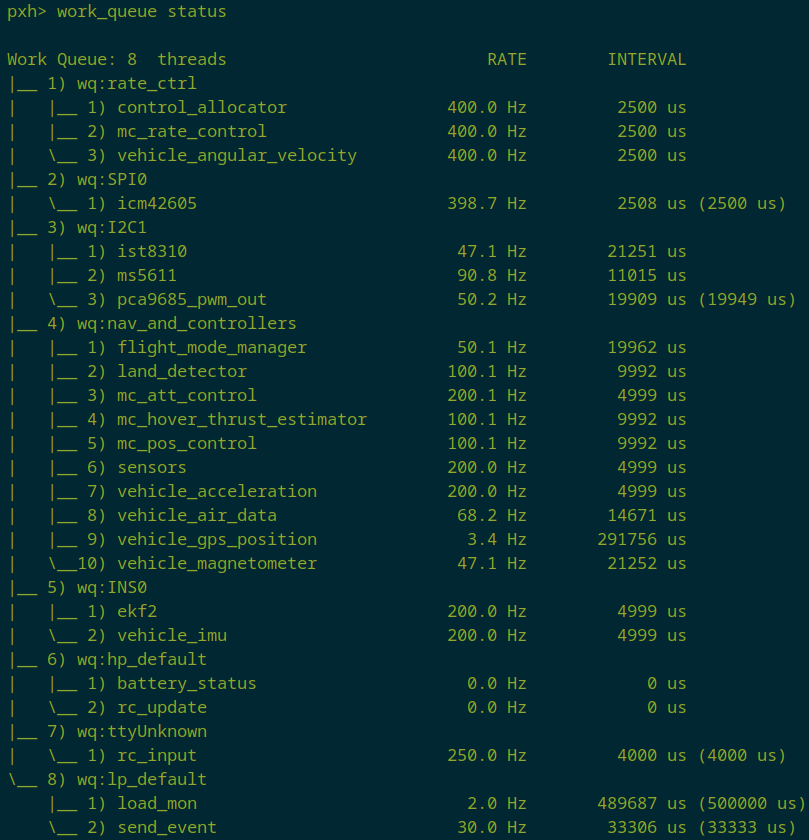
\includegraphics[width=0.5\textwidth]{./img/png/sspfs-px4-validation} 
%   \caption[SSPFS: PX4 system analysis]{SSPFS: PX4 system analysis via \lstinline{work_queue status}}%
%   \label{fig:sspfs-px4-validation}
% \end{figure}

% \begin{figure}
%   \centering
%   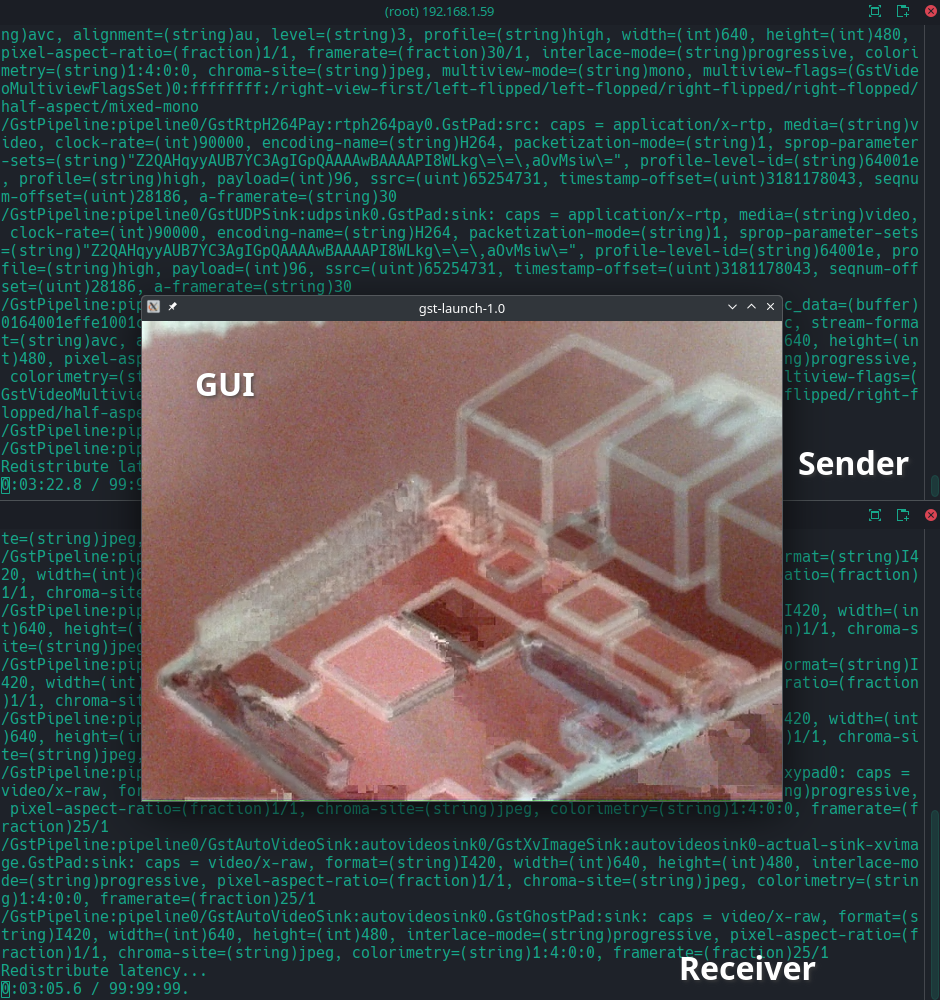
\includegraphics[width=0.5\textwidth]{./img/png/sspfs-cam-qgc} 
%   \caption{SSPFS: Video surveillance application}%
%   \label{fig:sspfs-cam-qgc}
% \end{figure}

% Figure environment with subfigures
\begin{figure}[!hbt]
  \centering
  % Row 1: Two half-width images
  \begin{subfigure}[t]{0.49\textwidth}
    \centering
    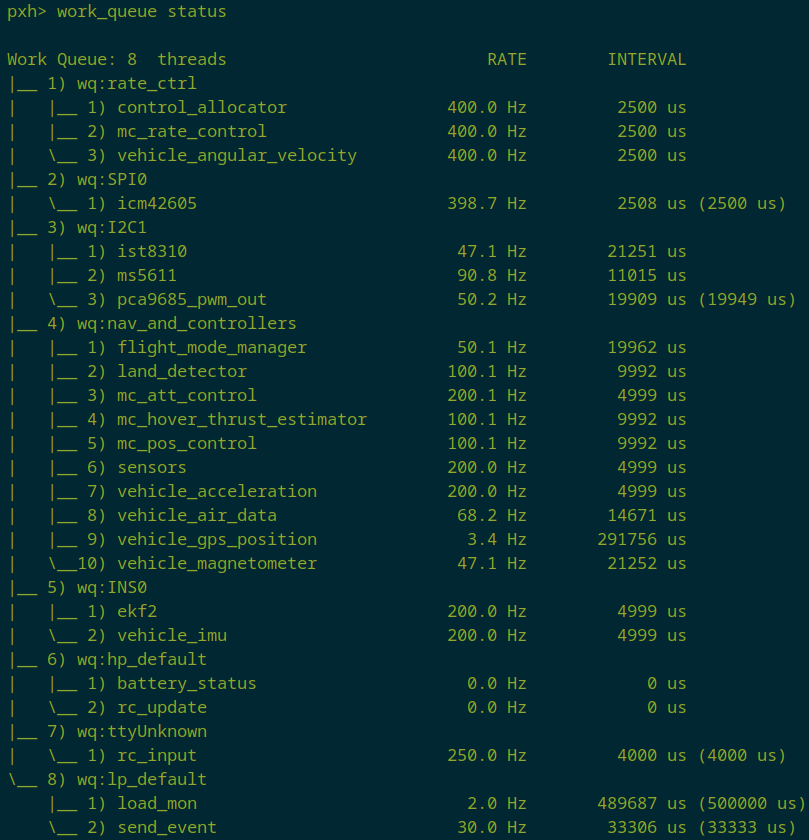
\includegraphics[width=1.0\textwidth]{./img/png/sspfs-px4-validation} 
    \caption{PX4}%
    \label{fig:sspfs-app-validation-1}
  \end{subfigure}
%  \\[0.5\baselineskip] % Vertical space after first row
  \begin{subfigure}[t]{0.49\textwidth}
    \centering
    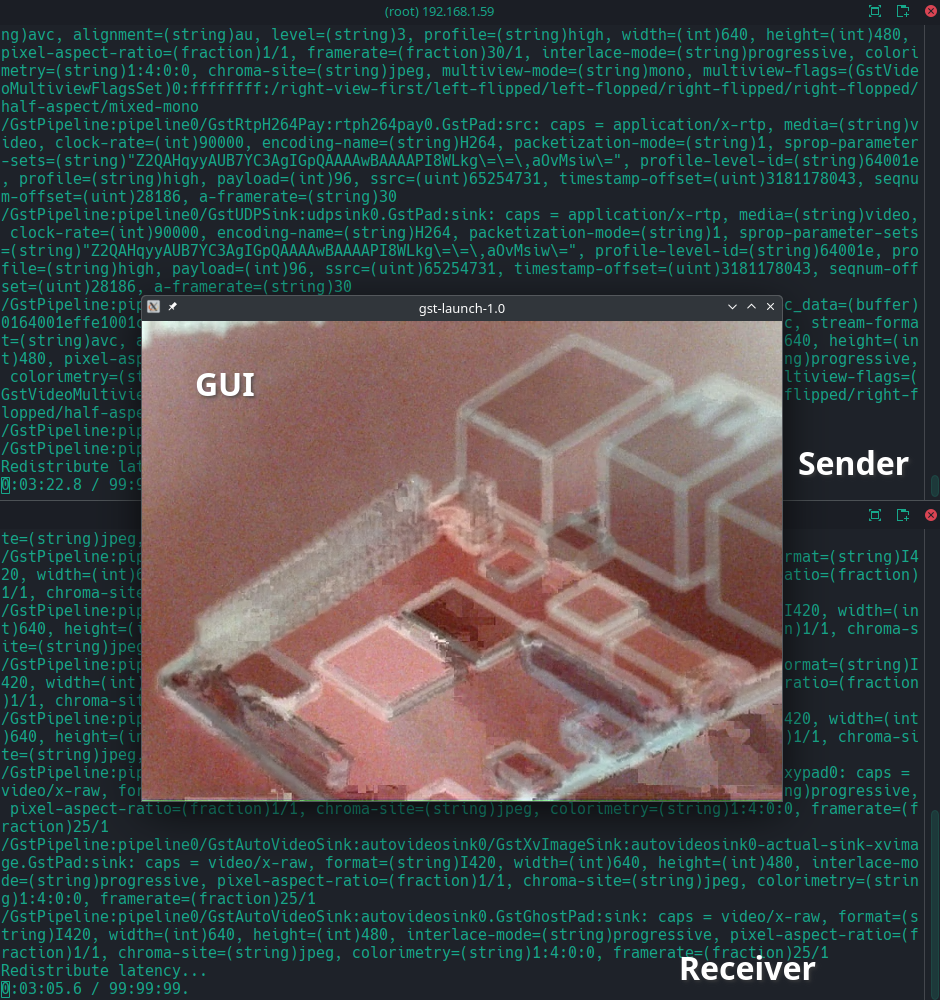
\includegraphics[width=\linewidth]{./img/png/sspfs-cam-qgc} % Use \linewidth inside subfigure
    \caption{Video surveillance}%
    \label{fig:sspfs-app-validation-2}
  \end{subfigure}
  \caption{SSPFS: validation of application software}
  \label{fig:sspfs-app-validation}
\end{figure}



\section{Functional tests}
\label{sec:functional-tests}
Fig.~\ref{fig:uav-main-eval-kmod} outlines the functional test methodology,
which evaluates system resilience when compromised by malicious actors. Attack
scenarios were emulated through the deployment of malicious components, either
in user space (\lstinline{crash_app}) or kernel space
(\lstinline{crash_mod.ko}), to the \gls{uspfs} and \gls{sspfs}.
In the unsupervised configuration, malicious components execute directly on the
host Linux \gls{os}, and thus we expect a system-wide crash. This causes both
non-critical (video surveillance) and critical (PX4) stacks to terminate
abruptly, leading to a catastrophic \gls{uav} failure. On the other hand, in the
\gls{sspfs}, we deploy malicious components exclusively to the Companion
\gls{vm}, emulating a compromise in the non-critical system, possibly exploited
through the Wi-Fi communication. In this case, we expect a hypervisor fault
to be triggered, causing a crash in the Companion \gls{vm}. Consequently, the
non-critical stack terminates while the critical PX4 stack remains operational,
maintaining flight capability.
%
This comparative analysis demonstrates the supervised architecture's ability to
contain faults within non-critical domains, preserving essential flight
functions during security compromises.

\begin{figure}[!hbt]
  \centering
  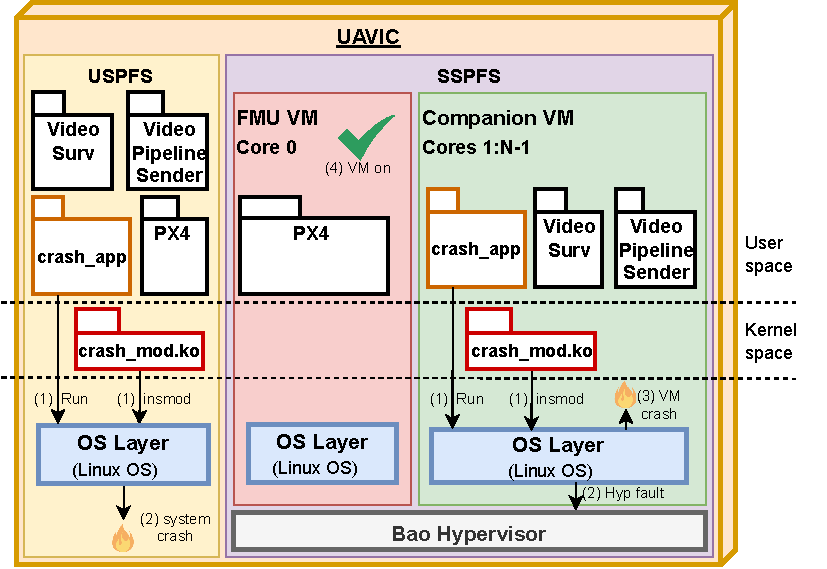
\includegraphics[width=0.8\textwidth]{./img/pdf/uav-main-eval-funcTest} 
%  \includesvg[width=1.0\textwidth]{./img/virtualization.svg} 
  %\caption[Virtualization mind map]{Virtualization mind map}%
  \caption{Functional tests' overview}%
  \label{fig:uav-main-eval-kmod}
\end{figure}

\subsection{Privileged mode}
\label{sec:privileged-mode}
Malicious actors gaining privileged system access, either by gaining superuser
privileges or through corrupted kernel modules, pose significant threats. This
section examines system vulnerability to privileged-mode attacks through
malicious kernel module deployment.

% \subsubsection{Kernel Panic Attack}
% \label{sec:panic}
A fundamental kernel attack vector involves explicit \lstinline{panic}
invocation, signaling unrecoverable system states.
Listing~\ref{lst:kmod-panic} (line 5) implements this approach and shows the
basic kernel module structure. We will refer to other kernel modules
implementation in the online repository, available at \lstinline{eval/kmod/}~\cite{thesis-sw-github}.
When the kernel module is executed, we expect: (1) local interrupts and
preemption are disabled; (2) secondary cores are halted; (3) a
\lstinline{Forced kernel panic!} message is logged; (4) system reboots after a
timeout expiration, or remains freezed in a infinite loop.

\begin{longlisting}
\centering
\inputminted[]{c}{./listing/kmod_panic.c}
\caption[Functional tests: implementation of the panic kernel module]{Functional
  tests: implementation of the Panic kernel module (see
  \lstinline{panic_module.c}~\cite{thesis-sw-github})}
\label{lst:kmod-panic}
\end{longlisting}

Fig.~\ref{fig:kmod-panic-test-uspfs} demonstrates panic module testing in the
\gls{uspfs} system. We boot the system boot via UART (1). Then we open another
terminal and interact with the system via SSH over Wi-Fi to insert the malicious
kernel module (2). As the remote connection freezed, we tested the network
connection and verified that \gls{uspfs} was unreachable, (3) confirming a
catastrophic \gls{uav} failure.

% Figure environment with subfigures
\begin{figure}[!hbt]
  \centering
  % Row 1: Two half-width images
  \begin{subfigure}[t]{0.8\textwidth}
    \centering
    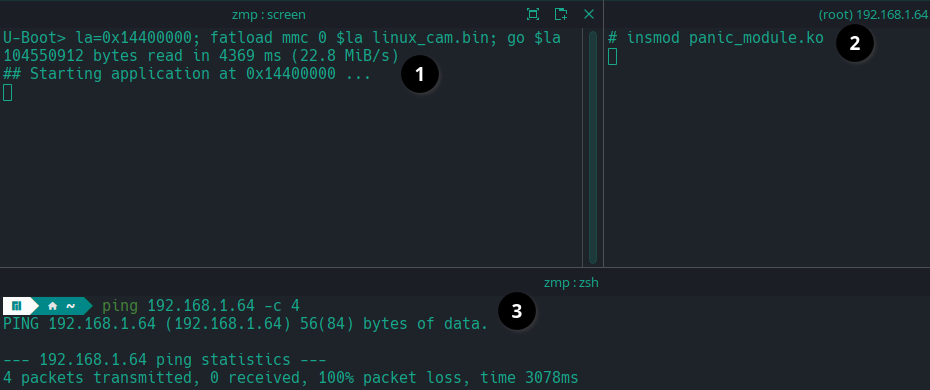
\includegraphics[width=1.0\textwidth]{./img/png/kmod-panic-test-annot} 
    \caption{USPFS}%
    \label{fig:kmod-panic-test-uspfs}
  \end{subfigure}
%  \\[0.5\baselineskip] % Vertical space after first row
  \begin{subfigure}[t]{0.8\textwidth}
    \centering
    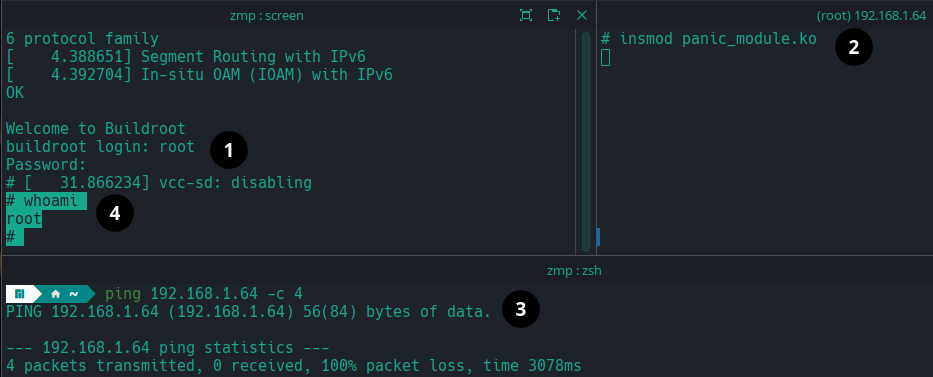
\includegraphics[width=\linewidth]{./img/png/kmod-panic-test-bao-annot} % Use \linewidth inside subfigure
    \caption{SSPFS}%
    \label{fig:kmod-panic-test-sspfs}
  \end{subfigure}
  \caption{Functional tests: panic kernel module testing}
  \label{fig:kmod-panic-test}
\end{figure}

% \begin{figure}[!hbt]
%   \centering
%   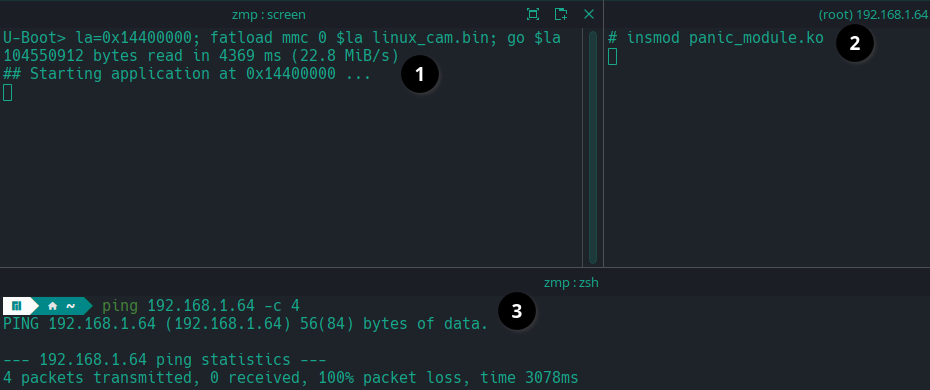
\includegraphics[width=0.8\textwidth]{./img/png/kmod-panic-test-annot} 
%   \caption{Functional tests: panic kernel module testing -- USPFS}%
%   \label{fig:kmod-panic-test}
% \end{figure}

We then performed an equivalent test in the \gls{sspfs} system (Fig.~\ref{fig:kmod-panic-test-sspfs}). We started the
system using U-boot's \gls{uart} boot console, which is the later used by Bao
and the PX4 \gls{vm}, enabling us to login into the system (1). Then, we connect
using \gls{ssh} over Wi-Fi to the Companion \gls{vm} and insert the malicious
kernel module (2). We immediately detected a freeze on that terminal, and thus,
we tested and verified the network connection was down, indicating a crash in
the Companion \gls{vm} (3). However, the PX4 \gls{vm} remained operational (4),
confirming \gls{uav} integrity.
%
These results demonstrate Bao hypervisor's capacity to consolidate
mixed-criticality stacks while maintaining domain isolation during
privileged-mode attacks.

% \begin{figure}[!hbt]
%   \centering
%   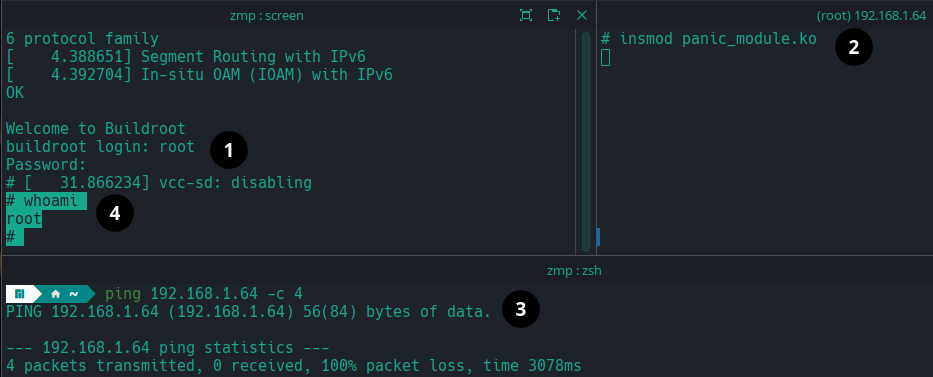
\includegraphics[width=0.8\textwidth]{./img/png/kmod-panic-test-bao-annot} 
%   \caption{Functional tests: panic kernel module testing -- SSPFS}%
%   \label{fig:kmod-panic-test-bao}
% \end{figure}

% \subsubsection{Memory corruption}
% \label{sec:mem-corrupt}
A memory corruption attack exploits writes to unmapped physical addresses to
compromise the system. The kernel module's source code is available in the
online repository (\lstinline{memcorrupt_module.c}~\cite{thesis-sw-github}).
The module maps a valid but non-existent physical address to kernel virtual
space (line 27) and writes data to this address (line 36), which we expect 
to cause a crash due to lack of physical backing~\cite{iomapLinux}.
We applied
the same testing procedure to the \gls{uspfs} and \gls{sspfs} systems, obtaining
consistent results, i.e., the \gls{sspfs}'s critical system survives while the
whole \gls{uspfs} system. Consequently, the \gls{uav} survives in the first
case, but suffers a catastrophic failure in the second one.

% Fig.~\ref{fig:kmod-memcorrupt-test} demonstrates memory corruption testing in the \gls{uspfs} system:
% \begin{itemize}[noitemsep,topsep=0pt]
% \item System boot via UART (top left, 1)
% \item Remote module insertion via SSH over Wi-Fi (top right, 2) using invalid address \lstinline{0x8_0000_0000} (beyond Raspberry Pi 4's \lstinline{0x7_FFFF_FFFF} range~\cite{rpi4-bcm2711})
% \item Resultant network unreachability (bottom, 3) confirming catastrophic UAV failure
% \end{itemize}

% \begin{figure}[!hbt]
%   \centering
%   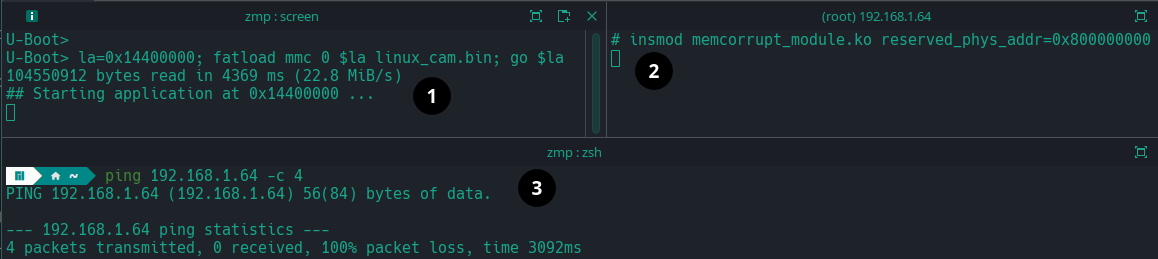
\includegraphics[width=1.0\textwidth]{./img/png/kmod-memcorrupt-test-annot} 
%   \caption{Functional tests: Memory corruption kernel module testing -- USPFS}%
%   \label{fig:kmod-memcorrupt-test}
% \end{figure}

% Fig.~\ref{fig:kmod-memcorrupt-test-bao} shows equivalent testing in the \gls{sspfs} system:
% \begin{itemize}[noitemsep,topsep=0pt]
% \item Shared UART boot console (Bao/PX4 VM, top left, 1)
% \item Malicious module insertion in Companion VM (SSH over Wi-Fi, top right, 2) using \lstinline{0x8_0000_0000}
% \item Hypervisor fault triggered at invalid virtual address (3)
% \item Companion VM network failure (bottom, 4)
% \item Maintained PX4 VM operation (5) preserving UAV functionality
% \end{itemize}

% \begin{figure}[!hbt]
%   \centering
%   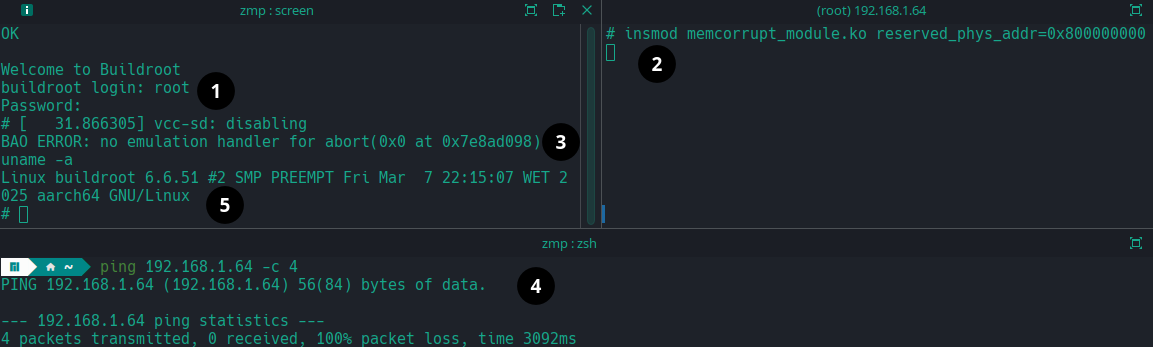
\includegraphics[width=1.0\textwidth]{./img/png/kmod-memcorrupt-test-bao-annot} 
%   \caption{Functional tests: testing of the memory corruption kernel module -- SSPFS}%
%   \label{fig:kmod-memcorrupt-test-bao}
% \end{figure}

% \subsubsection{Memory exhaustion}
% \label{sec:mem-exhaustion}
Memory exhaustion attacks represent another viable method to compromise the
system compromise by depleting the available memory.
The kernel module's source code is available in the
online repository (\lstinline{memhog_module.c}~\cite{thesis-sw-github}).
The attack methodology involves: (1) adjusting the \gls{oom} score of the
executing kernel thread to minimum priority (line 11) which effectively
reduces the likelihood of termination by the \gls{oom} killer during memory
pressure; (2) entering an infinite loop (line 15) that repeatedly allocates
single memory pages and locks pages (line 20) to prevent reclamation. This
permanently "hogs" memory resources, preventing reclamation even under severe
memory constraints.
%
We applied
the same testing procedure to the \gls{uspfs} and \gls{sspfs} systems, once
again with the same outcomes: the \gls{sspfs}'s critical system (and \gls{uav})
survives while the whole \gls{uspfs} system crashes.

% Fig.~\ref{fig:kmod-memhog-test} and Fig.~\ref{fig:kmod-memhog-test-bao} demonstrate memory exhaustion testing in the \gls{uspfs} and \gls{sspfs} systems respectively. Consistent with previous attack vectors, results show:
% \begin{itemize}[noitemsep,topsep=0pt]
% \item Catastrophic system failure in the unsupervised (\gls{uspfs}) configuration
% \item Contained failure limited to the Companion VM in the supervised (\gls{sspfs}) architecture
% \end{itemize}

% \begin{figure}[!hbt]
%   \centering
%   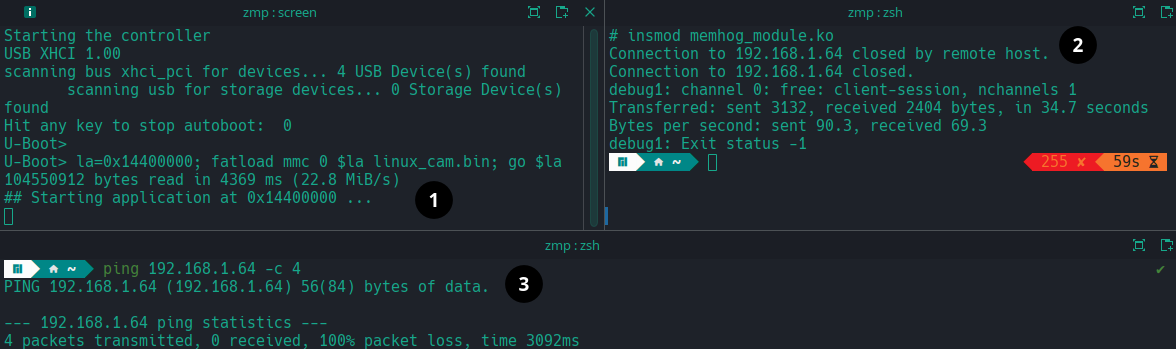
\includegraphics[width=1.0\textwidth]{./img/png/kmod-memhog-test-annot} 
%   \caption{Functional tests: testing of the memory exhaustion kernel module -- USPFS}%
%   \label{fig:kmod-memhog-test}
% \end{figure}

% \begin{figure}[!hbt]
%   \centering
%   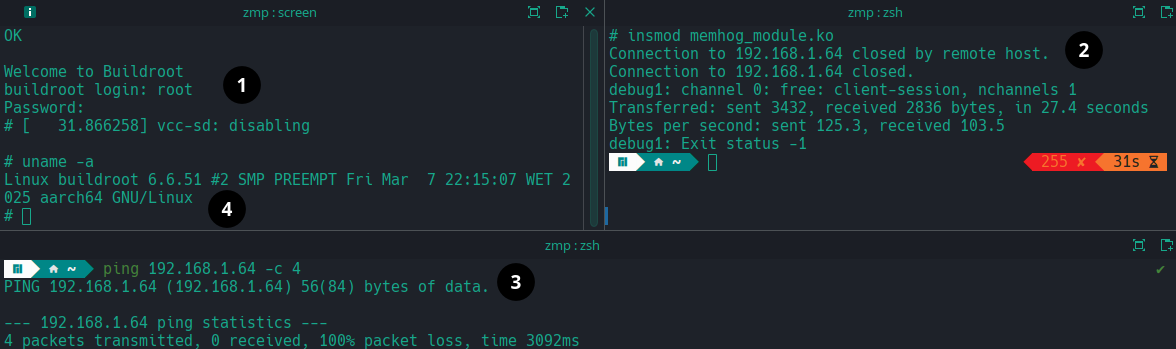
\includegraphics[width=1.0\textwidth]{./img/png/kmod-memhog-test-bao-annot} 
%   \caption{Functional tests: testing of the memory exhaustion kernel module -- SSPFS}%
%   \label{fig:kmod-memhog-test-bao}
% \end{figure}

% \subsubsection{Init process termination}
% \label{sec:kill-init-process}
Terminating the \lstinline{init} process provides a final attack vector for
system compromise.
The kernel module's source code is available in the
online repository (\lstinline{initkiller_module.c}~\cite{thesis-sw-github})
The process involves:
(1) acquiring a reference to the \lstinline{init} process (line 16);
(2) retrieving its memory layout (line 19);
(3) Iterating through all \glspl{vma} (line 28)
(4) and pin each page to prevent swapping (line 36) and corrupt its memory map
(line 42). This exhaustive corruption of the \lstinline{init} process's memory
space induces system failure.
We applied
the same testing procedure to the \gls{uspfs} and \gls{sspfs} systems, and
without surprise we assisted to the \gls{sspfs}'s critical system (and \gls{uav})
survival while the whole \gls{uspfs} system crashed.

% Fig.~\ref{fig:kmod-initkiller-test} and Fig.~\ref{fig:kmod-initkiller-test-bao} demonstrate init process termination testing in the \gls{uspfs} and \gls{sspfs} systems respectively. Results align with previous attack patterns:
% \begin{itemize}[noitemsep,topsep=0pt]
% \item Catastrophic failure in the unsupervised (\gls{uspfs}) configuration
% \item Contained failure limited to the Companion VM in the supervised (\gls{sspfs}) architecture
% \end{itemize}

% \begin{figure}[!hbt]
%   \centering
%   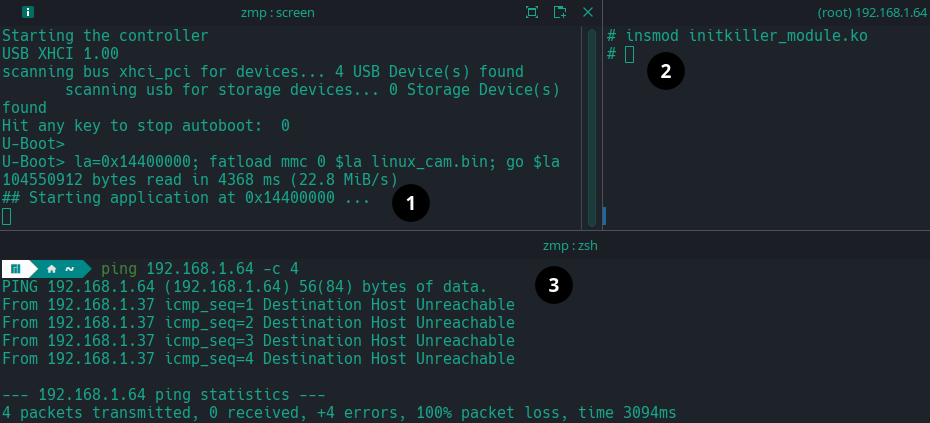
\includegraphics[width=1.0\textwidth]{./img/png/kmod-initkiller-test-annot} 
%   \caption{Functional tests: testing of the kill init process kernel module -- USPFS}%
%   \label{fig:kmod-initkiller-test}
% \end{figure}

% \begin{figure}[!hbt]
%   \centering
%   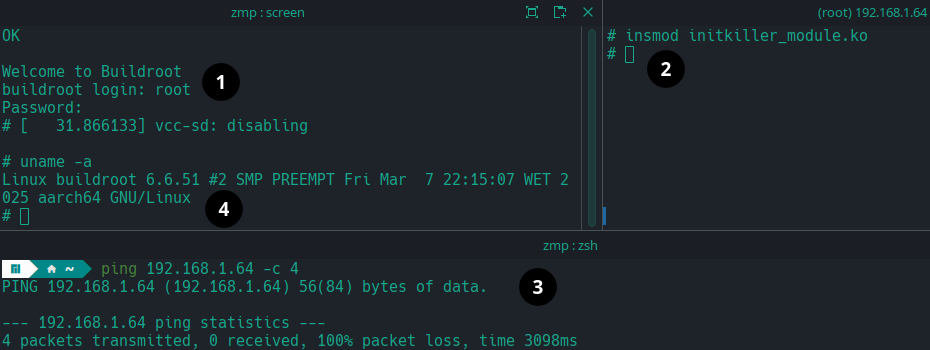
\includegraphics[width=1.0\textwidth]{./img/png/kmod-initkiller-test-bao-annot} 
%   \caption{Functional tests: testing of the kill init process kernel module -- SSPFS}%
%   \label{fig:kmod-initkiller-test-bao}
% \end{figure}

\subsection{Unprivileged mode}
\label{sec:unprivileged-mode}
User-space attacks present a reduced attack surface due to limited access to
critical resources. Thus, one common approach is to induce severe system
contention, which, while not causing literal crashes, significantly degrades performance,
potentially leading to a catastrophic failure due to the unresponsiveness of the
critical system.
The source code for the user space memory exhaustion application is available in the
online repository
(\lstinline{eval/userspace/memhog_module.c}~\cite{thesis-sw-github}). We
implemented this employing three parallel attack vectors:
(1) memory exhaustion
through infinite allocation while evading the \gls{oom} killer
(\lstinline{memory_attack()});
(2) process exhaustion via a "fork bomb" generating processes that modify shared
memory regions before hanging (\lstinline{process_attack()});
(3) and \gls{cpu} and \gls{io} starvation (\lstinline{cpu_io_attack()}) achieved
by reassigning the highest scheduling priority to this process (line 132), and
performing continuous random page reads (line 140), and forcing CPU rescheduling
(line 143).

A monitoring thread (\lstinline{status_thread()}) tracks: (1) elapsed execution
time; (2) free memory (\lstinline{sysinfo()});
(3) process count (\lstinline{sysinfo.procs});
(4) \gls{cpu} usage (\lstinline{/proc/stat})
(5) and \gls{cpu} load average (\lstinline{sysinfo.loads}).
The \lstinline{main()} function coordinates the attack: (1) recording start
time; (2) removing resource limits; (2) launching the monitoring thread; (4) (4)
initiating a child process for each attack; (5) and remaining online via a
non-optimizable infinite loop.

Fig.~\ref{fig:user-memhog-test-uspfs} demonstrates resource exhaustion testing in the
\gls{uspfs} system. We booted the system via UART (1) and connected to it via
\gls{ssh} over Wi-Fi (2). We then observed the system started to become unresponsive
(3), evidenced by \lstinline{ls} failure (3), with the system resources being
permanently allocated to the application (4). We can also observe that the
system remains online in the network, but is incapable of handling
requests. Thus, although the system continues to operate, it fails to service
any other application, such as PX4 or video surveillance, causing severe impact
on the flight performance of the \gls{uav}.

We then applied the same testing procedure to the \gls{sspfs} system
(Fig.~\ref{fig:user-memhog-test-sspfs}). We booted the system via UART, starting
the PX4 and Companion \glspl{vm}. After login into the PX4 \gls{vm} (1) we  
connected to the Companion \gls{vm} via \gls{ssh} over Wi-Fi (2). Then, we
started the memory exhaustion application in the Companion \gls{vm}, and after
some time, we observed this subsystem was unresponsive (3), dedicating the
system resources to the running application (4). However, in this case, we
observed that we can interact normally with the PX4 \gls{vm}, i.e., only the
non-critical system was affected, and consequently, the \gls{uav} remains operational.
%
These results confirm the Bao hypervisor's capacity to maintain critical flight
functions even under severe non-critical system contention, demonstrating
effective consolidation with domain isolation.

\begin{figure}[!hbt]
  \centering
  % Row 1: Two half-width images
  \begin{subfigure}[t]{0.7\textwidth}
    \centering
    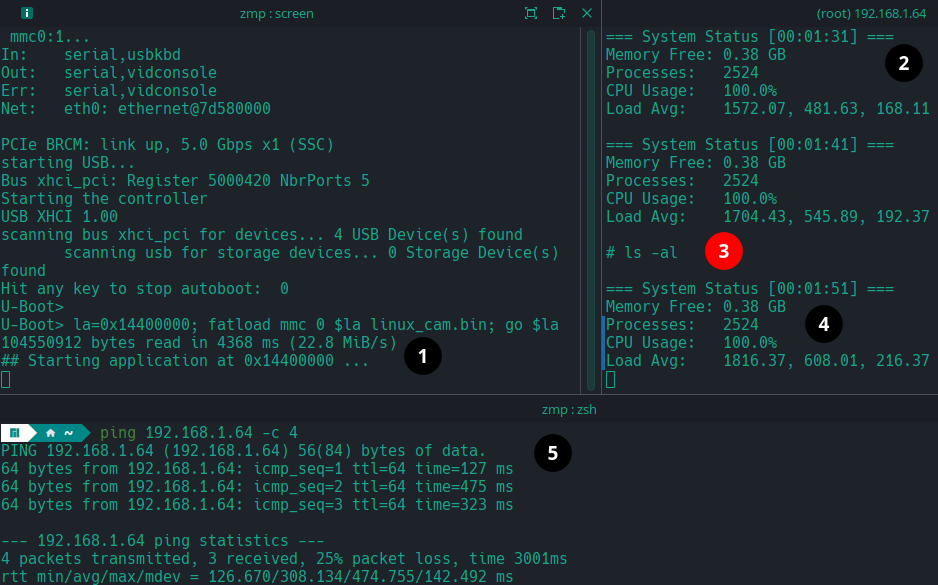
\includegraphics[width=1.0\textwidth]{./img/png/user-memhog-test-annot} 
    \caption{USPFS}%
    \label{fig:user-memhog-test-uspfs}
  \end{subfigure}
%  \\[0.5\baselineskip] % Vertical space after first row
  \begin{subfigure}[t]{0.7\textwidth}
    \centering
    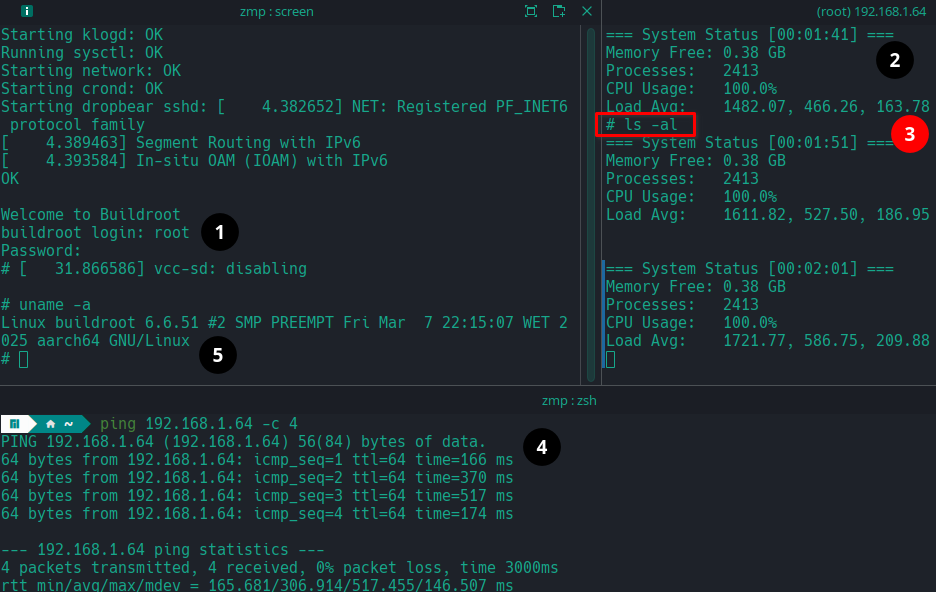
\includegraphics[width=\linewidth]{./img/png/user-memhog-test-bao-annot} % Use \linewidth inside subfigure
    \caption{SSPFS}%
    \label{fig:user-memhog-test-sspfs}
  \end{subfigure}
  \caption{Functional tests: user space resource exhaustion application}
  \label{fig:user-memhog-test}
\end{figure}


% \begin{figure}[!hbt]
%   \centering
%   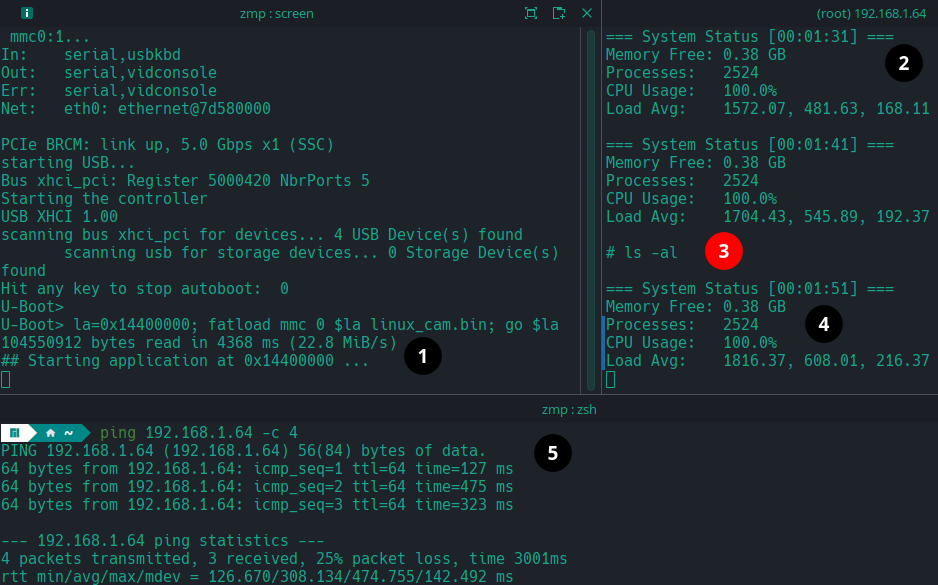
\includegraphics[width=1.0\textwidth]{./img/png/user-memhog-test-annot} 
%   \caption{Functional tests: Resource exhaustion application testing -- USPFS}%
%   \label{fig:user-memhog-test}
% \end{figure}

% \begin{figure}[!hbt]
%   \centering
%   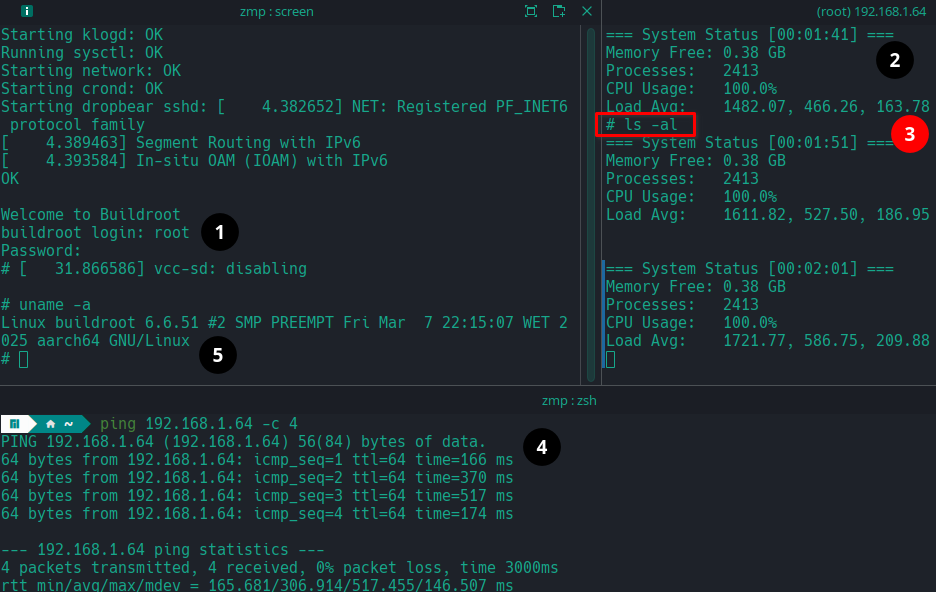
\includegraphics[width=1.0\textwidth]{./img/png/user-memhog-test-bao-annot} 
%   \caption{Functional tests: Resource exhaustion application testing -- SSPFS}%
%   \label{fig:user-memhog-test-bao}
% \end{figure}

\section{Bao benchmarks}
\label{sec:bao-benchmarks}
Previous research extensively benchmarked the Bao hypervisor against relevant
competitors in \gls{mcs} contexts~\cite{martins2023shedding,costaIRQColoring2023}.
We adopted the same methodology while focusing exclusively on performance metrics.
We started by establishing the baseline performance of the \gls{uspfs} system
(native execution) and quantifying performance degradation in the \gls{sspfs}
system after adding the Bao hypervisor. Performance degradation (PD) is
given by Equation~\ref{eq:perform-deg} as the relative overhead in execution
time (ET):

\begin{equation}
  \label{eq:perform-deg}
  PD (\%) =
\frac{ET_{\text{SSPFS}} - ET_{\text{USPFS}}}{ET_{\text{USPFS}}} \cdot 100
\end{equation}

% \[
% \text{Degradation} =
% \frac{\text{Execution\_time}_{\text{SSPFS}}}{\text{Execution
%     \_time}_{\text{USPFS}}} \cdot 100
% \]

The testing framework utilizes the MiBench Embedded Benchmarks'
\gls{aics}~\cite{guthaus2001mibench}, especially suited for industrial and
automotive embedded systems. It features two variants: a small-scale
variant with minimized input dataset replicating resource-constrained
environments, and a large-scale variant with expanded dataset approximating
real-world operational loads. We use \lstinline{perf}~\cite{perfLinux} to
accurately measure the execution time and track the microarchitectural events in
the Linux \glspl{vm}, while baremetal guests use the Arm Generic timer (10 ns
resolution) with a custom \gls{pmu} driver. The monitored events are registered
at their respective exception levels, including: (1) instruction count; (2)
\gls{tlb} accesses/refills; (3) cache accesses/refills; (4) exceptions; (5) and interrupts.
%
We analyze interference between guests by deploying a custom baremetal guest
with three \glspl{vcpu} performing continuous write operations to a buffer with
the \gls{llc} size. This represents a significant workload, although, not
necessarily, the worst-case scenario.

Fig.~\ref{fig:uav-main-eval-mibench} outlines the benchmarking workflow
comprising three stages: compiling guests, testing the performance, and logging
the results. We start by building the Linux guest (MiBench suite +
\lstinline{perf}) and interference guest using SheddingLight repository
instructions~\cite{shedlightRepo}.
To test the performance we evaluate the
baseline \gls{uspfs} and four \gls{sspfs} configurations: \lstinline{mibench}
(Linux guest + Bao), \lstinline{mibench+col} (+ cache coloring),
\lstinline{mibench+interf} (+ interference guest), and
\lstinline{mibench+interf+col} (+ interference \& coloring).
%
The Experiment workflow details the generic evaluation process. We start by
deploying an executable \lstinline{BIN} (\lstinline{linux.bin} or
\lstinline{bao.bin}) to the \gls{sd} card (1). Then, we set up a persistent
connection (green background) between \gls{gcs} and \gls{uavic} to capture the
logs (2). We power on the \gls{uavic} platform (3) and after U-Boot
initializes (4), we start the primary binary \lstinline{BIN} which dumps the
results to a log file (8). There are cases where we need to execute a second
second binary \lstinline{BIN2}, for example, when running the whole MiBench
suite, redirecting the results to one common file (7). We then close the file
and plot the results using a Python script. All MiBench related files are stored
in the online repository (see \lstinline{mibench/}~\cite{thesis-sw-github}),
namely the configurations used, the log files, and the plotting scripts.

\begin{figure}[!hbt]
  \centering
  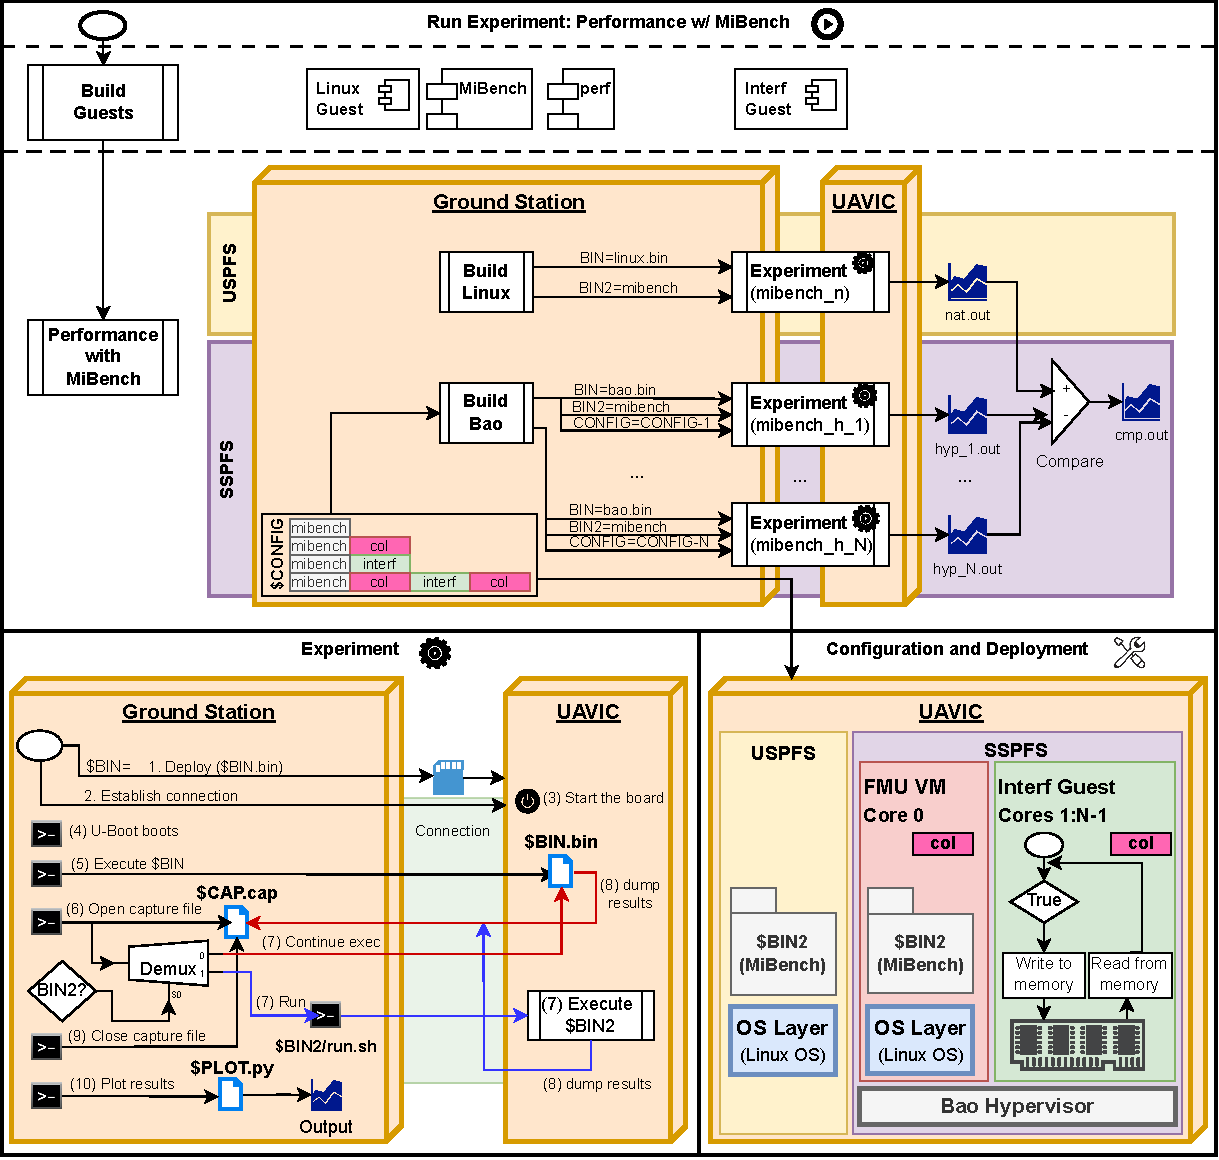
\includegraphics[width=1.0\textwidth]{./img/pdf/uav-main-eval-mibench} 
  \caption{Bao performance benchmarking workflow}%
  \label{fig:uav-main-eval-mibench}
\end{figure}

Fig.~\ref{fig:plot-performDeg-Base} shows the relative performance degradation
for the MiBench \gls{aics} across three configurations:
(1) \hlighthex{0097FF}{000000}{\textbf{baremetal-noMail}} -- native
execution without mailbox driver patch;
(2)
\hlighthex{399334}{000000}{\textbf{bao-noMail}} -- Linux OS + Bao without
mailbox driver patch.
(3)
\hlighthex{FF9E00}{000000}{\textbf{bao}} -- MiBench on Linux OS + Bao
hypervisor. The average native execution times are shown below each benchmark.
%
The performance degradation remains minimal, particularly for longer-running
benchmarks (\lstinline{large} suffix, e.g., \lstinline{basicmath large},
\lstinline{qsort large}). Furthermore, we can observe the mailbox driver patch
introduces negligible overhead, while the Bao hypervisor's contribution to performance degradation is small.

\begin{figure}[!hbt]
  \centering
  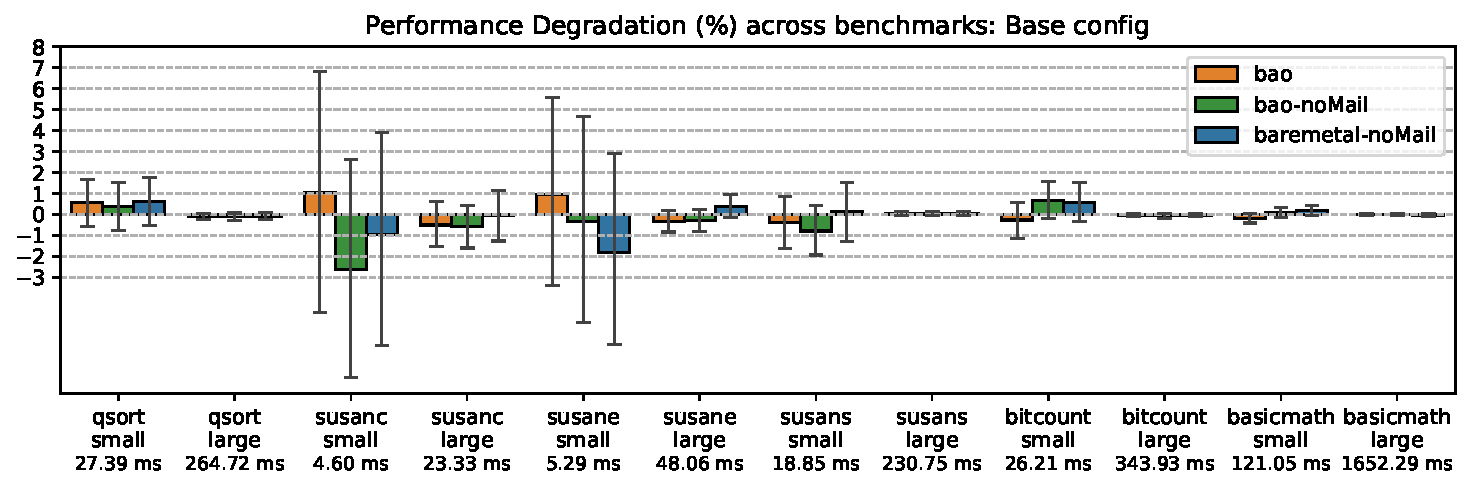
\includegraphics[width=1.0\textwidth]{./img/pdf/plot-performDeg-Base} 
  \caption{Relative performance degradation (\%) for MiBench AICS}%
  \label{fig:plot-performDeg-Base}
\end{figure}


Fig.~\ref{fig:plot-performDeg-Interf} presents relative performance degradation
for the MiBench \gls{aics} under cache partitioning and interference across
three configurations: (1) \hlighthex{FF9E00}{000000}{\textbf{bao+col}} --
MiBench on VM1 with 2 cache colors; (2)
\hlighthex{399334}{000000}{\textbf{bao+interf}}: MiBench on VM1 with
interference guest on VM2 using 3 CPUs; (3) and
\hlighthex{0097FF}{000000}{\textbf{bao+interf+col}} -- MiBench on VM1 with 2
colors + interference guest on VM2 using 3 CPUs and 2 colors. Cache colors were
evenly distributed across virtual machines, with average native execution times
provided below each benchmark.
%
We observe significant performance degradation under interference
conditions, particularly affecting short-duration benchmarks (\lstinline{small}
suffix, e.g., \lstinline{susanc small}, \lstinline{susane small}). This
degradation is attenuated in longer-running benchmarks, while cache partitioning
via page coloring consistently mitigates the performance impacts for VM1.

\begin{figure}[!hbt]
  \centering
  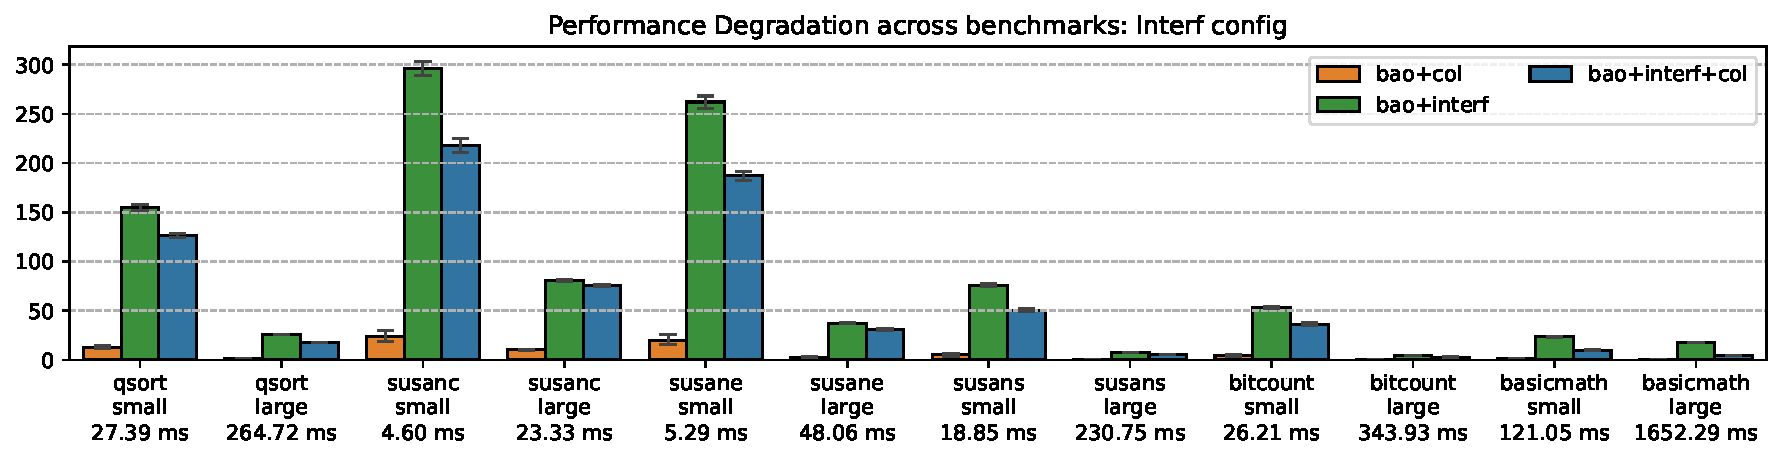
\includegraphics[width=1.0\textwidth]{./img/pdf/plot-performDeg-Interf} 
  \caption{Relative performance degradation (\%) for MiBench AICS under cache partitioning and interference}%
  \label{fig:plot-performDeg-Interf}
\end{figure}

% Finally, Fig.~\ref{fig:uav-main-eval-interf} illustrates the configuration and
% deployment of the benchmarking workflow on the \gls{uavic} platform. In the
% \gls{uspfs} system, we run MiBench on top of \gls{uspfs} Linux \gls{os}. Then,
% in the \gls{sspfs} system we have two variants: single-guest or dual-guest. In
% the single-guest -- \gls{fmu} \gls{vm} -- the MiBench suite runs on top of the
% Linux \gls{os} which runs on top of the Bao hypervisor. The pollution of caches
% and \glspl{tlb} by the hypervisor may affect guest performance, and thus, cache
% coloring is analyzed to mitigate this effect. In the dual-guest --- \gls{fmu} +
% Interference --- an interference guest is added to generate contention in the
% system, by continuously writing to memory 

% \begin{figure}[!hbt]
%   \centering
%   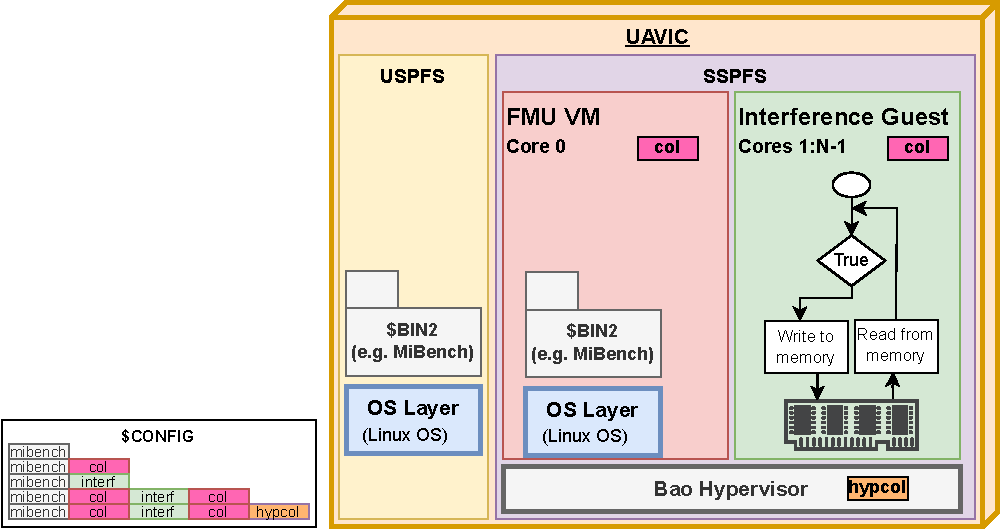
\includegraphics[width=1.0\textwidth]{./img/pdf/uav-main-eval-interf} 
% %  \includesvg[width=1.0\textwidth]{./img/virtualization.svg} 
%   %\caption[Virtualization mind map]{Virtualization mind map}%
%   \caption{Bao's performance benchmarking workflow: configuration and deployment}%
%   \label{fig:uav-main-eval-interf}
% \end{figure}

\subsection{Guests benchmarking}
\label{sec:guests-benchmarking}
In this section we benchmark each \gls{vm} separately, using
application-specific metrics. Then, we use these metrics to compare the
\gls{uspfs} and \gls{sspfs} systems.

\subsubsection{FMU VM}
\label{sec:fmu-vm}
The \gls{fmu} \gls{vm} runs the PX4 flight stack atop a Linux OS managed by the
Bao hypervisor. We adapted the previous benchmarking methodology to profile the
PX4 application using \lstinline{perf}. Unlike the MiBench benchmarks, which
have a finite duration, the PX4 application runs continuously. This means we
must be able to stop the application and restart it. Fortunately, we can pass the \lstinline{--timeout} argument to \lstinline{perf}, which
forks to run PX4 until the timeout expires, while collecting performance data.
%
Listing~\ref{lst:perf-px4} shows the PX4 benchmarking procedure. We defined a
testing set of 5 warm-up runs and 20 test runs of 30-second duration each.
The \lstinline{px4_bench()} routine invokes \lstinline{perf} to profile the
application and provide the statistics for the predefined repetitions, events,
and timeout, executing the custom command to launch PX4.
We then define the events to track (line 18) and invoke \lstinline{px4_bench} to
conduct the warm-up and normal runs.

\begin{longlisting}
\centering
\inputminted[]{bash}{./listing/perfPX4.sh}
\caption{PX4 benchmarking using perf}
\label{lst:perf-px4}
\end{longlisting}

Execution time proved unsuitable for degradation measurement due to the forced
termination. Native execution averaged $30.044213 \pm 0.000613$ seconds, while
Bao execution averaged $30.04608 \pm 0.00199$ seconds, yielding a maximum
degradation of just 0.015\%. Instead, performance degradation was calculated
based on the instruction count (\lstinline{r08:uk} event). Native execution
recorded 3,077,590,067 events compared to Bao's 3,016,875,258 events, indicating
a small degradation of 1.97\%.

Nonetheless, for critical embedded systems like the \gls{fmu}, deadline compliance is
paramount. PX4 supports two task models: traditional tasks with separate
stacks/priorities, and resource-efficient work queue tasks that share
stacks/priorities. The latter is the preferred approach for optimized resource
utilization~\cite{px4WorkQueue}. Thus, we proceeded to profile the PX4
application, analyzing the task rate update in the work queues. We selected six critical flight operations~\cite{px4ModulesRefCtrl,px4ModulesRefDriver,px4ModulesRefSystem}:
(1) \lstinline{control_allocator}: takes torque and thrust setpoints as inputs
and outputs actuator setpoints;
(2) \lstinline{mc_rate_control}: for multicopter rate management; 
(3) \lstinline{pca9685_pwm_out}: handles \gls{pwm}-driven \gls{esc} motors via \gls{i2c};
(4) \lstinline{flight_mode_manager}: generates setpoints for all flight mode controllers; 
(5) \lstinline{mc_pos_control} implements position/velocity control; and 
(6) \lstinline{sensors} for data acquisition and publishing.

However, the implementation of this methodology is not straightforward. Firstly,
we need a way to interact with the application while it is running, so we can
query the work queue status. One simple method is using a shared \gls{fifo} file
to inject the required command into PX4. The \lstinline{px4_wq_run.sh} script
(see~\cite{thesis-sw-github}) implements this concept. The \lstinline{wq_run()}
function creates the shared \gls{fifo} (line 12), and starts PX4, immediately
capturing its process ID (lines 13-15). Then, we open the \gls{fifo}
for writing (line 24), and for each query we run the
\lstinline{work_queue status} command and sleep for 10 seconds (lines 28--32). After this, we
shutdown the application and perform some cleanup. We then invoke
\lstinline{perf} to perform 5 warm-up runs, followed by followed by 20 test runs
using the \lstinline{wq_run} function. Each test run collected
\lstinline{work_queue} metrics at 10-second intervals over a 3-minute duration,
totaling 18 queries per run. This process was executed on both native and Bao
hypervisor configurations for comparison.

Fig.~\ref{fig:px4-sched-overhead} shows the results of the experiments. In the
x-axis are indicated the work queue tasks and the mean update interval for the
native execution in microseconds (baseline). The bar plots indicate the mean
scheduling overhead (\%) and standard deviation for the Bao case. The scheduling
overhead is defined as the relative average overhead between the Bao and native
executions, given by Equation~\ref{eq:1} and Equation~\ref{eq:2}:

\begin{equation}
  \label{eq:1}
\mu_{ov} (\%) = \frac{\mu_{bao} - \mu_{bm}}{\mu_{bm}} \cdot 100
\end{equation}

\begin{equation}
  \label{eq:2}
\sigma_{ov} (\%) = \sqrt{ \left(\frac{\sigma_{bao}}{\mu_{bao}}\right)^{2} +
  \left(\frac{\sigma_{bm}}{\mu_{bm}}\right)^{2} } \cdot 100
\end{equation}

\begin{figure}[!hbt]
  \centering
  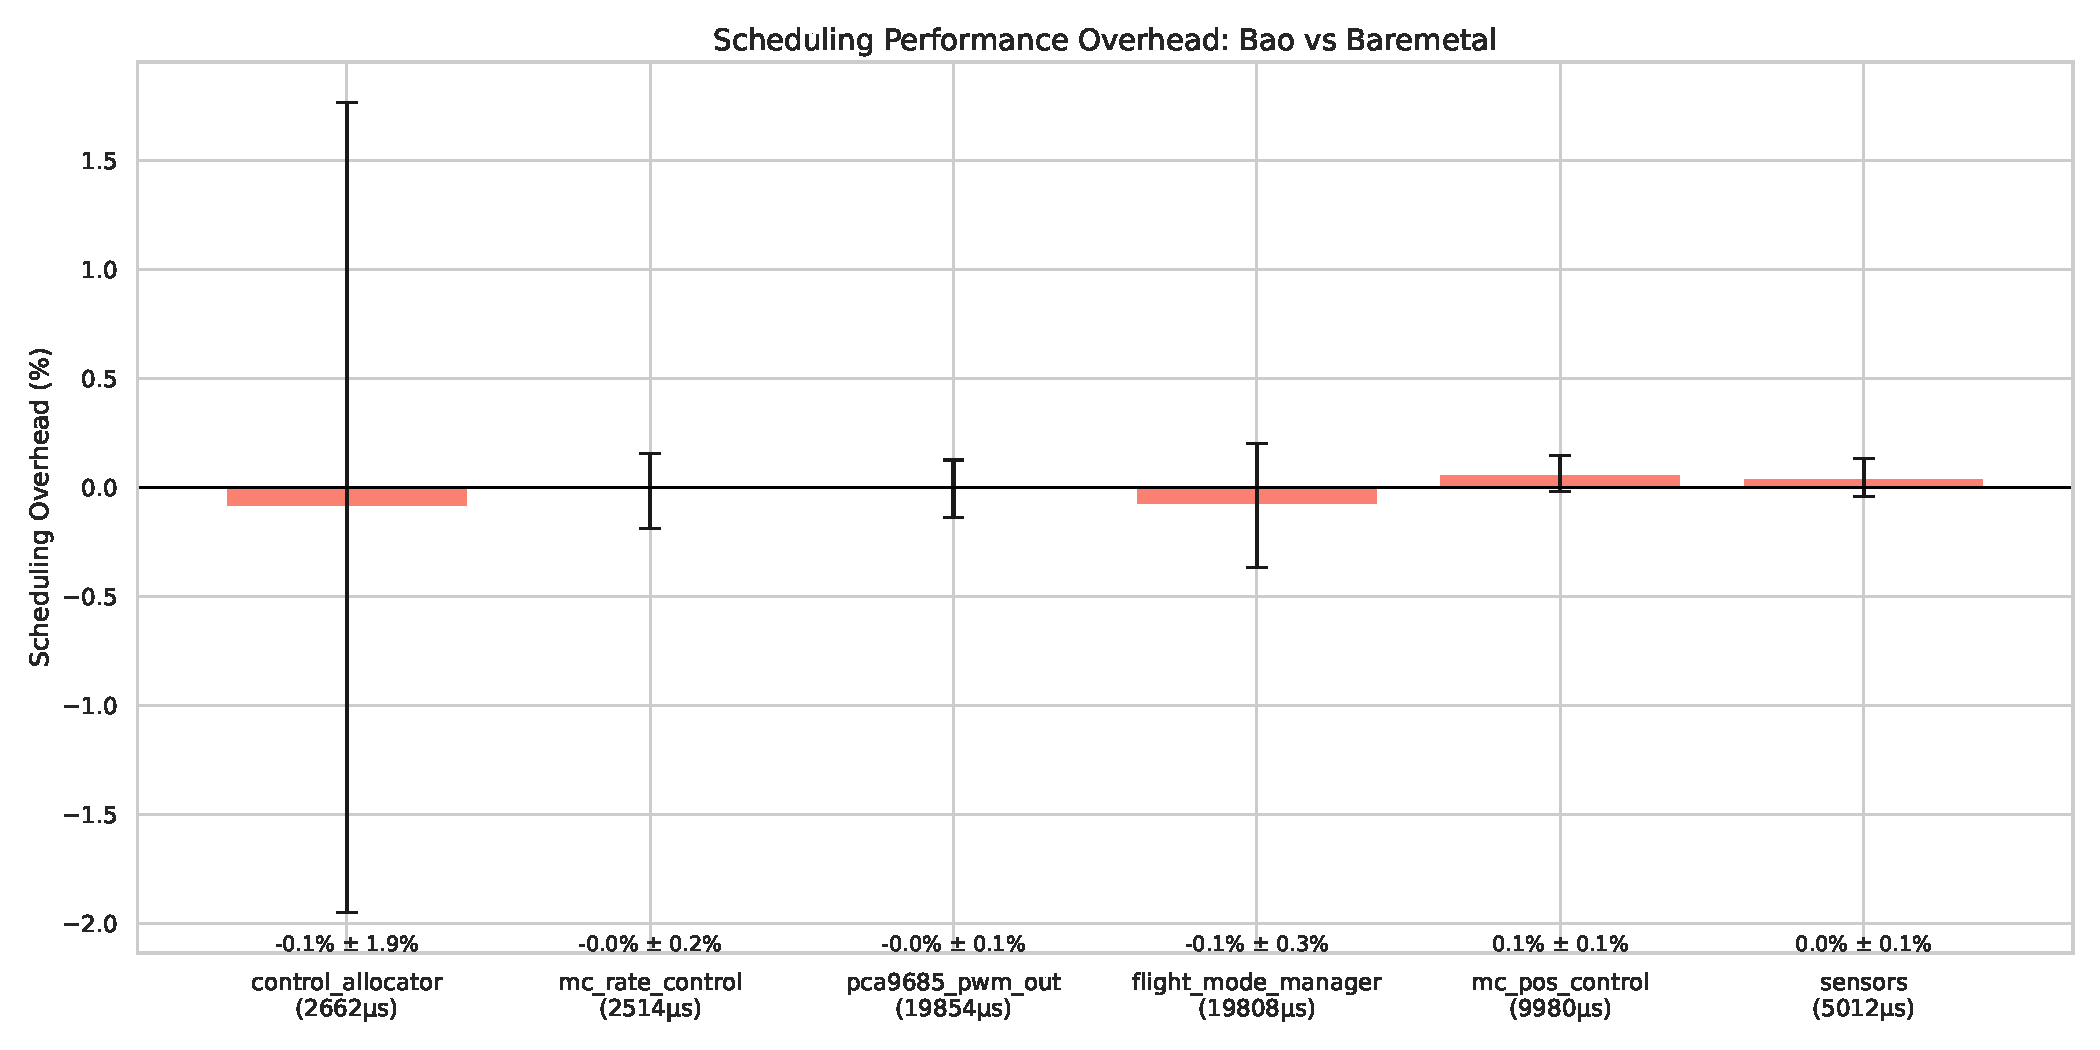
\includegraphics[width=1.0\textwidth]{./img/pdf/px4-sched-overhead} 
%  \includesvg[width=1.0\textwidth]{./img/virtualization.svg} 
  %\caption[Virtualization mind map]{Virtualization mind map}%
  \caption{PX4 tasks scheduling overhead}%
  \label{fig:px4-sched-overhead}
\end{figure}

The scheduling overhead is very low across work queue tasks. Most notably,
the \lstinline{pca9685_pwm_out} which is ultimately responsible for keeping the
\gls{uav} on the air, has a negligible scheduling overhead. On the other hand,
the \lstinline{control_allocator}, responsible for managing the control loop,
has a scheduling overhead of at most 2\%. These results demonstrate the
consolidation of the PX4 software stack into a single platform, enabled by the
Bao hypervisor, imposes minimum scheduling overhead in the critical system
(\gls{fmu}).

\subsubsection{Companion VM}
\label{sec:companion-vm}
The Companion \gls{vm} deploys the \lstinline{gstreamer} pipeline to manage
video surveillance and streaming to the \gls{gcs}. User experience constitutes a
critical factor in evaluating video surveillance service quality, with
particular emphasis placed on two key performance metrics: the sender's
\gls{fps} and frame latency (i.e. the delay between frame capture and
reception). However, system performance
may be significantly degraded by various external factors, particularly
fluctuations in \gls{gcs} \gls{cpu} utilization and network latency variations.

To objectively quantify the performance implications of platform consolidation,
we analyzed the frame rate at the \gls{uav} level. This approach isolates the
effects of system integration from external environmental variables. The
\lstinline{cam_fps.sh} (see~\cite{thesis-sw-github}) implements this method. We
conducted 5 warm-up runs and 20 test runs of the \lstinline{gstreamer} pipeline
for two minutes each, ater which we forcefully terminate it.
%
Fig.~\ref{fig:fps-cmp} presents the relative \gls{fps} performance degradation
between Bao and native execution across runs, calculated using Equation~\ref{eq:1} and Equation~\ref{eq:2}. Most runs show
degradation close to 0\% and top degradation is inferior to 2\%. The confidence
intervals are narrow, indicating precise measurements, and they include 0\%,
indicating that Bao introduces no statistically significant overhead to the
\gls{uav}'s camera frame rate.

\begin{figure}[!hbt]
  \centering
  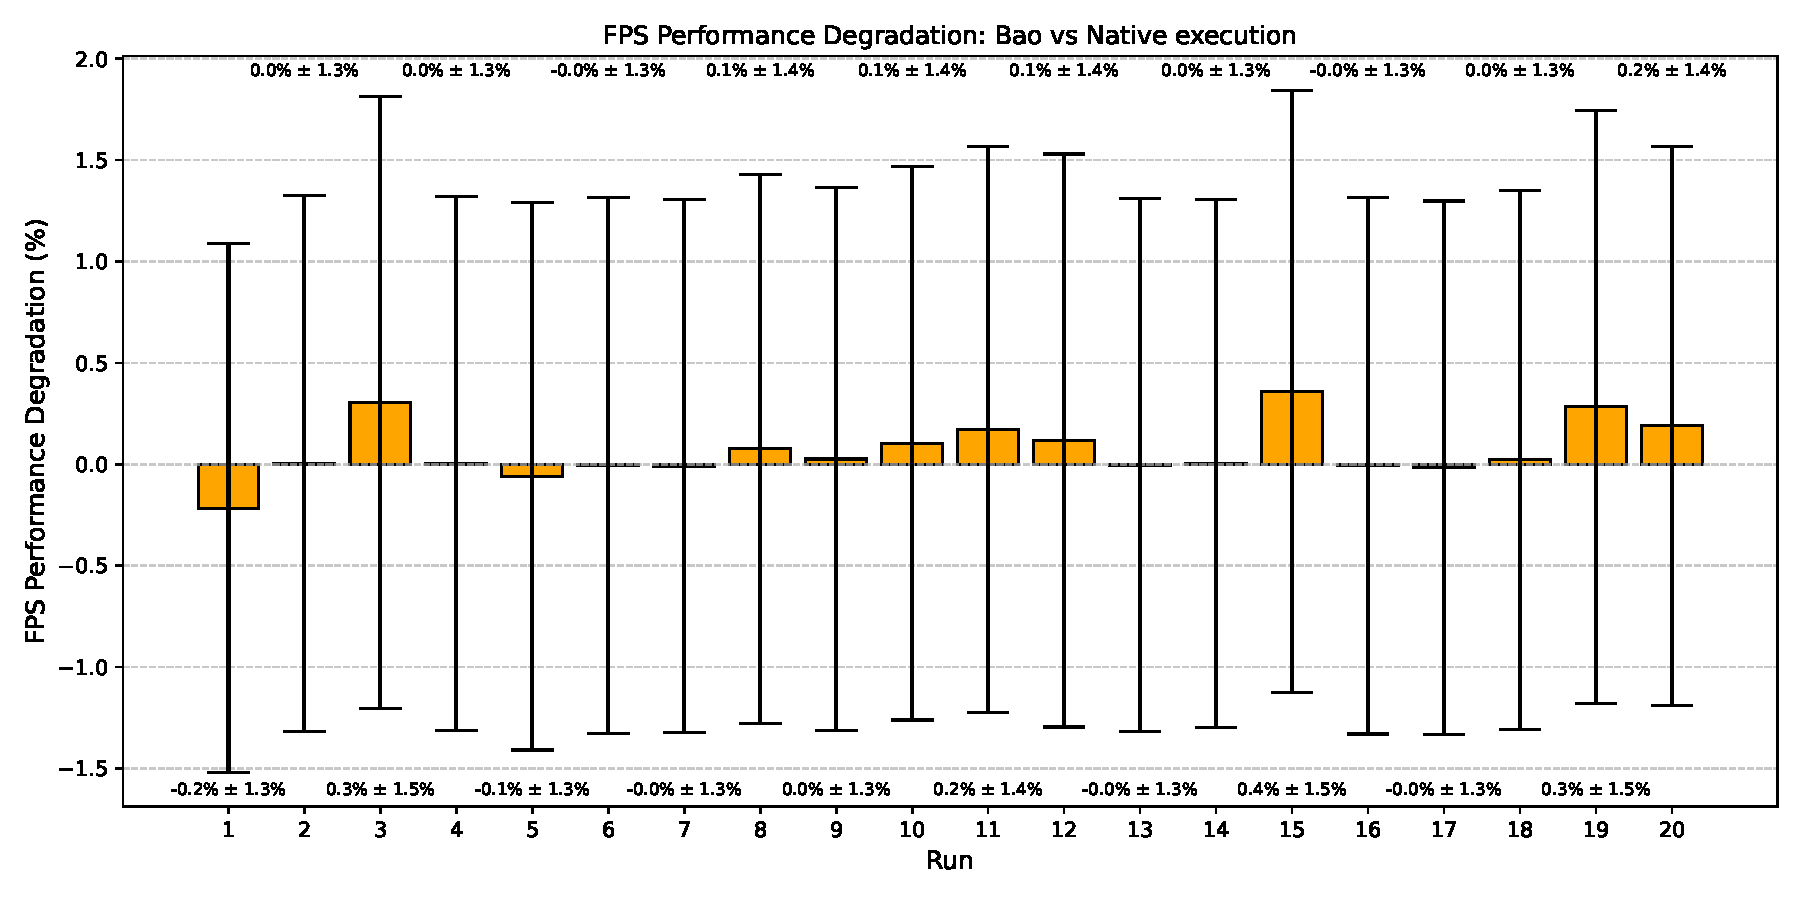
\includegraphics[width=1.0\textwidth]{./img/pdf/fps-cmp} 
%  \includesvg[width=1.0\textwidth]{./img/virtualization.svg} 
  %\caption[Virtualization mind map]{Virtualization mind map}%
  \caption{Relative FPS Performance Degradation: Bao vs native execution}%
  \label{fig:fps-cmp}
\end{figure}

\subsection{USPFS vs SSPFS}
\label{sec:uspfs-vs-sspfs}
After benchmarking each guest individually, we compared the system performance
between the \gls{uspfs} and \gls{sspfs} systems, evaluating the PX4 scheduling
overhead and \gls{fps}'s performance degradation. Both tests executed
concurrently on each system with data logging configured appropriately for each architecture.
%
% \paragraph{PX4 Scheduling Performance}
Fig.~\ref{fig:px4-sspfs-uspfs} compares the scheduling overhead between the
systems and analyzes the effect of cache coloring. The baseline represents the
\gls{uspfs} system, while the orange and blue bars indicate, respectively, the
\gls{sspfs} system with or without cache coloring. Positive values indicate
degradation and nevative values an improvement. The \gls{sspfs} system shows
marginal degradation (~1\%) in \lstinline{flight_mode_manager} and \lstinline{pca9685_pwm_out}
tasks. Furthermore,  \gls{sspfs} outperforms \gls{uspfs} in other tasks, most
notably the \lstinline{control_allocator} (6-15\% improvement).

\begin{figure}[!hbt]
  \centering
  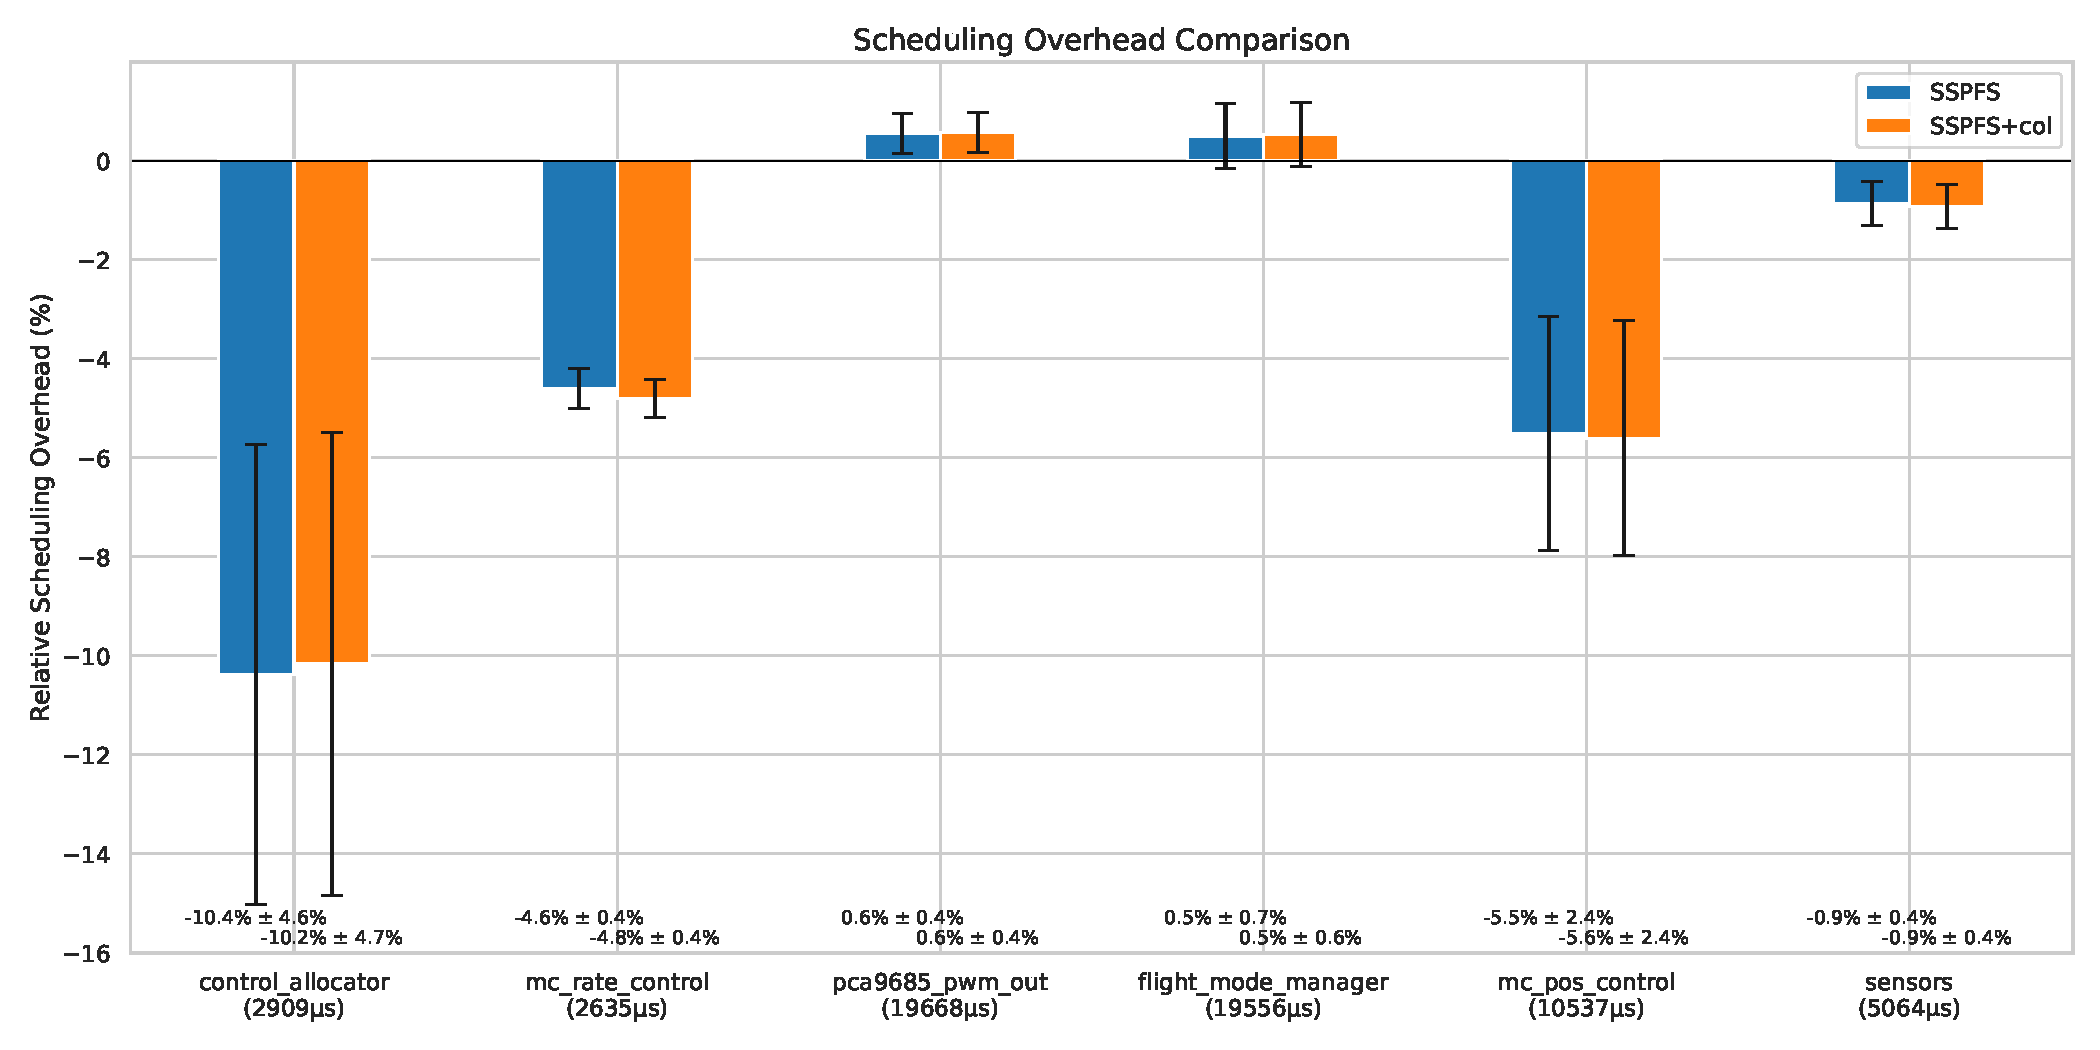
\includegraphics[width=1.0\textwidth]{./img/pdf/px4-sspfs-uspfs} 
  \caption{PX4 tasks scheduling overhead: USPFS vs SSPFS}%
  \label{fig:px4-sspfs-uspfs}
\end{figure}

This performance divergence likely stems from Bao's isolation guarantees: while
\gls{uspfs} processes contend for shared resources, \gls{sspfs} \glspl{vm}
operate within dedicated resource partitions. The cache coloring showed marginal
benefits due to the \gls{uavic}'s \gls{dma} constraints. The \gls{fmu} uses
\gls{spi} sensors that perform \gls{dma} transactions. In turn, the \gls{dma}
requires specific physical memory mapping, which conflicts with coloring's virtual memory
optimizations. Listing~\ref{lst:place-phys} shows the Bao configuration for the
\gls{sspfs} system, where physical memory mapping is enforced by
\lstinline{place_phys = true} assignment.

\begin{longlisting}
\centering
\inputminted[]{bash}{./listing/placePhys.c}
\caption[Physical memory mapping in the SSPFS system]{Physical memory mapping
  in the \gls{sspfs} system: \lstinline{place_phys = true}}
\label{lst:place-phys}
\end{longlisting}

% \paragraph{Video Performance}
Fig.~\ref{fig:cam-sspfs-uspfs} compares the relative \gls{fps} degradation
between systems and analyzes the effect of cache coloring. The results indicate
that the vast majority of runs do not induce any statistically significant
overhead (the whiskers contain 0). On the other hand, runs 10 and 20 exhibit an
outlier behavior, exceeding 30\% in improvement. Once again, the cache coloring
effect is marginal due to the aforementioned \gls{dma} constraints.
These findings align with the previous Companion \gls{vm} benchmarks, confirming
minimal impact on the video surveillance.

\begin{figure}[!hbt]
  \centering
  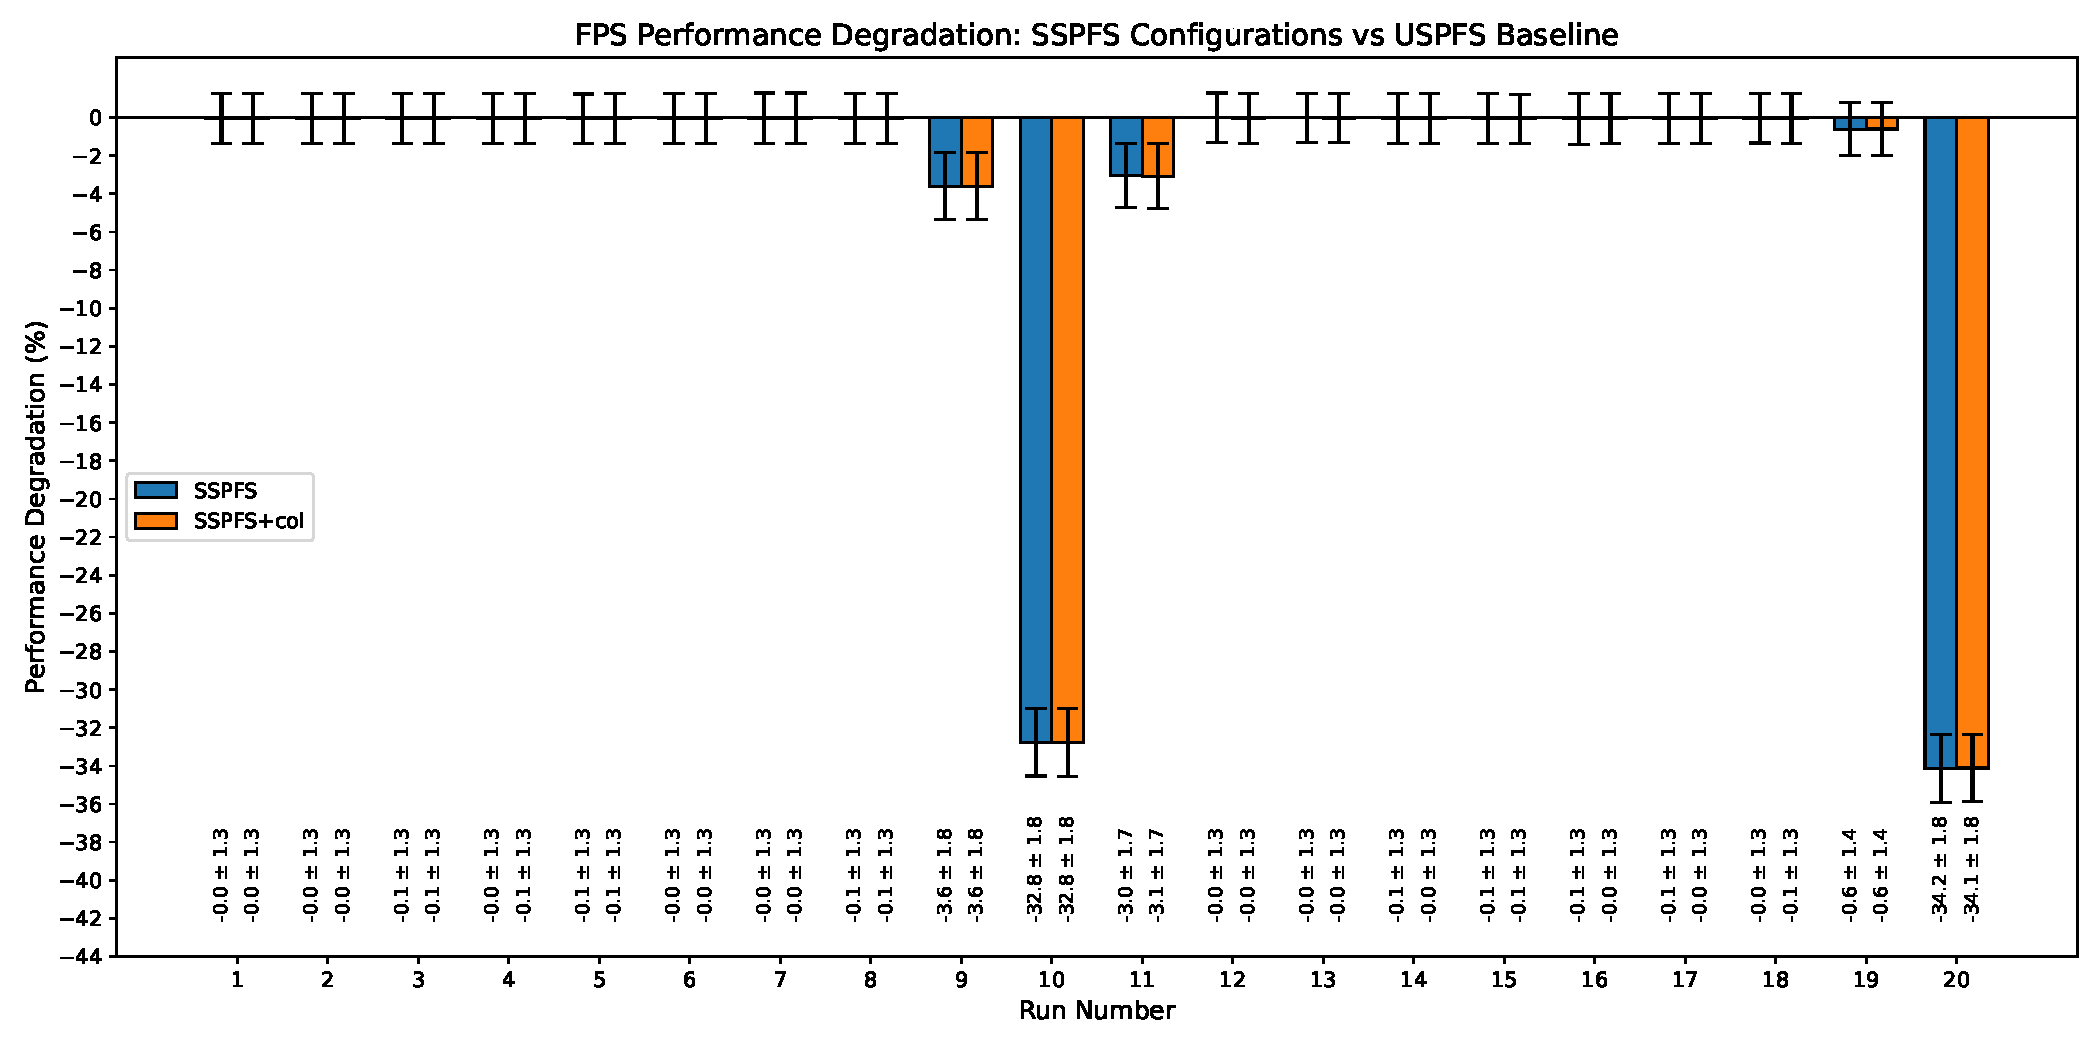
\includegraphics[width=1.0\textwidth]{./img/pdf/cam-sspfs-uspfs} 
  \caption{Relative FPS Performance Degradation: USPFS vs SSPFS}%
  \label{fig:cam-sspfs-uspfs}
\end{figure}

% \paragraph{Conclusion}
Overall, the systems' benchmarking demonstrated that beyond isolation benefits,
the supervised \gls{sspfs} architecture can yield performance advantages in
consolidated mixed-criticality systems.
The static resource partitioning eliminates contention-related overheads
observed in \gls{uspfs}, establishing \gls{sspfs} as the optimal solution for
flight controller and video surveillance integration.

\section{UAV benchmarks}
\label{sec:uav-benchmarks}
Finally, we evaluated both flight stacks under realistic conditions.
For this we configured an automated mission in QGroundControl
(Fig.~\ref{fig:mission-final}), ensuring a repeatable flight profile can be used
to benchmark the \gls{uspfs} and \gls{sspfs} systems in real-flight scenarios.
%
The mission design incorporates two critical geospatial elements. An
external polygon defines the geofence perimeter, which triggers a
return-to-home failsafe if violated. The internal path is the flight path from
takeoff \lstinline{T} to landing \lstinline{L}. At takeoff the \gls{uav} ascends
to an altitude of 2 meters and flies to waypoint \lstinline{3}, then reverses
the direction and heads to \lstinline{4}, and concludes at landing point
\lstinline{L}, maintaining a constant altitude throughout. As it lands, the \gls{uav} decreases speed to enable a safe and smooth landing.


\begin{figure}[!hbt]
  \centering
  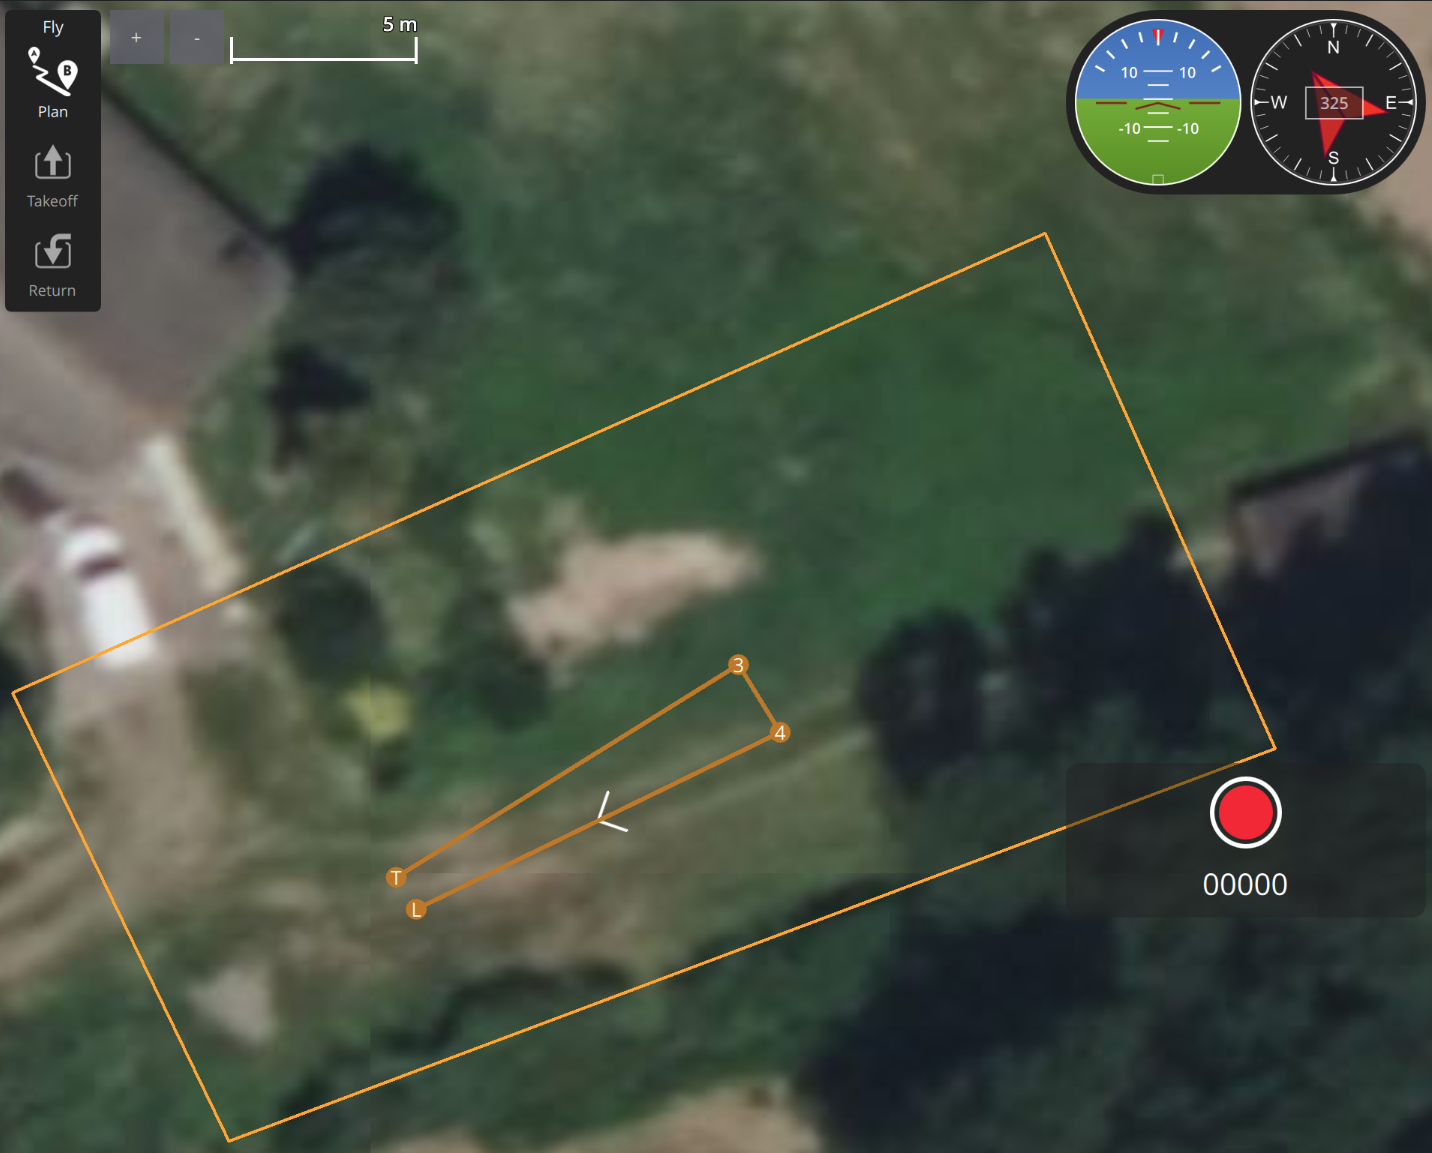
\includegraphics[width=0.7\textwidth]{./img/png/mission-final} 
  \caption{Automated mission configuration in QGroundControl}%
  \label{fig:mission-final}
\end{figure}

We then performed a total of 33 flights per system, conducted under consistent
weather conditions. Each system was tested in a batch as switching
between systems requires significant battery and time resources, preventing
randomized sequencing.
The flight logs were preserved for subsequent analysis of two critical metrics:
(1) position tracking accuracy, and (2) system resource utilization patterns.
We chose the sample size to achieve statistical power to detect meaningful
differences in these operational parameters.
%
The PX4 flight logs are stored as ULog files (\lstinline{.ulg}), containing
\gls{uorb} topic messages subscribed to or published by various
modules. Specifically, we analyzed the \lstinline{vehicle_local} and
\lstinline{vehicle_local_setpoint} topics for position tracking assessment, and
the \lstinline{cpuload} topic to evaluate system resource
utilization.
%
To account for temporal variations between flights, the time domain was
normalized to a mission progress scale $[0, 100]$ using linear interpolation:
\begin{equation}
t_{\text{norm}} = \frac{t - t_{\min}}{t_{\max} - t_{\min}} \times 100
\end{equation}
where $t$ is the original timestamp, and $t_{\min}$ and $t_{\max}$ represent the start and end times of each flight respectively.
%
At each normalized time point $\tau$, the 95\% confidence intervals for group
means were calculated using the Student's $t$-distribution~\cite{t-test}:
\begin{equation}
\text{CI}(\tau) = \bar{x}(\tau) \pm t_{\alpha/2, df} \cdot \frac{s(\tau)}{\sqrt{n(\tau)}}
\end{equation}
where:
\begin{itemize}
    \item $\bar{x}(\tau)$ is the sample mean at progress $\tau$
    \item $s(\tau)$ is the sample standard deviation
    \item $n(\tau)$ is the number of valid observations
    \item $df = n(\tau) - 1$ degrees of freedom
    \item $t_{\alpha/2, df}$ is the critical $t$-value ($\alpha = 0.05$)
\end{itemize}

Statistical significance between systems was evaluated using the two-sided
Welch's unequal variance $t$-test at each mission progress point. This method is
preferred over the $t$-test, as the samples are independent from each other and variance may vary~\cite{welch-t-test}:
\begin{equation}
  \label{eq:welch-t-test}
t(\tau) = \frac{\bar{x}_1(\tau) - \bar{x}_2(\tau)}{\sqrt{\frac{s_1^2(\tau)}{n_1(\tau)} + \frac{s_2^2(\tau)}{n_2(\tau)}}}
\end{equation}
%
The degrees of freedom are calculated using Equation~\ref{eq:welch-t-test-df}~\cite{welch-t-test}:
%
\begin{equation}
  \label{eq:welch-t-test-df}
df(\tau) = \frac{\left( \frac{s_1^2(\tau)}{n_1(\tau)} + \frac{s_2^2(\tau)}{n_2(\tau)} \right)^2}{\frac{s_1^4(\tau)}{n_1^2(\tau)(n_1(\tau)-1)} + \frac{s_2^4(\tau)}{n_2^2(\tau)(n_2(\tau)-1)}}
\end{equation}

The null hypothesis ($H_0$) states no statistical difference between systems:
\begin{equation}
H_0: \mu_{\text{\gls{uspfs}}}(\tau) = \mu_{\text{\gls{sspfs}}}(\tau)
\end{equation}
$H_0$ was rejected at $\alpha = 0.05$ significance level when $p(\tau) <
0.05$. The \lstinline{cmpLogs.py} Python script (see~\cite{thesis-sw-github})
contains the log analysis' implementation details.
%with false discovery rate controlled pointwise across the mission timeline.

Fig.~\ref{fig:mission-exec-sspfs} illustrates the critical phases of a mission
executing in the \gls{sspfs} system, while
Fig.~\ref{fig:mission-final-actual} shows the actual flight path.
Fig.~\ref{fig:mission-exec-case1} depicts the take-off stage alongside the
employed software components, including: (1) QGroundControl for mission flight
management and logging on the host system (2); (3) the \lstinline{gstreamer}
receiver pipeline with its associated \gls{gui} executing on the host (6); the
U-Boot loader, and the \gls{fmu} \gls{vm} console responsible for PX4 execution
(4); the \lstinline{gstreamer} sender pipeline, running on the Companion
\gls{vm} and accessible through a remote \gls{ssh} connection over Wi-Fi.

% Figure environment with subfigures
\begin{figure}[!hbt]
  \centering
  % Row 1: Full width
  \begin{subfigure}[t]{\textwidth}
    \centering
    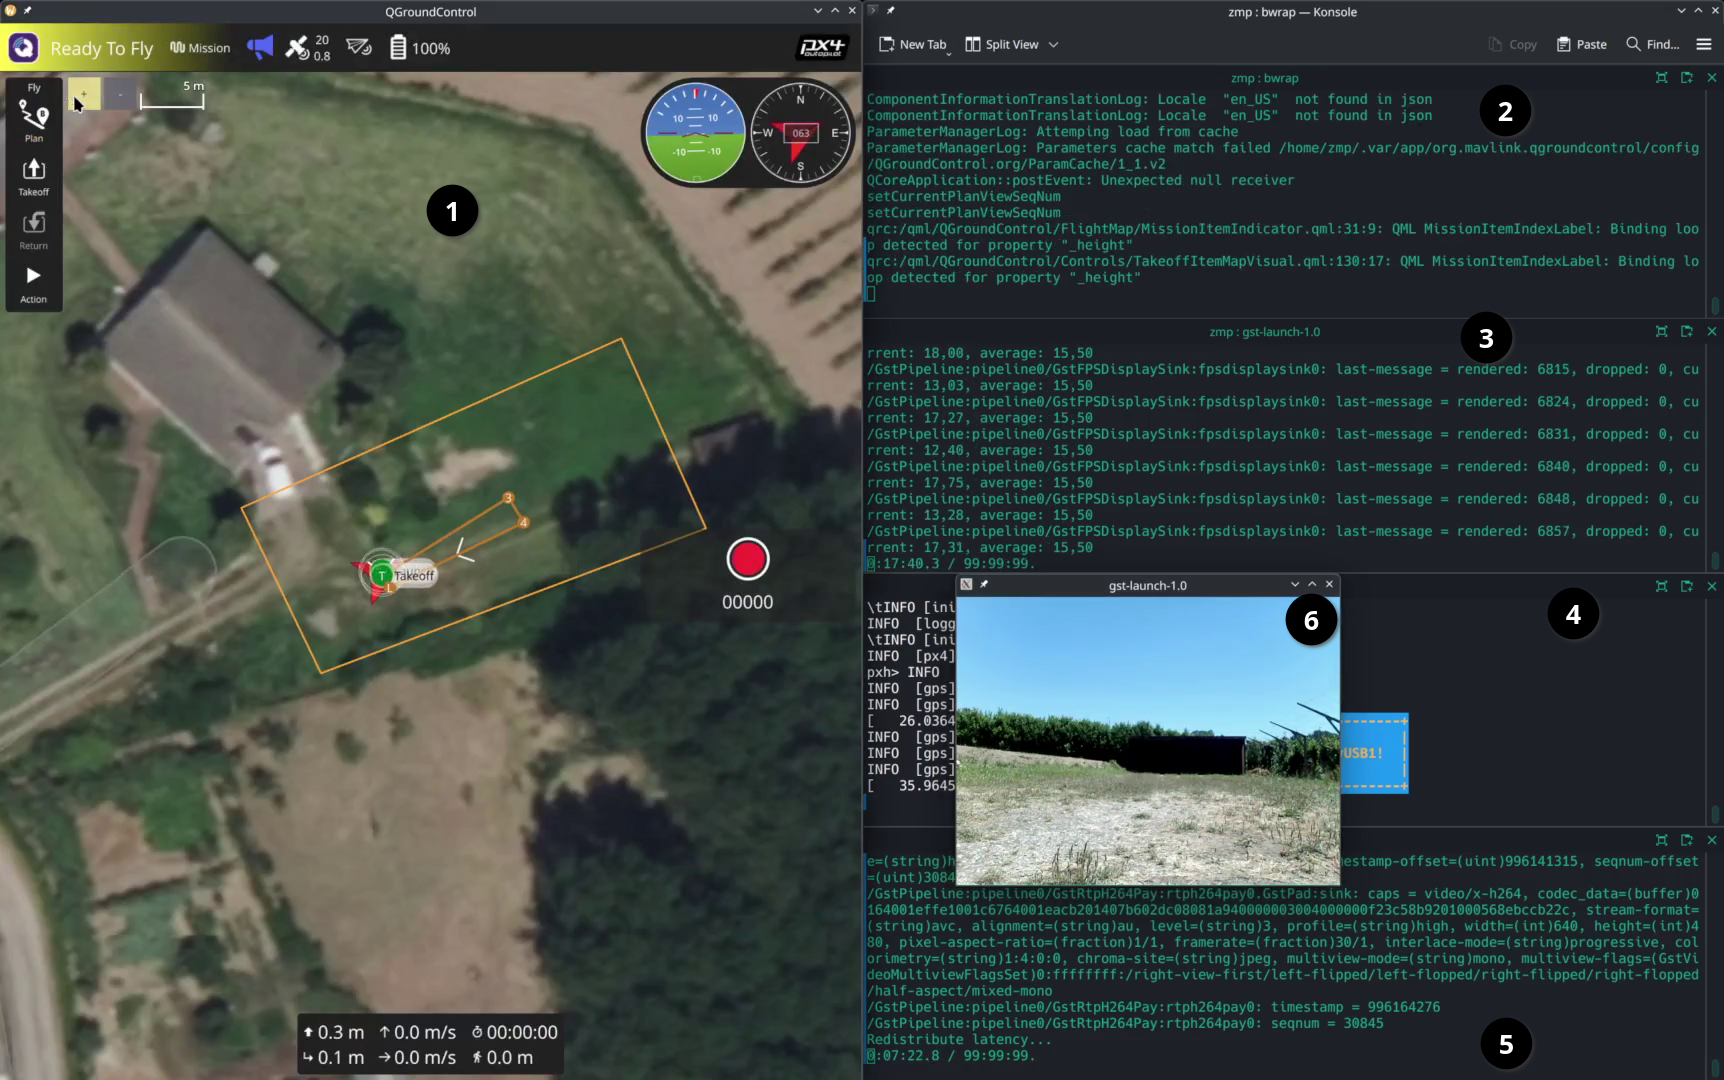
\includegraphics[width=1.0\textwidth]{./img/png/bao-fpv-takeoff-annot} 
    \caption{Take-off}%
    \label{fig:mission-exec-case1}
  \end{subfigure}
%  \\[0.5\baselineskip] % Vertical space after first row
  
  % Row 2: Two half-width images
  \begin{subfigure}[t]{0.49\textwidth}
    \centering
    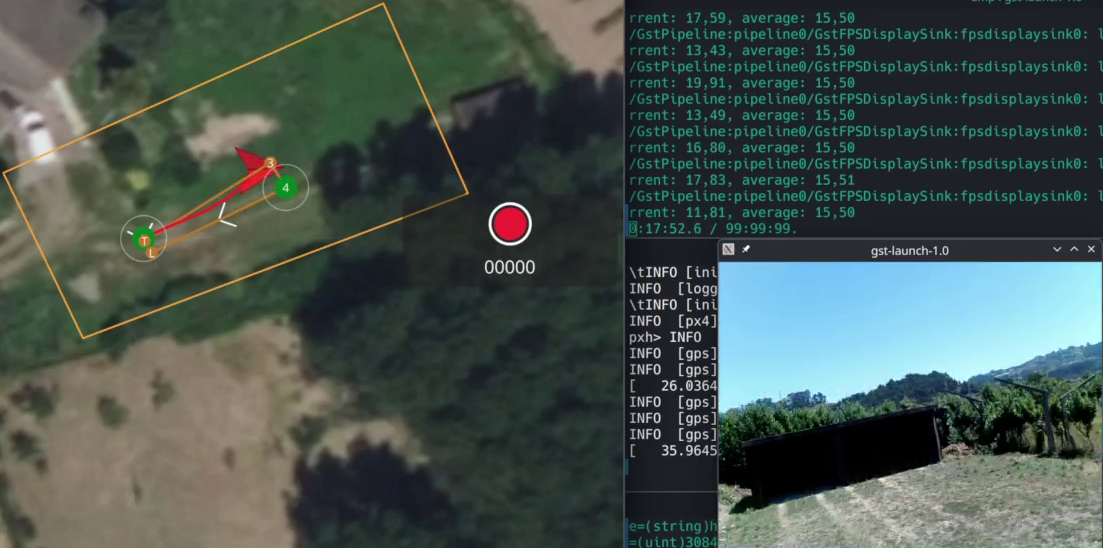
\includegraphics[width=\linewidth]{./img/png/bao-fpv-3-annot} % Use \linewidth inside subfigure
    \caption{Point 3}%
    \label{fig:mission-exec-case2}
  \end{subfigure}
  \hfill % Horizontal filler
  \begin{subfigure}[t]{0.49\textwidth}
    \centering
    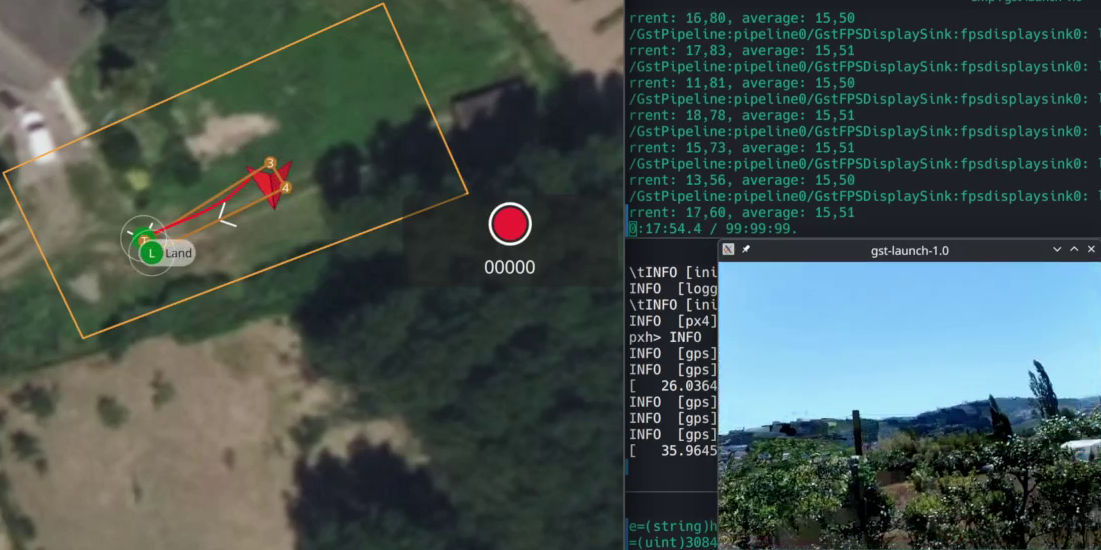
\includegraphics[width=\linewidth]{./img/png/bao-fpv-4-annot} 
    \caption{Point 4}%
    \label{fig:mission-exec-case3}
  \end{subfigure}
%  \\[0.5\baselineskip] % Vertical space after second row
  
  % Row 3: Two half-width images
  \begin{subfigure}[t]{0.49\textwidth}
    \centering
    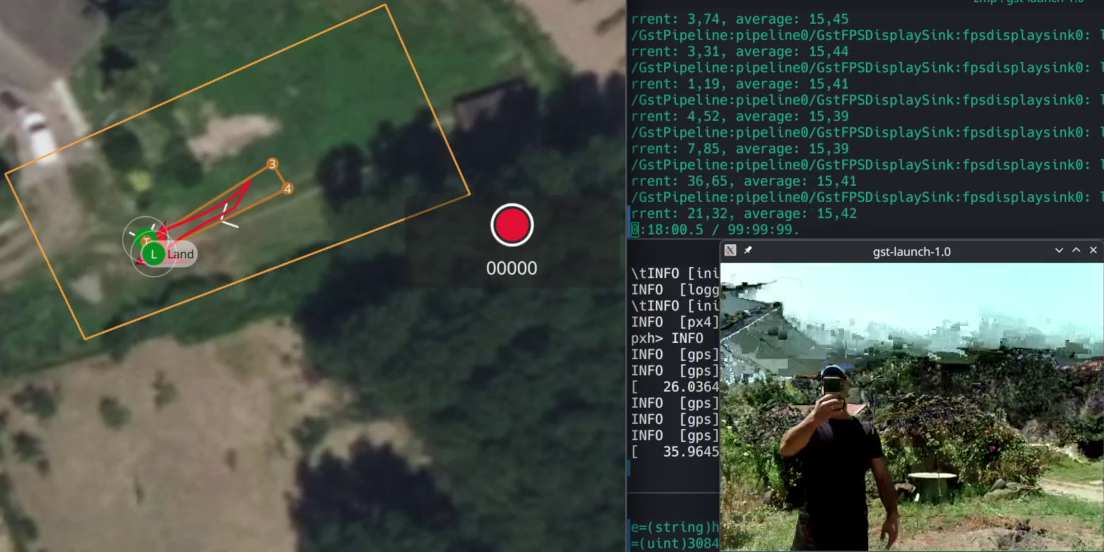
\includegraphics[width=\linewidth]{./img/png/bao-fpv-land-annot} 
    \caption{Landing}%
    \label{fig:mission-exec-case4}
  \end{subfigure}
  \hfill % Horizontal filler
  \begin{subfigure}[t]{0.49\textwidth}
    \centering
    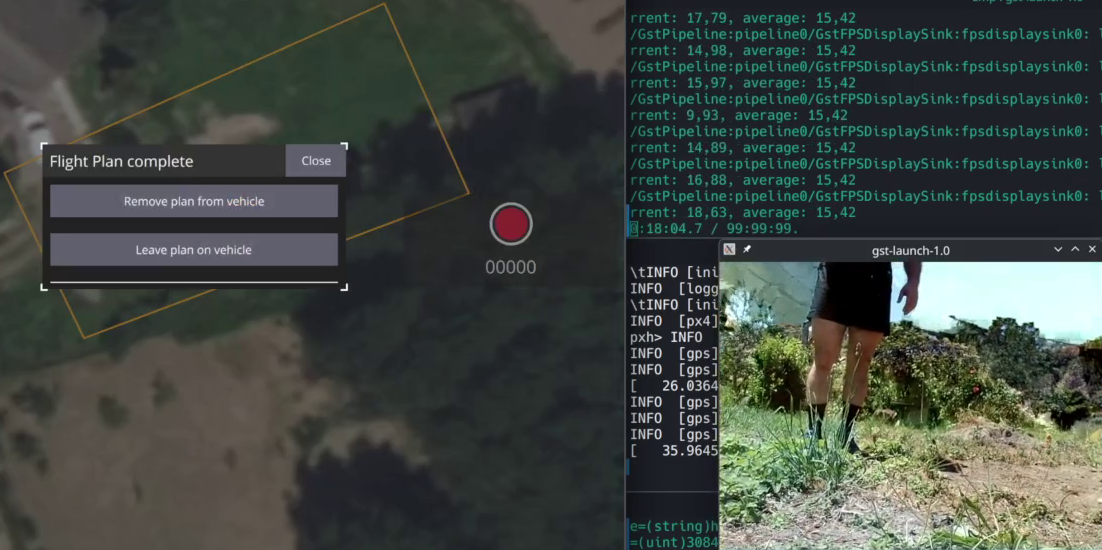
\includegraphics[width=\linewidth]{./img/png/bao-fpv-complete-annot} 
    \caption{Complete}%
    \label{fig:mission-exec-case5}
  \end{subfigure}
  
  \caption{Mission execution -- SSPFS case}
  \label{fig:mission-exec-sspfs}
\end{figure}

Fig.~\ref{fig:mission-exec-case2} and Fig.~\ref{fig:mission-exec-case3}
show the flight path progression through the intermediate waypoints and the
corresponding video streaming.
Fig.~\ref{fig:mission-exec-case3} demonstrates the landing stage, showing the
\gls{uav} operator, and shortly after the mission is completed successfully (Fig.~\ref{fig:mission-exec-case4}).
%
These results confirm that the \gls{sspfs} system functions as designed: the
autopilot operates within the \gls{fmu} \gls{vm}, exchanging data with the
\gls{gcs} through the telemetry radio link, while video streaming executes on
the \lstinline{Companion} \gls{vm}, capturing live feed from the \gls{usb} camera and transmitting it over Wi-Fi.

To interpret the test results we must analyze the actual mission flight path,
illustrated as a red line in Fig.~\ref{fig:mission-final-actual}.
Mission paths exhibit slight variations due to differing sensor estimates and
weather conditions.
%
As anticipated, the autopilot dynamically adjusts trajectories according to
vehicle flight dynamics and parameters rather than strictly following predefined
paths. This adaptation is particularly evident during the sharp turn between
points \lstinline{3} and \lstinline{4}.
%
Consequently, although PX4 tries to adapts the trajectory to follow smooth
curves (defined by the acceptance radius parameter
(\lstinline{NAV_ACC_RAD})~\cite{px4MissionModePath}), the velocity modulation
during approach and departure phases may limit this, based on the jerk-limiting tuning parameters.

\begin{figure}[!hbt]
  \centering
  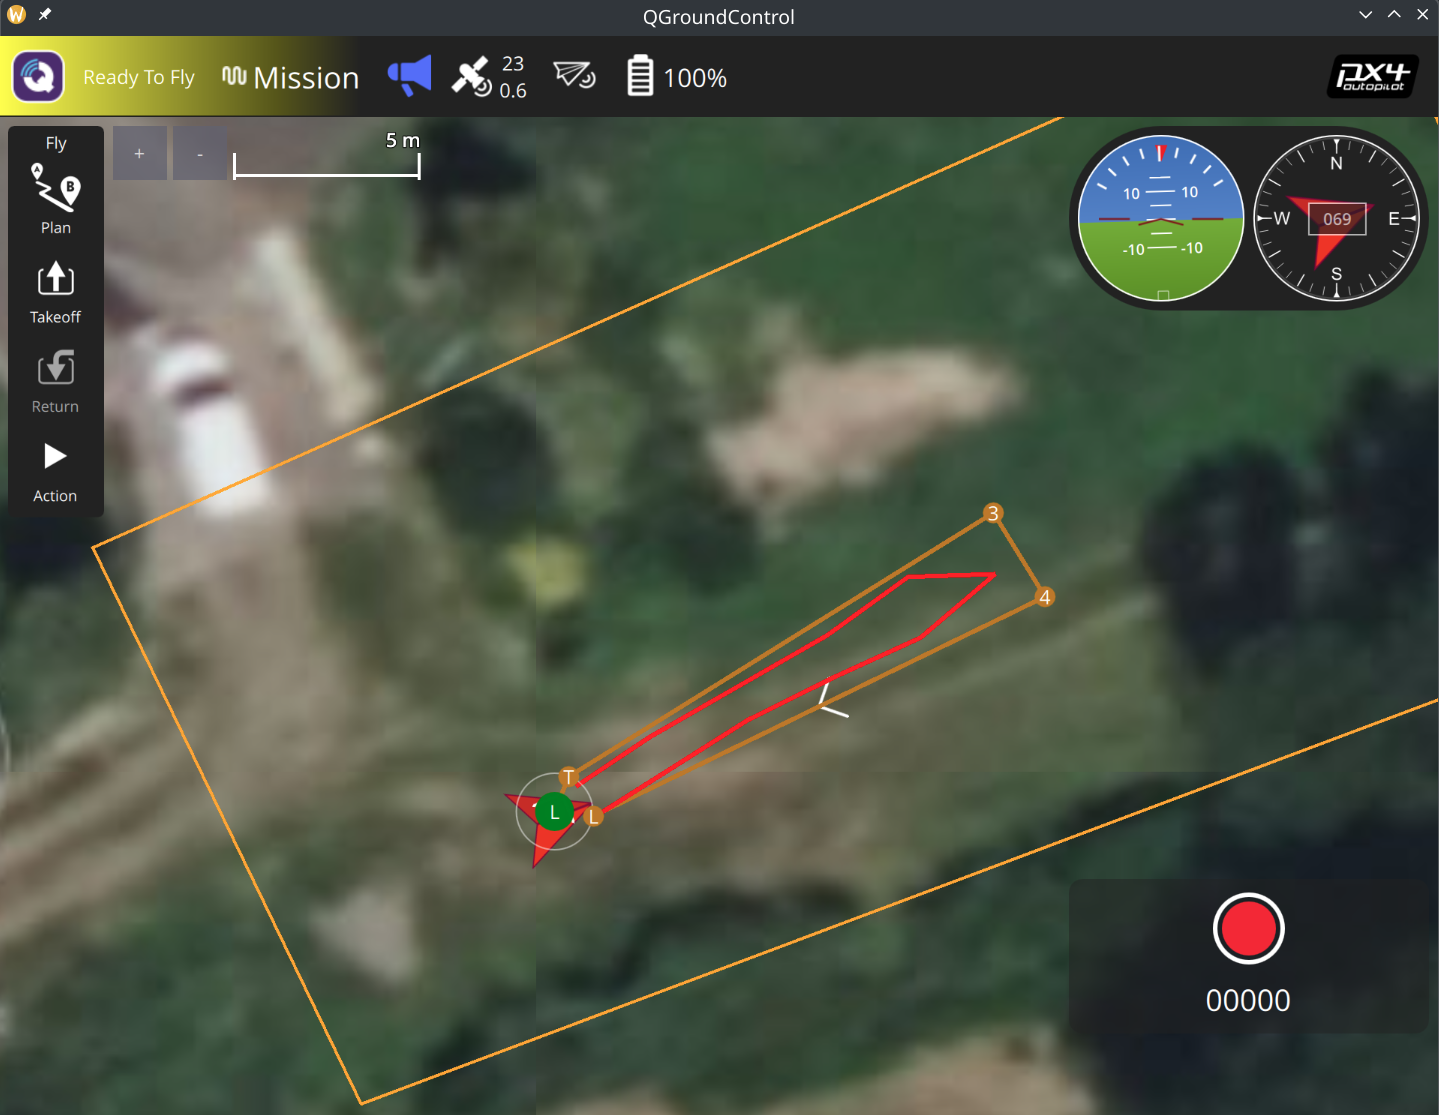
\includegraphics[width=0.8\textwidth]{./img/png/mission-final-actual} 
  \caption{Actual flight path of a mission in QGroundControl}%
  \label{fig:mission-final-actual}
\end{figure}

Fig.~\ref{fig:pos-track-cmp} presents the comparison in position 
tracking performance between the \gls{uspfs} and \gls{sspfs}
systems across X, Y, and Z axes.
%
The solid lines indicate the actual trajectories, while the dotted ones
represent the setpoint trajectories. The blue and orange traces correspond to
the \gls{uspfs} and \gls{sspfs} systems respectively, with the shaded
bands denoting the 95\% confidence intervals for the mean.
%
The controller demonstrates accurate position tracking, with the observed
trajectories closely following setpoints except during take-off and landing
phases due to flight dynamics.
%
Notably, setpoint variations occur between systems despite identical
missions. This can be attributed to differing flight dynamics influenced by
environmental factors, particularly air pressure variations affecting Z-axis
estimates~\cite{px4-static-pressure,px4-static-pressure-correc}, and sensor
estimation discrepancies, such as noise, e.g. in the \gls{gps} measurements.
%
The significant overlap between the actual and setpoint bands indicates no statistical difference in X and Z-axis
tracking between systems. However, a consistent Y-axis offset of approximately 2
meters is observed. We need to collect more data to investigate the causing factors for
this deviation. Nonetheless, the introduction of supervision in the autopilot
demonstrated no adverse impact on overall position tracking performance.

\begin{figure}[!hbt]
  \centering
  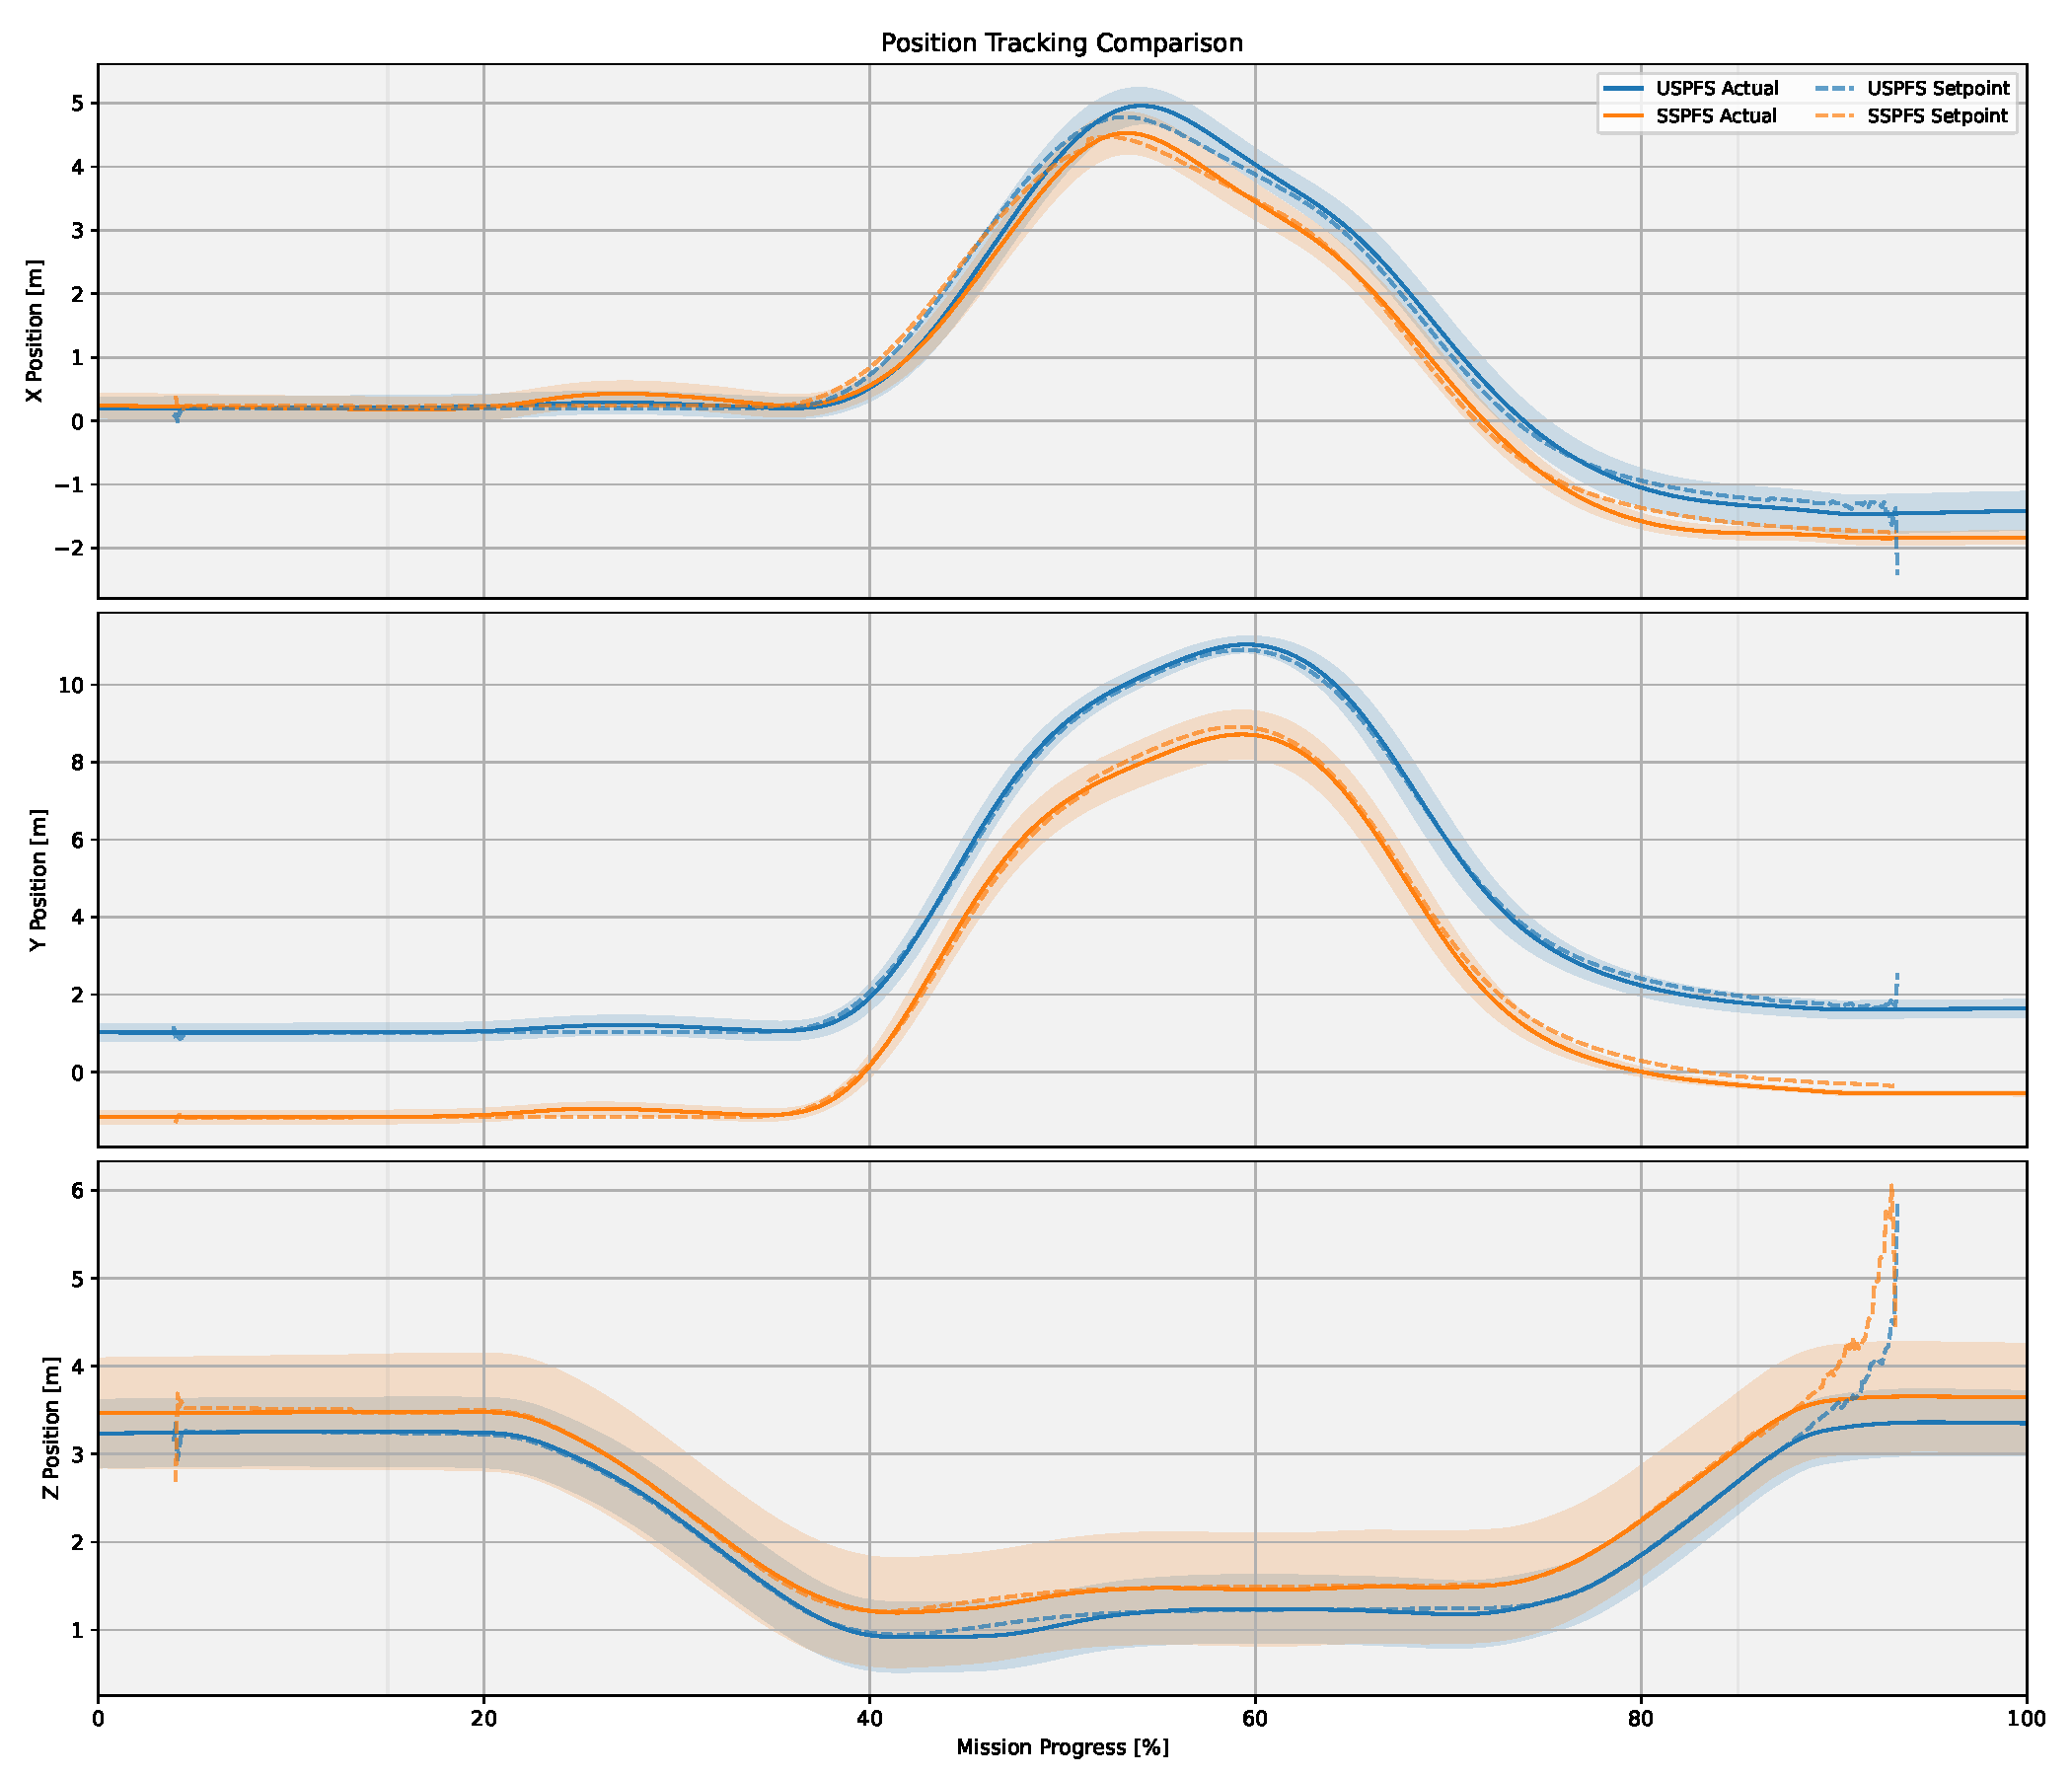
\includegraphics[width=1.0\textwidth]{./img/pdf/pos-track-cmp} 
  \caption{Position tracking comparison between USPFS and SSPFS systems}%
  \label{fig:pos-track-cmp}
\end{figure}

We compared system resource usage between the \gls{uspfs} and \gls{sspfs}
systems, analyzing the PX4 \gls{uorb} messages rather than performing direct
system measurements (Fig.~\ref{fig:sys-resources-cmp}).
The supervised system introduces measurable overhead: 6\% increase in \gls{cpu}
load and 9-fold \gls{ram} utilization growth. \gls{cpu}
results align with prior Bao benchmarks (Section~\ref{sec:bao-benchmarks}),
while \gls{ram} expansion may stem from firmware mailbox supervision requiring
Bao's mailbox manager to intercept transactions.
However, this \gls{ram} increase remains negligible given the \gls{fmu}
\gls{vm}'s 144 MB allocation and the fact the \gls{sspfs} uses about 90 KB of \gls{ram}
instead of the 10 KB from the \gls{uspfs} system.

\begin{figure}[!hbt]
  \centering
  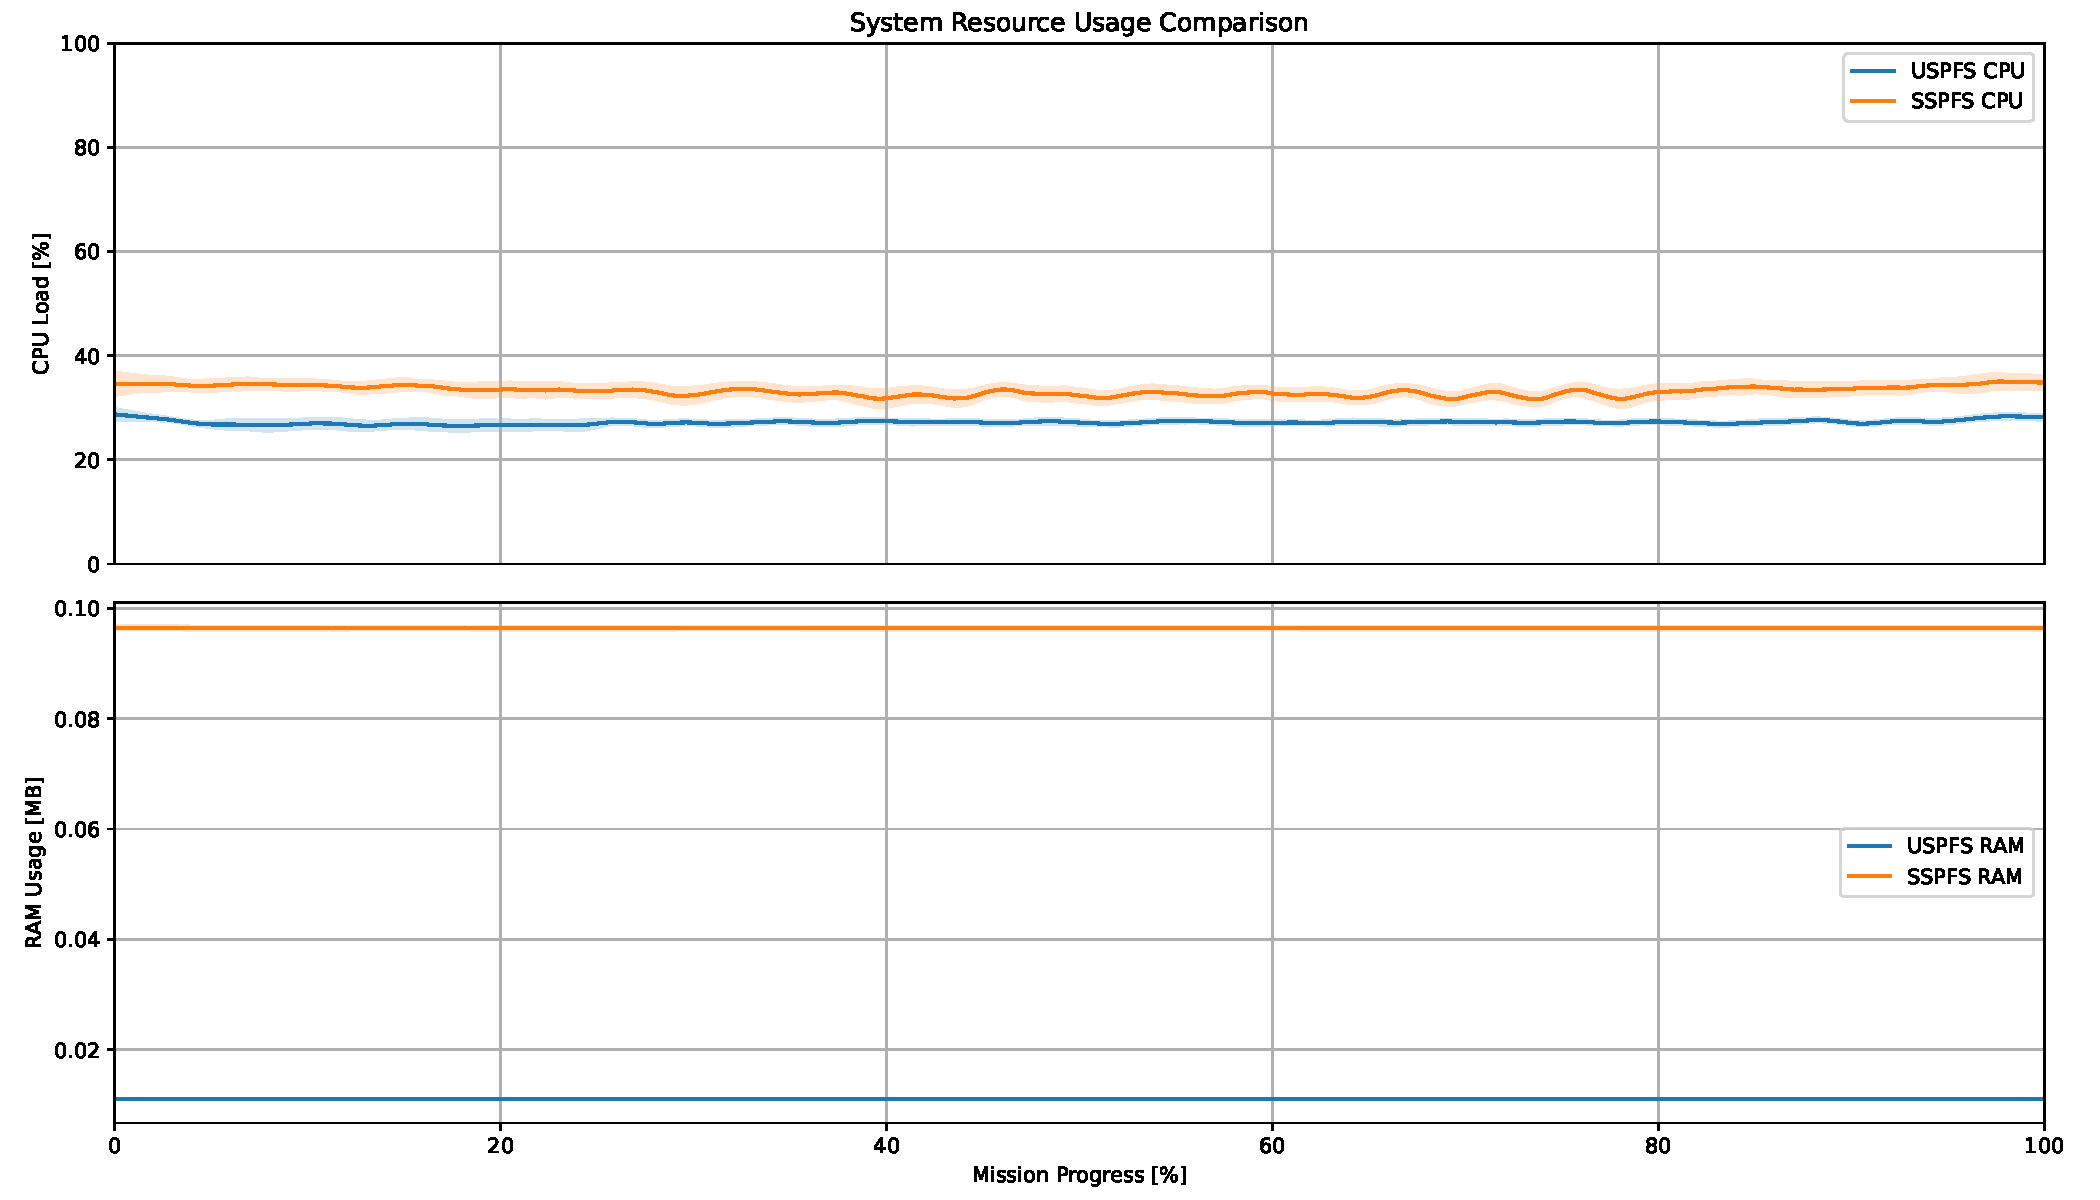
\includegraphics[width=1.0\textwidth]{./img/pdf/sys-resources-cmp} 
  \caption{System resource usage comparison between USPFS and SSPFS systems}%
  \label{fig:sys-resources-cmp}
\end{figure}

The functional tests were replicated in real-flight scenarios. They are fully
detailed in videos available in the online repository~\cite{thesis-sw-github}.
Fig.~\ref{fig:mission-exec-sspfs-last} demonstrates the \gls{sspfs} system behavior
during a system compromise. Fig.~\ref{fig:mission-exec-sspfs-takeoff-1} shows
the software tools used and the \gls{uav}'s flight view: (1) QGroundControl
mission planning and tracking; (2) \lstinline{gstreamer} receiver pipeline
running at the \gls{gcs} and its \gls{gui} (6); telemetry-data collected by PX4
and accessible through QGroundControl (3); (4) U-Boot loader and
\gls{fmu} \gls{vm} executing PX4; (5) \lstinline{Companion}
\gls{vm} running the \lstinline{gstreamer} sender pipeline and accessible via
\gls{ssh} over Wi-Fi; (7) and remote \gls{ssh} shell to compromise the Companion
\gls{vm}. We can observe that the video streaming is operating normally during
takeoff and that the \gls{uav} starts to fly (Fig.~\ref{fig:mission-exec-sspfs-takeoff-2}).
We then executed the malicious kernel module within the \lstinline{Companion}
\gls{vm}. Video streaming immediately freezed, indicating compromised
functionality in this \gls{vm}. Despite this failure, the \gls{uav} lands (Fig.~\ref{fig:mission-exec-sspfs-final}),
indicating that PX4 remained fully operational and, thus, the mission is completed successfully.
%
These results demonstrate Bao's hypervisor capability to effectively isolate the
critical flight stack (\gls{fmu} \gls{vm}) from non-critical components
(\lstinline{Companion} \gls{vm}).
Consequently, crashes in the \lstinline{Companion} \gls{vm} remain contained without propagating to the autopilot, thereby preventing potential catastrophic \gls{uav} failure.

\begin{figure}[!hbt]
  \centering
  % Row 1: Full width
  \begin{subfigure}[t]{\textwidth}
    \centering
    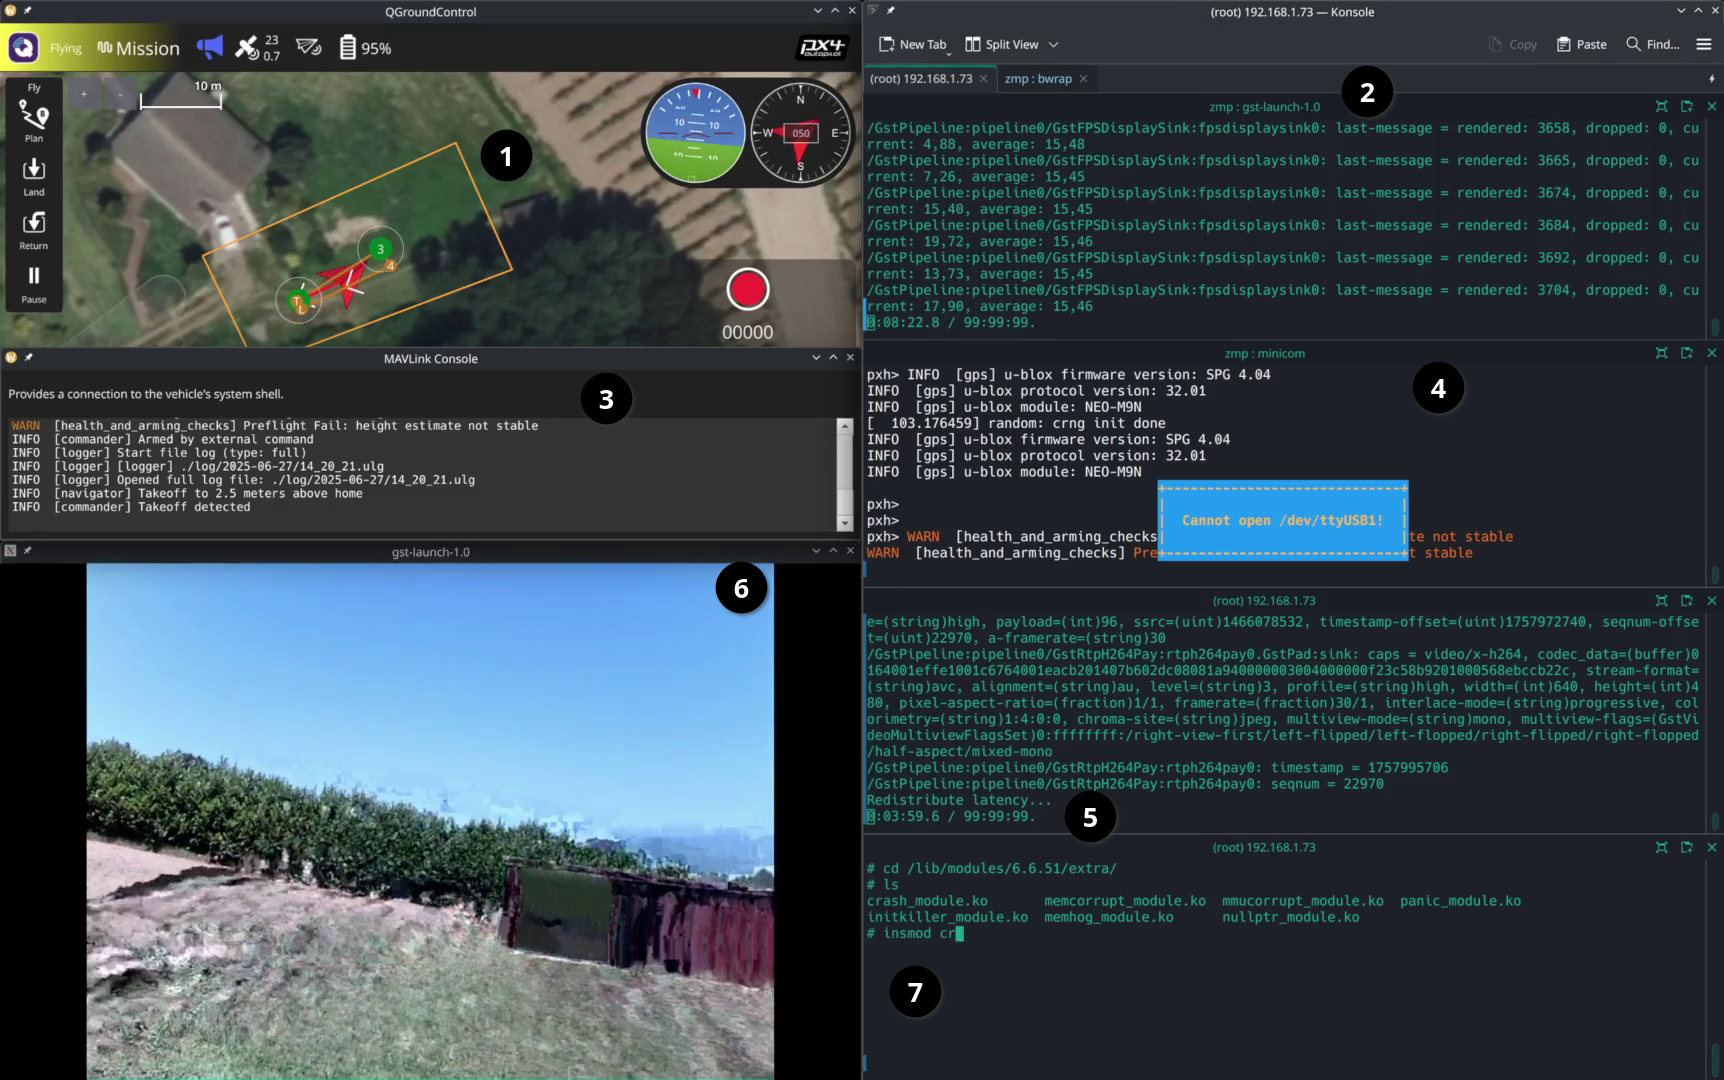
\includegraphics[width=1.0\textwidth]{./img/png/bao-fpv-insmod-1} 
    \caption{UAV's view: takeoff}%
    \label{fig:mission-exec-sspfs-takeoff-1}
  \end{subfigure}
%  
  % Row 2: Two half-width images
  \begin{subfigure}[t]{0.49\textwidth}
    \centering
    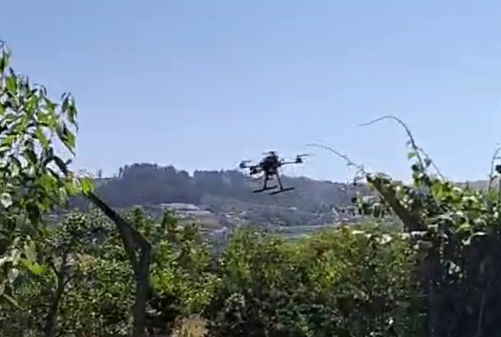
\includegraphics[width=\linewidth]{./img/png/bao-flight-myView-takeoff} % Use \linewidth inside subfigure
    \caption{Operator's view: takeoff}%
    \label{fig:mission-exec-sspfs-takeoff-2}
  \end{subfigure}
  \begin{subfigure}[t]{0.49\textwidth}
    \centering
    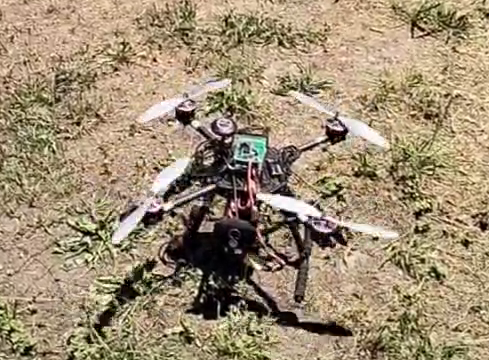
\includegraphics[width=0.92\linewidth]{./img/png/bao-flight-myView-final} % Use \linewidth inside subfigure
    \caption{Operator's view: successful landing}%
    \label{fig:mission-exec-sspfs-final}
  \end{subfigure}
%  
  \caption{Mission execution: functional test (SSPFS)}
  \label{fig:mission-exec-sspfs-last}
\end{figure}
  
% \begin{figure}[!hbt]
%     \centering
%     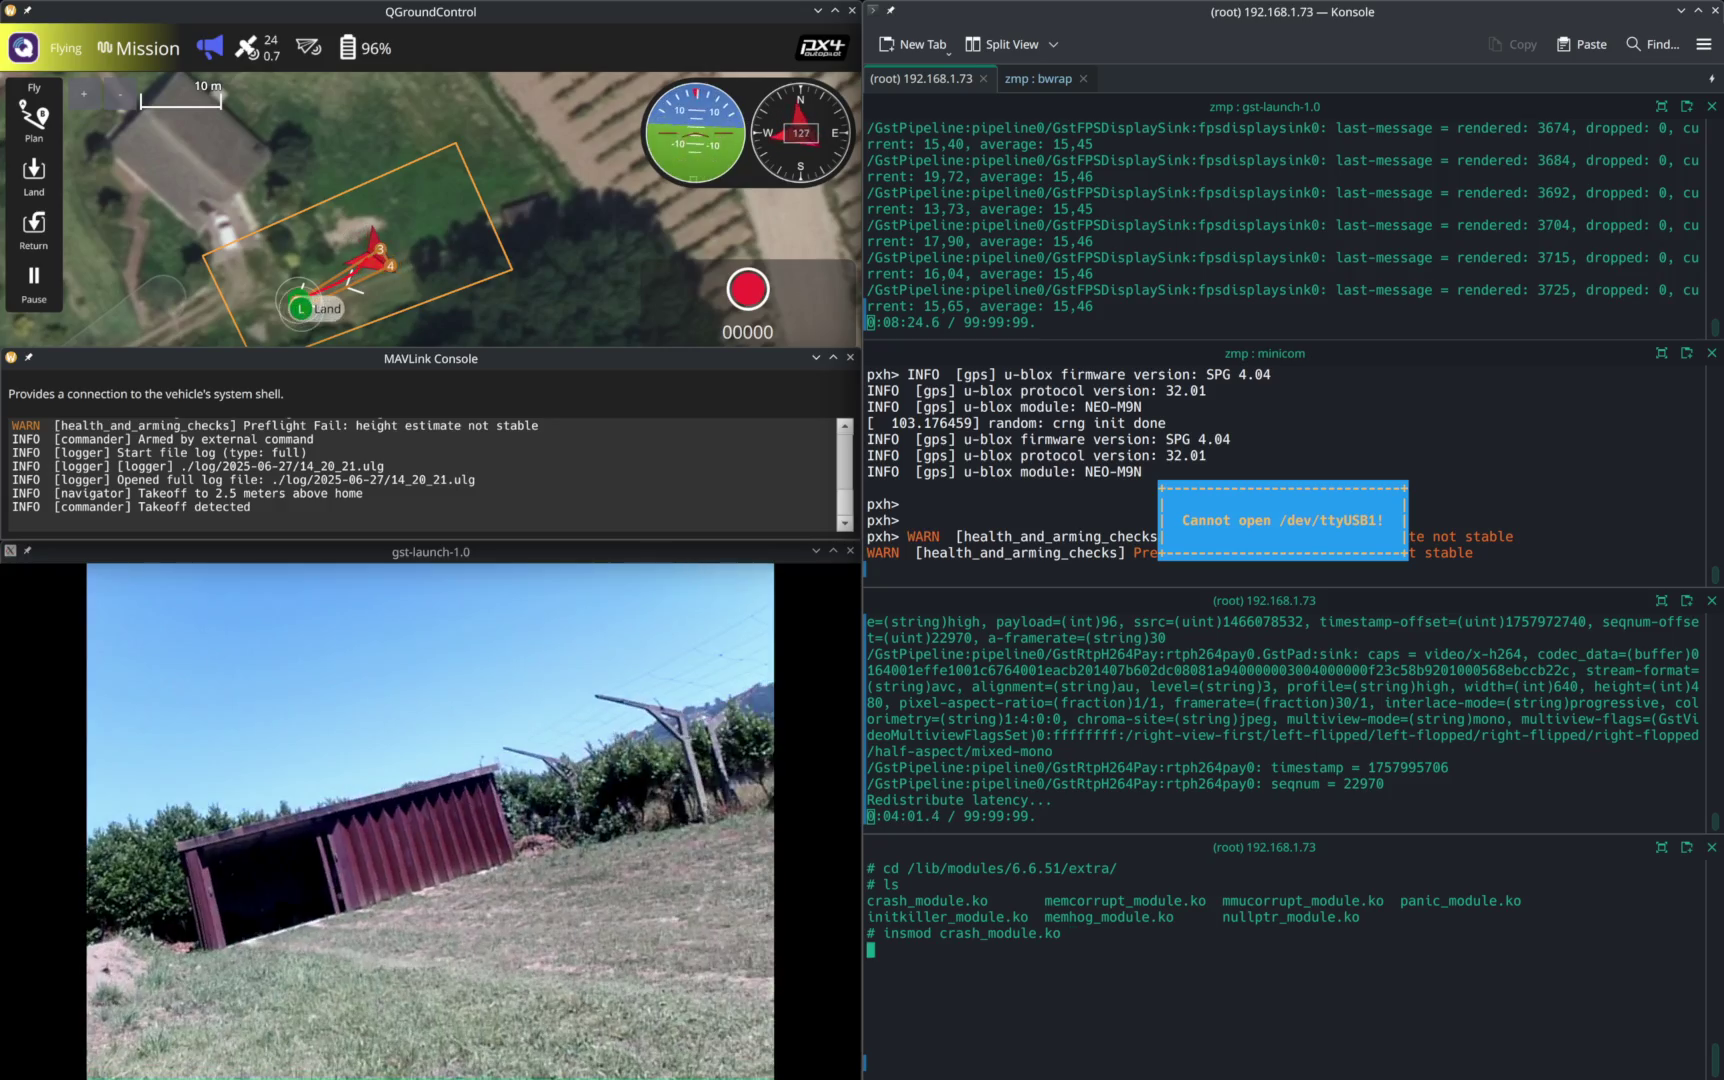
\includegraphics[width=0.9\textwidth]{./img/png/bao-fpv-insmod-2} 
%     \caption{Mission execution: Functional test (SSPFS) -- running a malicious kernel module}%
%     \label{fig:mission-exec-insmod-2}
%   \end{figure}

% \begin{figure}[!hbt]
%   \centering
%   % Row 1: Full width
%   \begin{subfigure}[t]{\textwidth}
%     \centering
%     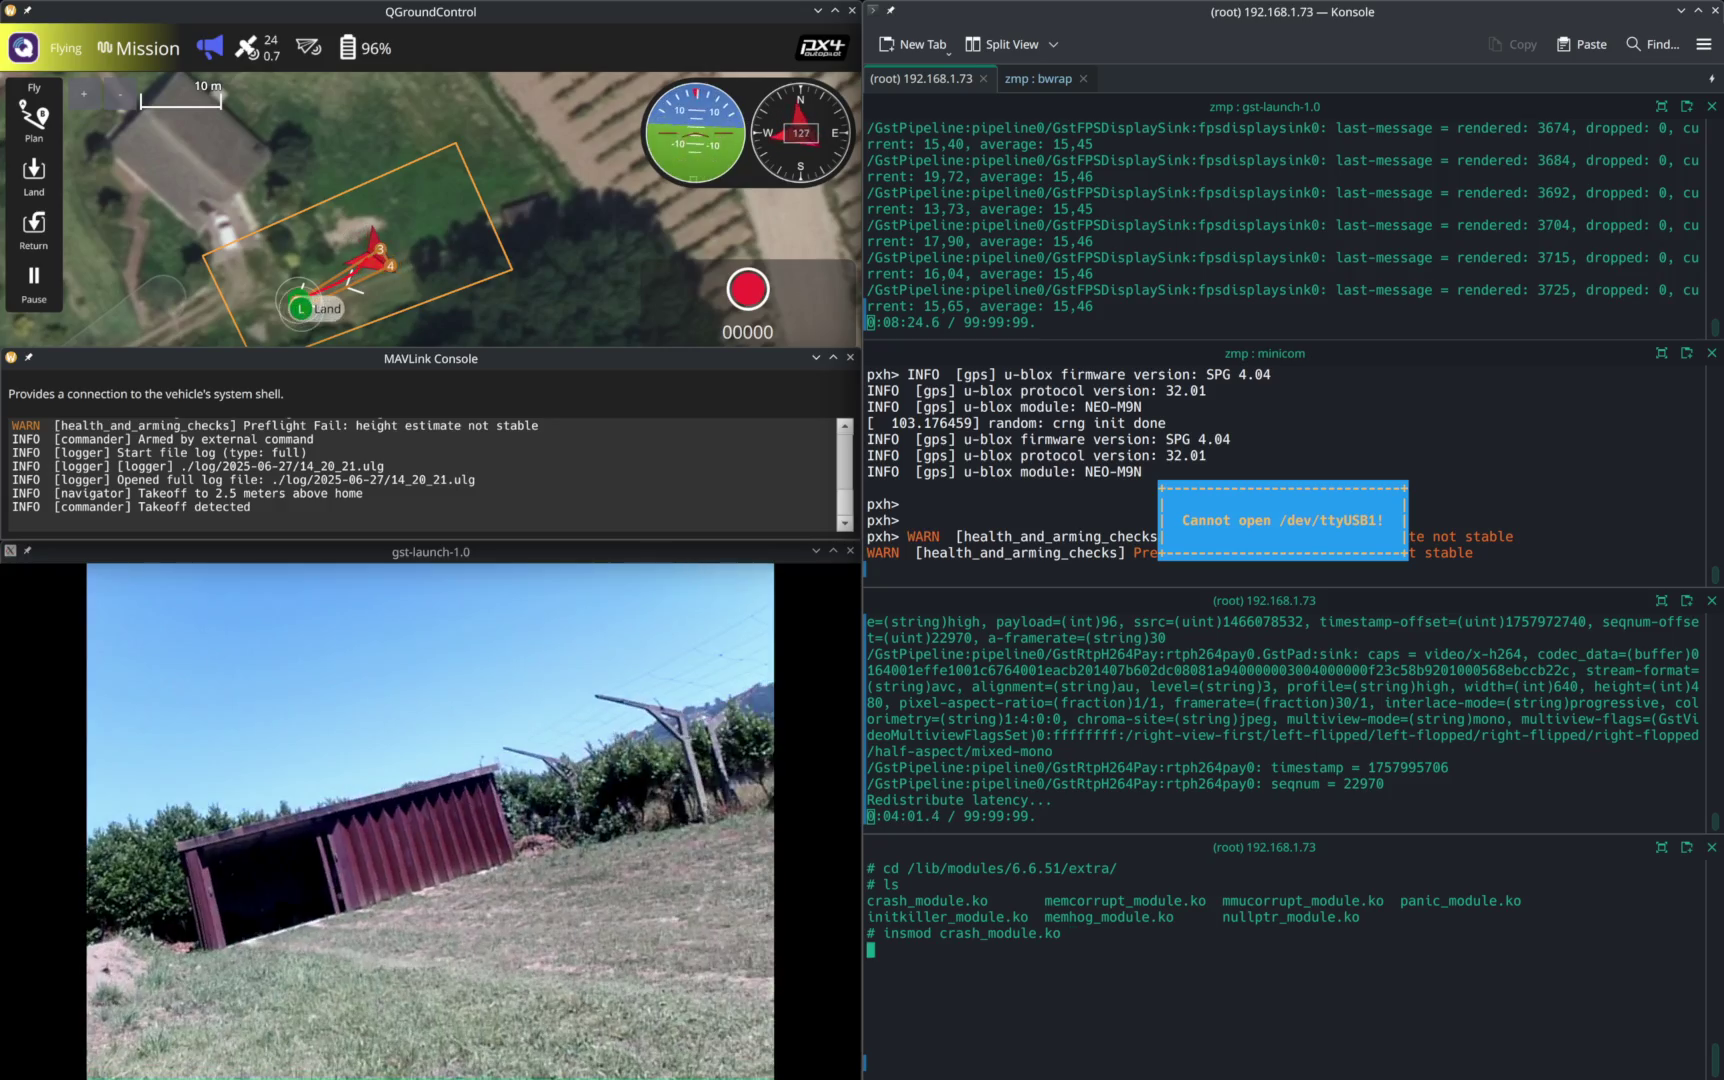
\includegraphics[width=1.0\textwidth]{./img/png/bao-fpv-insmod-2} 
%     \caption{UAV's view}%
%     \label{fig:mission-exec-insmod-1}
%   \end{subfigure}
% %  
%   % Row 2: Two half-width images
%   \begin{subfigure}[t]{0.49\textwidth}
%     \centering
%     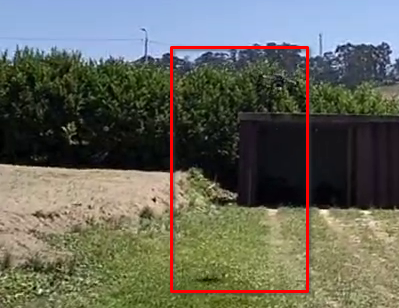
\includegraphics[width=\linewidth]{./img/png/bao-flight-myView-insmod} % Use \linewidth inside subfigure
%     \caption{Operator's view}%
%     \label{fig:mission-exec-insmod-2}
%   \end{subfigure}
% %  
%   \caption{Mission execution: Functional test (SSPFS) -- executing a malicious
%     kernel module}
%   \label{fig:mission-exec-insmod}
% \end{figure}
  
% \begin{figure}[!hbt]
%     \centering
%     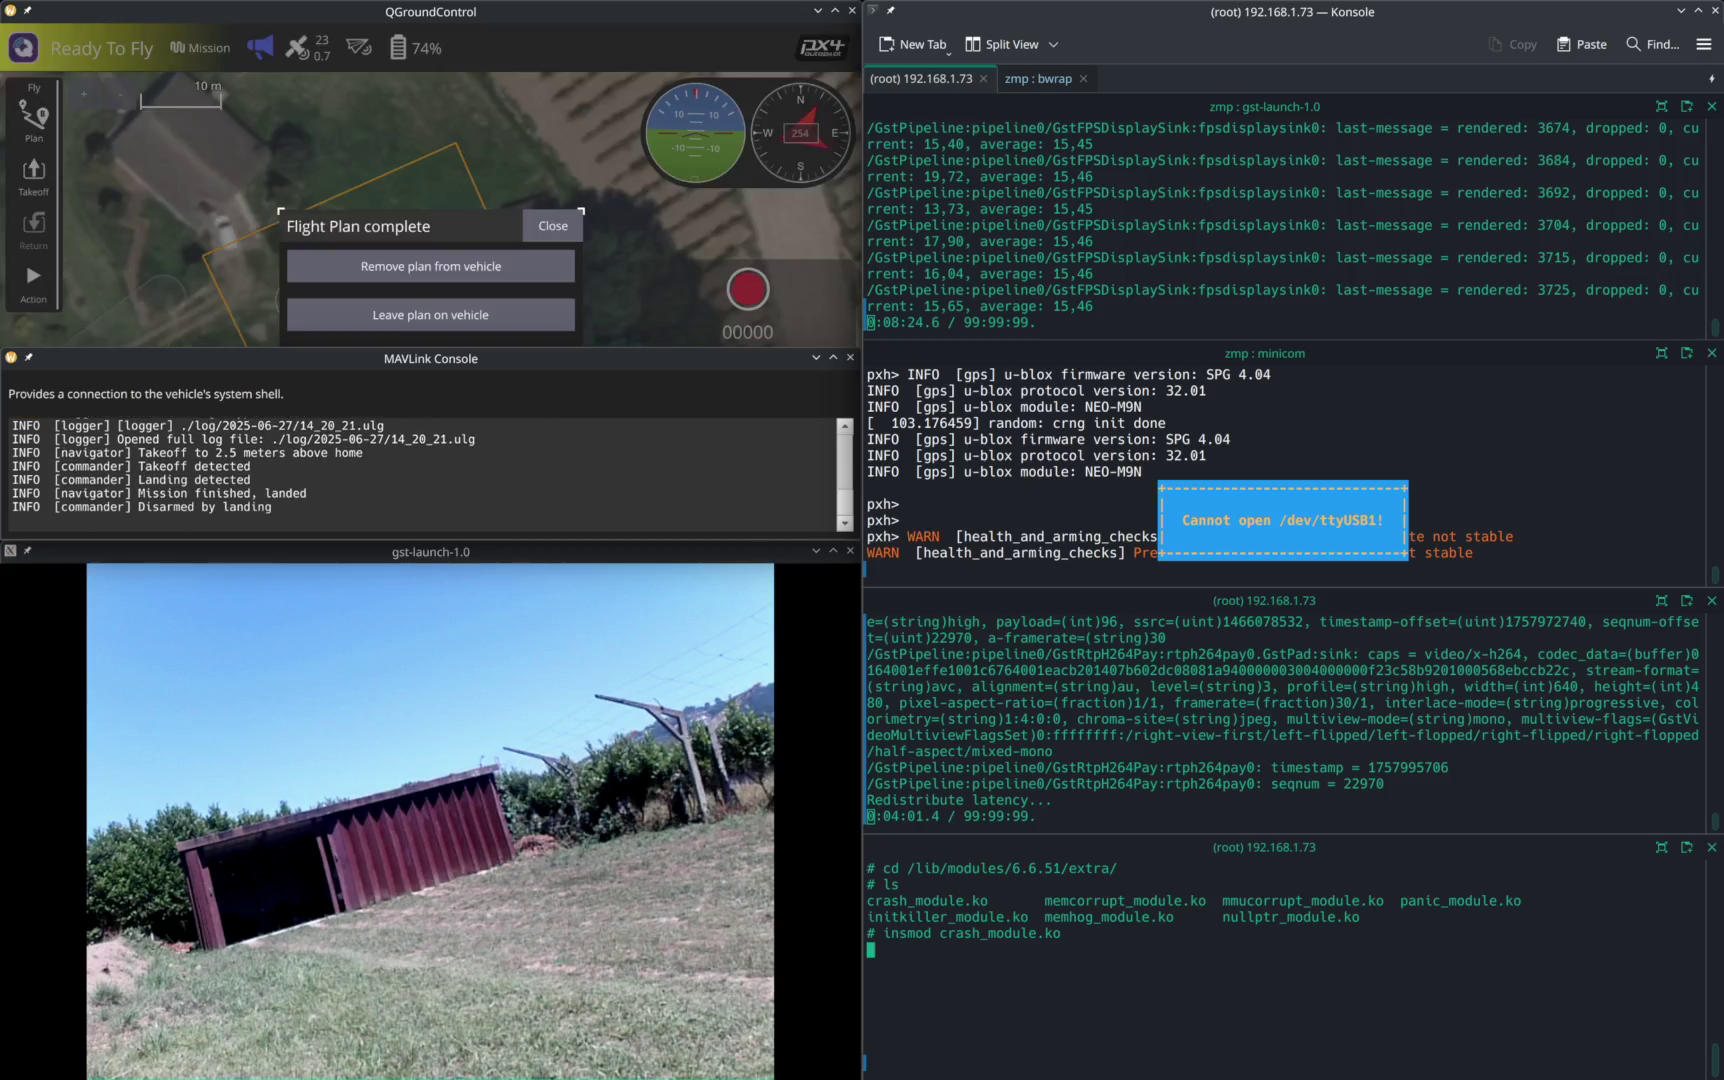
\includegraphics[width=0.9\textwidth]{./img/png/bao-fpv-insmod-3} 
%     \caption{Mission execution: Functional test (SSPFS) -- Mission complete}
%     \label{fig:mission-exec-insmod-3}
%   \end{figure}

% \begin{figure}[!hbt]
%   \centering
%   % Row 1: Full width
%   \begin{subfigure}[t]{\textwidth}
%     \centering
%     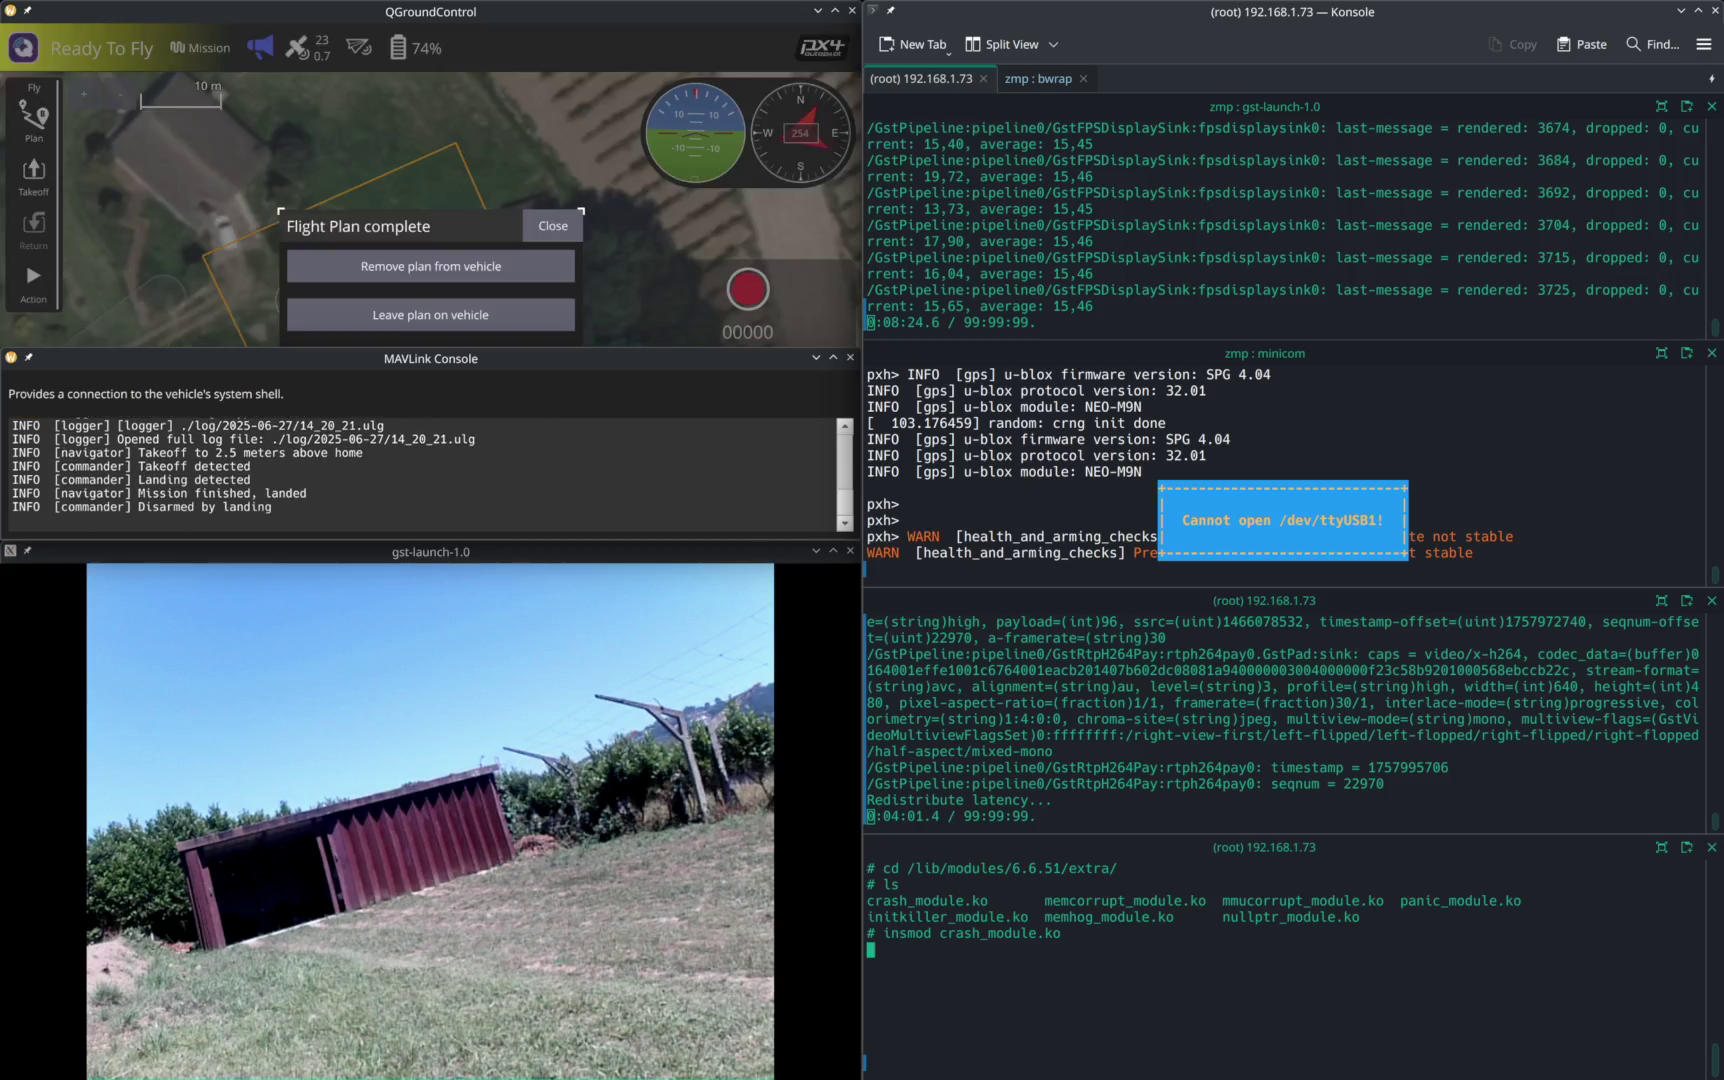
\includegraphics[width=1.0\textwidth]{./img/png/bao-fpv-insmod-3} 
%     \caption{UAV's view}%
%     \label{fig:mission-exec-final-1}
%   \end{subfigure}
% %  
%   % Row 2: Two half-width images
%   \begin{subfigure}[t]{0.49\textwidth}
%     \centering
%     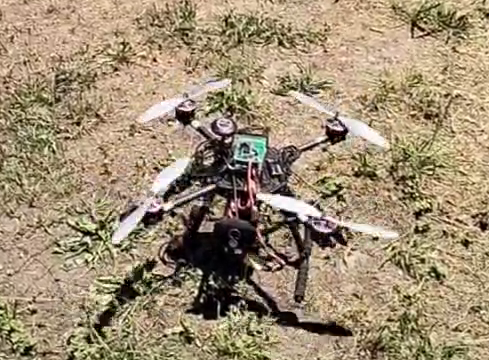
\includegraphics[width=\linewidth]{./img/png/bao-flight-myView-final} % Use \linewidth inside subfigure
%     \caption{Operator's view}%
%     \label{fig:mission-exec-final-2}
%   \end{subfigure}
% %  
%   \caption{Mission execution: Functional test (SSPFS) -- mission complete}
%   \label{fig:mission-exec-final}
% \end{figure}

The same functional test procedure was subsequently applied to the \gls{uspfs}
system.
Fig.~\ref{fig:mission-exec-uspfs} demonstrates the \gls{uspfs} system behavior
during a system compromise. Fig.~\ref{fig:mission-exec-uspfs-takeoff-1} shows
the software tools used and the \gls{uav}'s flight view: (1) QGroundControl
mission planning and tracking, and logs (2); (3) \lstinline{gstreamer} receiver pipeline
running at the \gls{gcs} and its \gls{gui} (4); telemetry-data collected by PX4
and accessible through QGroundControl (3); (6) PX4 application running in the
\gls{uspfs}; (5) \lstinline{gstreamer} sender pipeline
running on the \gls{uspfs} and accessible via
\gls{ssh} over Wi-Fi; (7) and remote \gls{ssh} shell to compromise the
\gls{uspfs} system. We can observe that the video streaming is operating normally during
takeoff and that the \gls{uav} starts to fly (Fig.~\ref{fig:mission-exec-uspfs-takeoff-2}).
We then executed the malicious kernel module within the \gls{uspfs}
system. Video streaming immediately freezed, indicating system failure
accompanied by erratic \gls{uav} maneuvers until the \gls{uav} crashes on the
ground (Fig~\ref{fig:mission-exec-uspfs-final}).
%
This outcome demonstrates that in unsupervised architectures, non-critical
component failures propagate system-wide, resulting in catastrophic \gls{uav}
loss.

\begin{figure}[!hbt]
  \centering
  % Row 1: Full width
  \begin{subfigure}[t]{\textwidth}
    \centering
    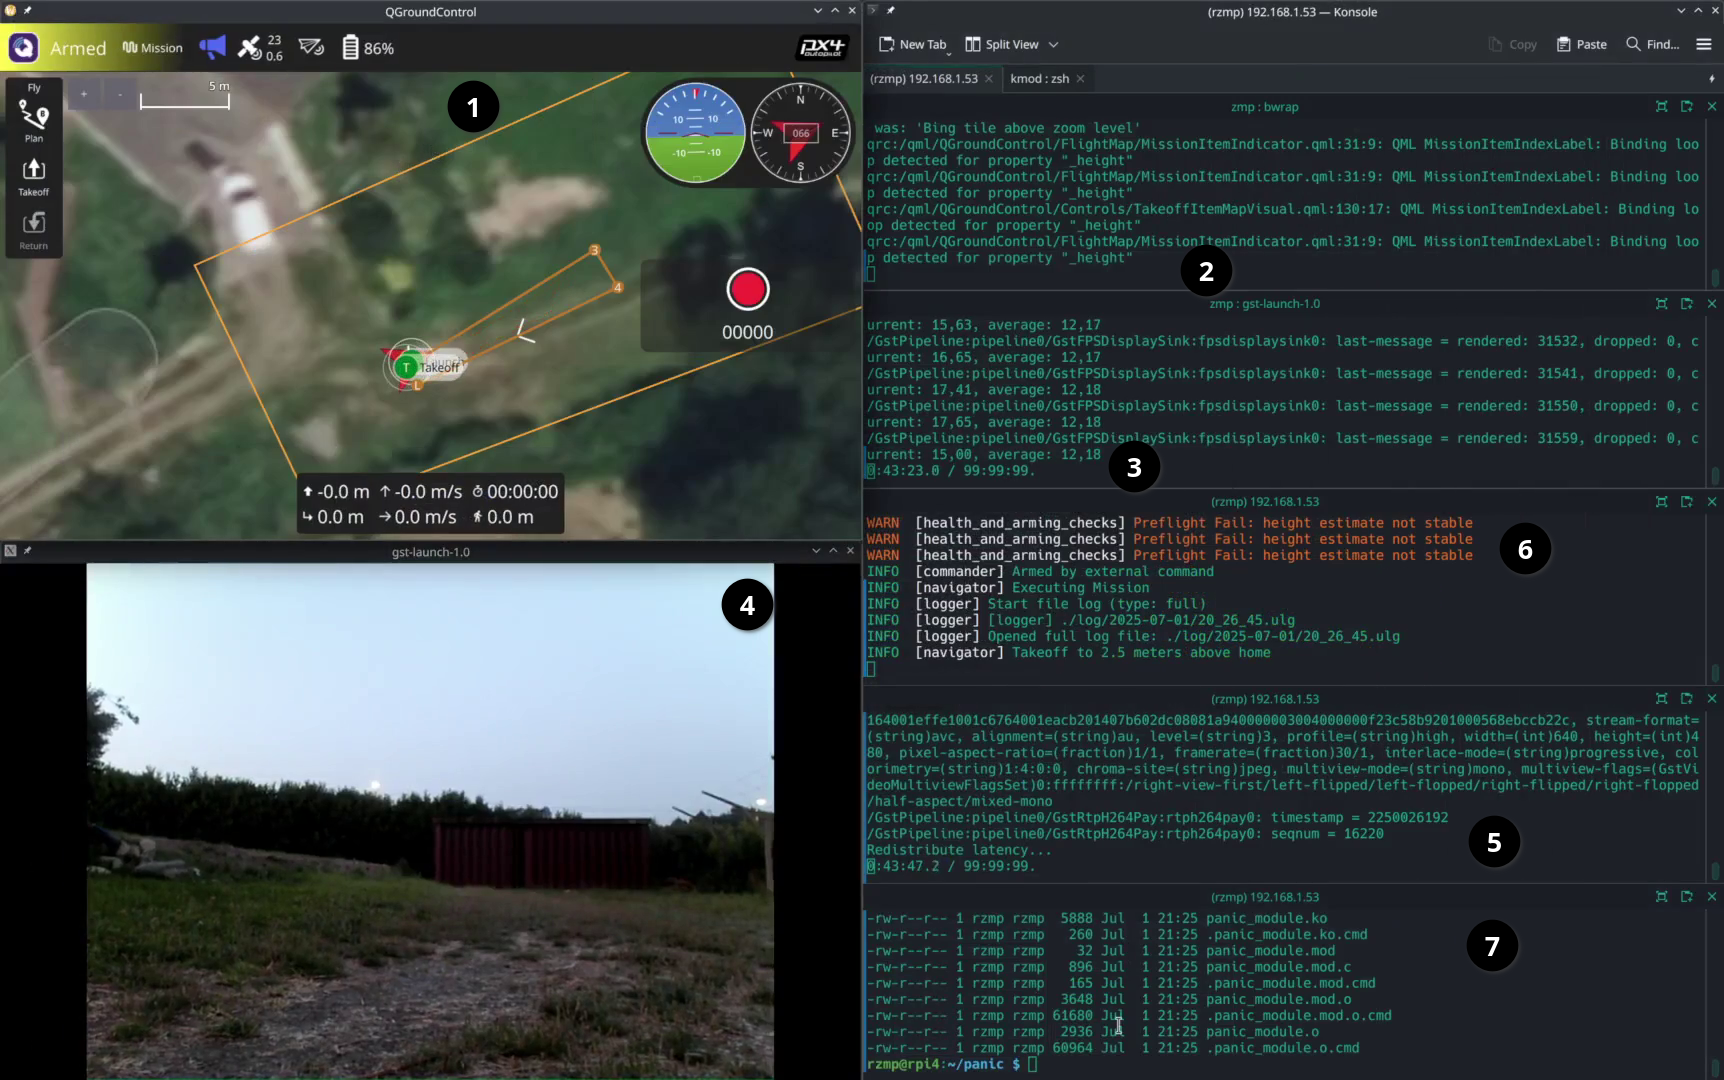
\includegraphics[width=1.0\textwidth]{./img/png/uspfs-crash-fpv-takeoff-annot} 
    \caption{UAV's view: takeoff}%
    \label{fig:mission-exec-uspfs-takeoff-1}
  \end{subfigure}
%  
  % Row 2: Two half-width images
  \begin{subfigure}[t]{0.49\textwidth}
    \centering
    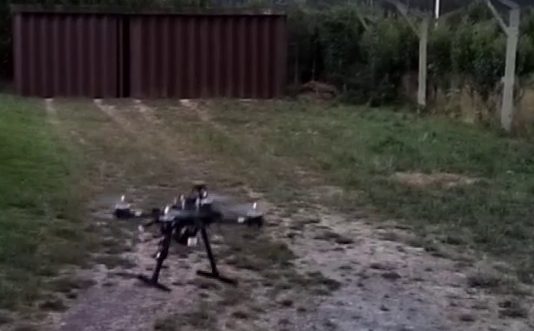
\includegraphics[width=0.98\linewidth]{./img/png/uspfs-crash-myView-takeoff-crop} % Use \linewidth inside subfigure
    \caption{Operator's view: takeoff}%
    \label{fig:mission-exec-uspfs-takeoff-2}
  \end{subfigure}
%  
  % Row 2: Two half-width images
  \begin{subfigure}[t]{0.49\textwidth}
    \centering
    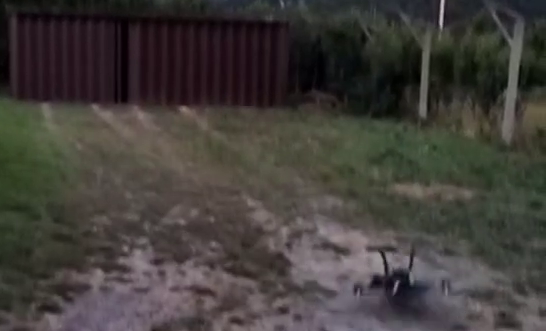
\includegraphics[width=\linewidth]{./img/png/uspfs-crash-myView-final-crop} % Use \linewidth inside subfigure
    \caption{Operator's view: UAV's crash}%
    \label{fig:mission-exec-uspfs-final}
  \end{subfigure}
%  
  \caption{Mission execution: functional test (USPFS)}
  \label{fig:mission-exec-uspfs}
\end{figure}


% \begin{figure}[!hbt]
%   \centering
%   % Row 1: Full width
%   \begin{subfigure}[t]{\textwidth}
%     \centering
%     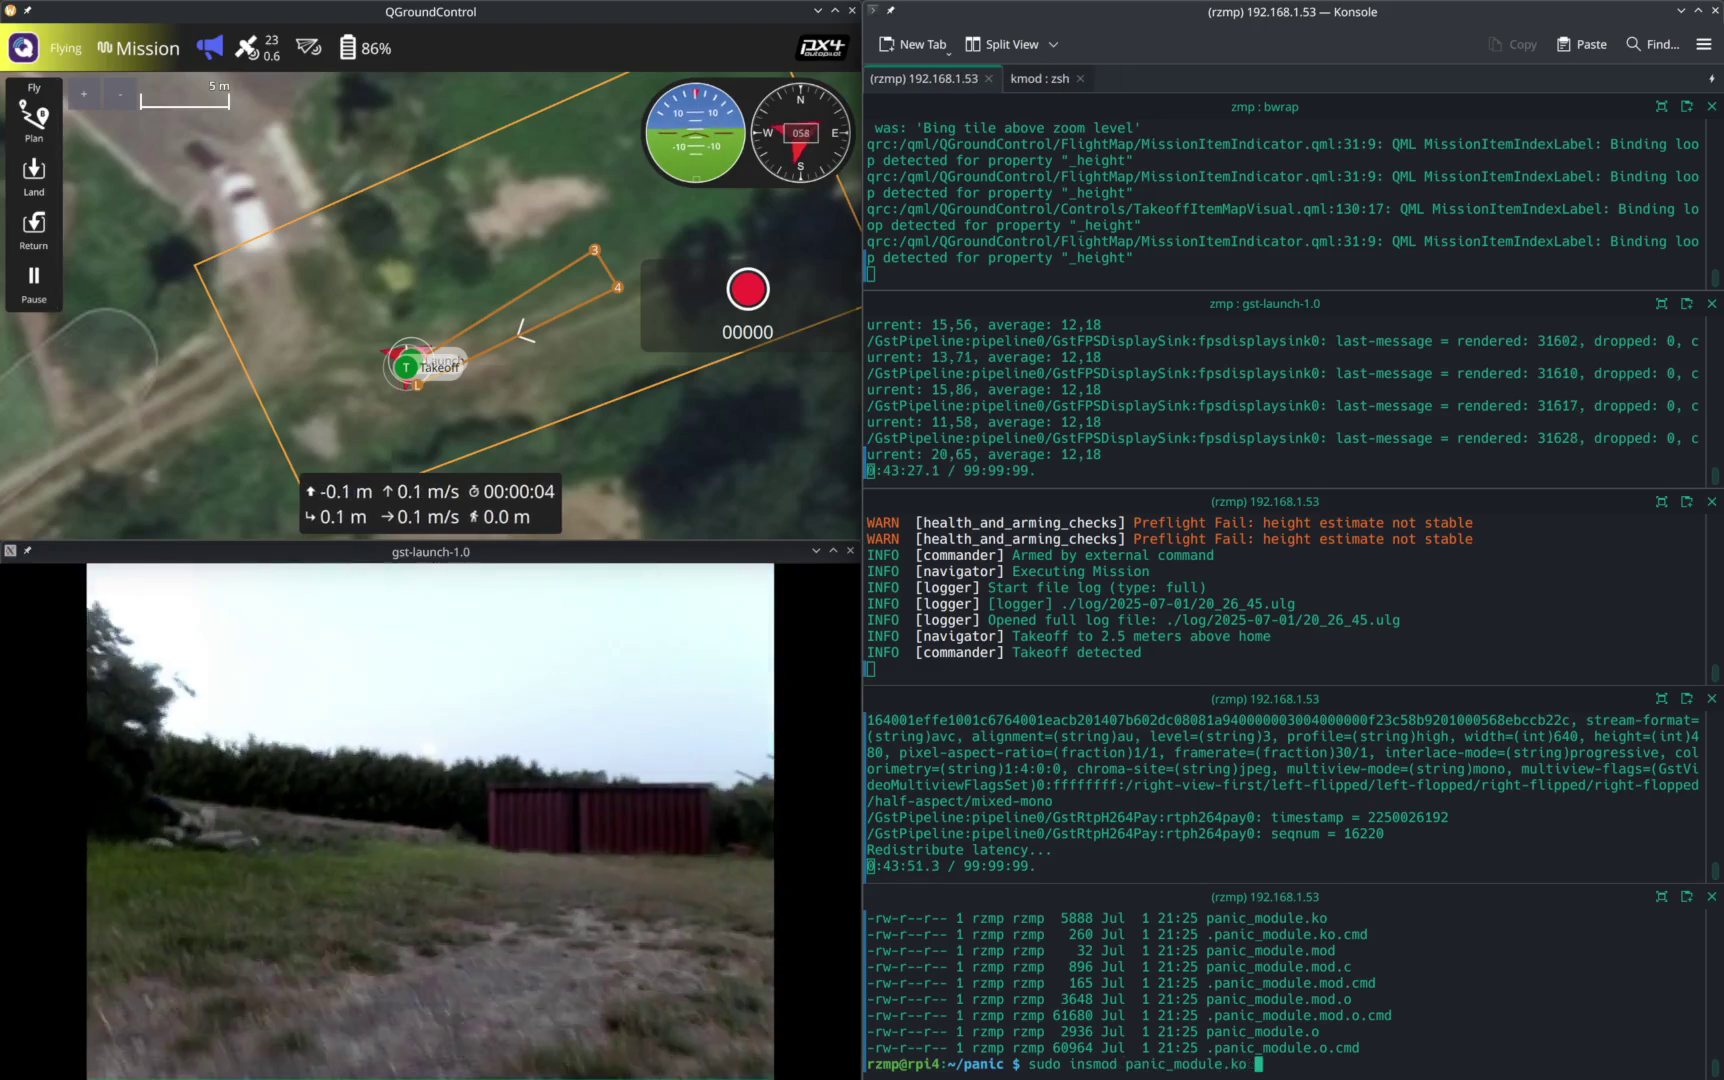
\includegraphics[width=1.0\textwidth]{./img/png/uspfs-crash-fpv-insmod} 
%     \caption{UAV's view}%
%     \label{fig:mission-exec-uspfs-insmod-1}
%   \end{subfigure}
% %  
%   % Row 2: Two half-width images
%   \begin{subfigure}[t]{0.49\textwidth}
%     \centering
%     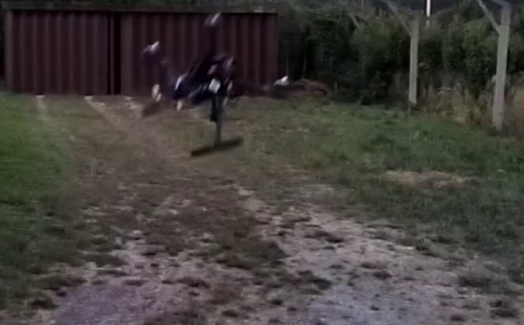
\includegraphics[width=\linewidth]{./img/png/uspfs-crash-myView-insmod-crop} % Use \linewidth inside subfigure
%     \caption{Operator's view}%
%     \label{fig:mission-exec-uspfs-insmod-2}
%   \end{subfigure}
% %  
%   \caption{Mission execution: Functional test (USPFS) -- executing a malicious kernel module}
%   \label{fig:mission-exec-uspfs-insmod}
% \end{figure}

% \begin{figure}[!hbt]
%   \centering
%   % Row 1: Full width
%   \begin{subfigure}[t]{\textwidth}
%     \centering
%     \includegraphics[width=1.0\textwidth]{./img/png/uspfs-crash-fpv-final} 
%     \caption{UAV's view}%
%     \label{fig:mission-exec-uspfs-final-1}
%   \end{subfigure}
% %  
%   % Row 2: Two half-width images
%   \begin{subfigure}[t]{0.49\textwidth}
%     \centering
%     \includegraphics[width=\linewidth]{./img/png/uspfs-crash-myView-final-crop} % Use \linewidth inside subfigure
%     \caption{Operator's view}%
%     \label{fig:mission-exec-uspfs-final-2}
%   \end{subfigure}
% %  
%   \caption{Mission execution: Functional test (USPFS) -- UAV's crash}
%   \label{fig:mission-exec-uspfs-final}
% \end{figure}

% \section{Summary}
% \label{sec:summary-eval}
% This chapter presented testing and evaluation of the proposed solution. Functional testing analyzed unsupervised (\gls{uspfs}) and supervised (\gls{sspfs}) system behavior under compromise scenarios. Multiple attack approaches were examined across privileged and unprivileged execution modes. Privileged compromise enables system hijacking through malicious kernel modules inducing system halting (\lstinline{panic}), memory corruption, resource exhaustion, or termination of the \lstinline{init} process. Unprivileged attacks are constrained to user-space exploits, substantially reducing the attack surface, typically manifesting as resource contention that significantly degrades system performance. \gls{uspfs} compromise causes simultaneous failure of critical \gls{fmu} and non-critical video surveillance stacks, resulting in total system failure. Conversely, \gls{sspfs} containment prevents non-critical stack failures from propagating to the critical domain, maintaining \gls{uav} operation despite video streaming interruption. These results demonstrate Bao hypervisor's capability to consolidate mixed-criticality software stacks on a single platform while ensuring domain isolation.

% Benchmarking compared \gls{uspfs} baseline performance against \gls{sspfs} degradation introduced by the Bao hypervisor using the MiBench \glsxtrfull{aics} suite. Analysis included guest interference effects and Raspberry Pi firmware mailbox driver modifications. Results indicate negligible performance degradation attributable to either Bao or mailbox patches. However, significant performance degradation occurs under interference conditions, particularly for shorter benchmarks, though this effect diminishes over execution duration. Cache partitioning via page coloring consistently reduces VM1 performance degradation, demonstrating utility for interference mitigation.

% Guest benchmarking in single- and dual-\gls{vm} configurations evaluated PX4 task scheduling overhead and camera frame rates. Bao introduces minimal scheduling overhead (≤2\% worst-case) in the critical system and statistically insignificant frame rate impact. Comparative analysis reveals that beyond isolation benefits, the supervised \gls{sspfs} solution offers potential performance advantages through static resource partitioning.

% Real-flight evaluation employed automated missions to compare position tracking and resource utilization. Supervision introduction shows no position tracking degradation, with modest \gls{cpu} overhead (6\% average). Significant \gls{ram} expansion (99 KB) is attributed to firmware mailbox supervision requiring Bao's mailbox manager transaction handling. Verification would require alternative \gls{vm} device-sharing mechanisms, currently unavailable. This \gls{ram} increase remains operationally negligible given the \gls{fmu} \gls{vm}'s 144 MB allocation. Repeated functional tests confirmed critical stack resilience during non-critical failures. Consequently, \gls{sspfs} emerges as the optimal solution for consolidating mixed-criticality \gls{fmu} and video surveillance stacks, providing robust isolation guarantees with minimal performance overhead.

%%% Local Variables:
%%% mode: latex
%%% TeX-master: "../template"
%%% reftex-default-bibliography: ("../Bibliography/mieeic.bib")
%%% ispell-local-dictionary: "american"
%%% End:
